%%% The main file. It contains definitions of basic parameters and includes all other parts.

% Meta-data of your thesis (please edit)
\input metadata.tex

% Generate metadata in XMP format for use by the pdfx package
\input xmp.tex

%% Settings for single-side (simplex) printing
% Margins: left 40mm, right 25mm, top and bottom 25mm
% (but beware, LaTeX adds 1in implicitly)
\documentclass[12pt,a4paper]{report}



\setlength\textwidth{145mm}
\setlength\textheight{247mm}
\setlength\oddsidemargin{15mm}
\setlength\evensidemargin{15mm}
\setlength\topmargin{0mm}
\setlength\headsep{0mm}
\setlength\headheight{0mm}
% \openright makes the following text appear on a right-hand page
\let\openright=\clearpage

%% Settings for two-sided (duplex) printing
% \documentclass[12pt,a4paper,twoside,openright]{report}
% \setlength\textwidth{145mm}
% \setlength\textheight{247mm}
% \setlength\oddsidemargin{14.2mm}
% \setlength\evensidemargin{0mm}
% \setlength\topmargin{0mm}
% \setlength\headsep{0mm}
% \setlength\headheight{0mm}
% \let\openright=\cleardoublepage

%% If the thesis has no printed version, symmetric margins look better
% \documentclass[12pt,a4paper]{report}
% \setlength\textwidth{145mm}
% \setlength\textheight{247mm}
% \setlength\oddsidemargin{10mm}
% \setlength\evensidemargin{10mm}
% \setlength\topmargin{0mm}
% \setlength\headsep{0mm}
% \setlength\headheight{0mm}
% \let\openright=\clearpage

%% Generate PDF/A-2u
\usepackage[a-2u]{pdfx}

%% Prefer Latin Modern fonts
\usepackage{lmodern}
% If we are not using LuaTeX, we need to set up character encoding:
\usepackage{iftex}
\ifpdftex
\usepackage[utf8]{inputenc}
\usepackage[T1]{fontenc}
\usepackage{textcomp}
\fi

%% Further useful packages (included in most LaTeX distributions)
\usepackage{amsmath}        % extensions for typesetting of math
\usepackage{amsfonts}       % math fonts
\usepackage{amsthm}         % theorems, definitions, etc.
\usepackage{bm}             % boldface symbols (\bm)
\usepackage{booktabs}       % improved horizontal lines in tables
\usepackage{caption}        % custom captions of floating objects

\usepackage{tabularx}
\usepackage{array}
\usepackage{subcaption}
%\usepackage{cleveref}
\usepackage[sort,noabbrev]{cleveref}


\usepackage{dcolumn}        % improved alignment of table columns
\usepackage{floatrow}       % custom float environments
\usepackage{graphicx}       % embedding of pictures
\usepackage{indentfirst}    % indent the first paragraph of a chapter
\usepackage[nopatch=item]{microtype}   % micro-typographic refinement
\usepackage{paralist}       % improved enumerate and itemize
\usepackage[nottoc]{tocbibind} % makes sure that bibliography and the lists
			    % of figures/tables are included in the table
			    % of contents
\usepackage{xcolor}         % typesetting in color

% The hyperref package for clickable links in PDF and also for storing
% metadata to PDF (including the table of contents).
% Most settings are pre-set by the pdfx package.
\hypersetup{unicode}
\hypersetup{breaklinks=true}

% Packages for computer science theses
\usepackage{algpseudocode}  % part of algorithmicx package
\usepackage{algorithm}
\usepackage{fancyvrb}       % improved verbatim environment
\usepackage{listings}       % pretty-printer of source code

\definecolor{darkyellow}{rgb}{1.0, 0.8, 0.0} % Define a darker yellow color
\definecolor{green}{rgb}{0.0, 0.7, 0.0}

% You might want to use cleveref for references
% \usepackage{cleveref}

% Set up formatting of bibliography (references to literature)
% Details can be adjusted in macros.tex.
%
% BEWARE: Different fields of research and different university departments
% have their own customs regarding bibliography. Consult the bibliography
% format with your supervisor.
%
% The basic format according to the ISO 690 standard with numbered references
\usepackage[natbib,style=iso-numeric,sorting=none]{biblatex}
% ISO 690 with alphanumeric references (abbreviations of authors' names)
%\usepackage[natbib,style=iso-alphabetic]{biblatex}
% ISO 690 with references Author (year)
%\usepackage[natbib,style=iso-authoryear]{biblatex}
%
% Some fields of research prefer a simple format with numbered references
% (sorting=none tells that bibliography should be listed in citation order)
%\usepackage[natbib,style=numeric,sorting=none]{biblatex}
% Numbered references, but [1,2,3,4,5] is compressed to [1-5]
%\usepackage[natbib,style=numeric-comp,sorting=none]{biblatex}
% A simple format with alphanumeric references:
%\usepackage[natbib,style=alphabetic]{biblatex}

\crefname{enumi}{}{}
\creflabelformat{enumi}{\textbf{R#2#1#3}}


% Load the file with bibliography entries
\addbibresource{bibliography.bib}

% Our definitions of macros (see description inside)
\input macros.tex

%%% Title page and various mandatory informational pages
\begin{document}
%%% Title page of the thesis and other mandatory pages

%%% Inscriptions at the opening page of the hard cover

% We usually do not typeset the hard cover, but if you want to do it, change \iffalse to \iftrue
\iffalse

\pagestyle{empty}
\hypersetup{pageanchor=false}
\begin{center}

\large
Charles University

\medskip

Faculty of Mathematics and Physics

\vfill

{\huge\bf\ThesisTypeTitle}

\vfill

{\huge\bf\ThesisTitle\par}

\vfill
\vfill

\hbox to \hsize{\YearSubmitted\hfil \ThesisAuthor}

\end{center}

\newpage\openright
\setcounter{page}{1}

\fi

%%% Title page of the thesis

\pagestyle{empty}
\hypersetup{pageanchor=false}
\begin{center}

\centerline{\mbox{
\includegraphics[width=166mm]{img/logo-en.pdf}}}

\vspace{-8mm}
\vfill

{\bf\Large\ThesisTypeTitle}

\vfill

{\LARGE\ThesisAuthor}

\vspace{15mm}

{\LARGE\bfseries\ThesisTitle\par}

\vfill

\Department

\vfill

{
\centerline{\vbox{\halign{\hbox to 0.45\hsize{\hfil #}&\hskip 0.5em\parbox[t]{0.45\hsize}{\raggedright #}\cr
Supervisor of the \ThesisTypeName{} thesis:&\Supervisor \cr
\ifx\ThesisType\TypeRig\else
\noalign{\vspace{2mm}}
Study programme:&\StudyProgramme \cr
\fi
}}}}

\vfill

Prague \YearSubmitted

\end{center}

\newpage

%%% A page with a solemn declaration to the thesis

\openright
\hypersetup{pageanchor=true}
\vglue 0pt plus 1fill

\noindent
I declare that I carried out this \ThesisTypeName{} thesis on my own, and only with the cited
sources, literature and other professional sources.
I understand that my work relates to the rights and obligations under the Act No.~121/2000 Sb.,
the Copyright Act, as amended, in particular the fact that the Charles
University has the right to conclude a license agreement on the use of this
work as a school work pursuant to Section 60 subsection 1 of the Copyright~Act.

\vspace{10mm}

\hbox{\hbox to 0.5\hsize{%
In \hbox to 6em{\dotfill} date \hbox to 6em{\dotfill}
\hss}\hbox to 0.5\hsize{\dotfill\quad}}
\smallskip
\hbox{\hbox to 0.5\hsize{}\hbox to 0.5\hsize{\hfil Author's signature\hfil}}

\vspace{20mm}
\newpage

%%% Dedication

\openright

\noindent
\Dedication

\newpage

%%% Mandatory information page of the thesis

\openright
{\InfoPageFont

\vtop to 0.5\vsize{
\setlength\parindent{0mm}
\setlength\parskip{5mm}

Title:
\ThesisTitle

Author:
\ThesisAuthor

\DeptType:
\Department

Supervisor:
\Supervisor, \SupervisorsDepartment

Abstract:
\Abstract

Keywords:
{\def\sep{\unskip, }\ThesisKeywords}

\vfil
}

% In Czech study programmes, it is mandatory to include Czech meta-data:

\ifx\StudyLanguage\LangCS

\vtop to 0.49\vsize{
\setlength\parindent{0mm}
\setlength\parskip{5mm}

Název práce:
\ThesisTitleCS

Autor:
\ThesisAuthor

\DeptTypeCS:
\DepartmentCS

Vedoucí bakalářské práce:
\Supervisor, \SupervisorsDepartmentCS

Abstrakt:
\AbstractCS

Klíčová slova:
{\def\sep{\unskip, }\ThesisKeywordsCS}

\vfil
}

\fi

}

\newpage

%%% Further pages will be numbered
\pagestyle{plain}


%%% A page with automatically generated table of contents of the thesis

\tableofcontents

%%% Each chapter is kept in a separate file
\chapter*{Introduction}
\addcontentsline{toc}{chapter}{Introduction}


\chapter{Problem analysis}

This chapter provides details on the problem the application is trying to solve and describes user requirements specifying what functionality the application should provide to its users. It also includes an overview of existing solutions for the connection search problem. Finally, it describes the available data necessary to provide the functionality and its structure.

\section{Problem description}

We will first introduce the problem's domain and explain all the necessary terms we will be using later. Then we will describe the core of the problem our application is trying to solve.

\subsection{Domain introduction}

\begin{figure}[h!]
    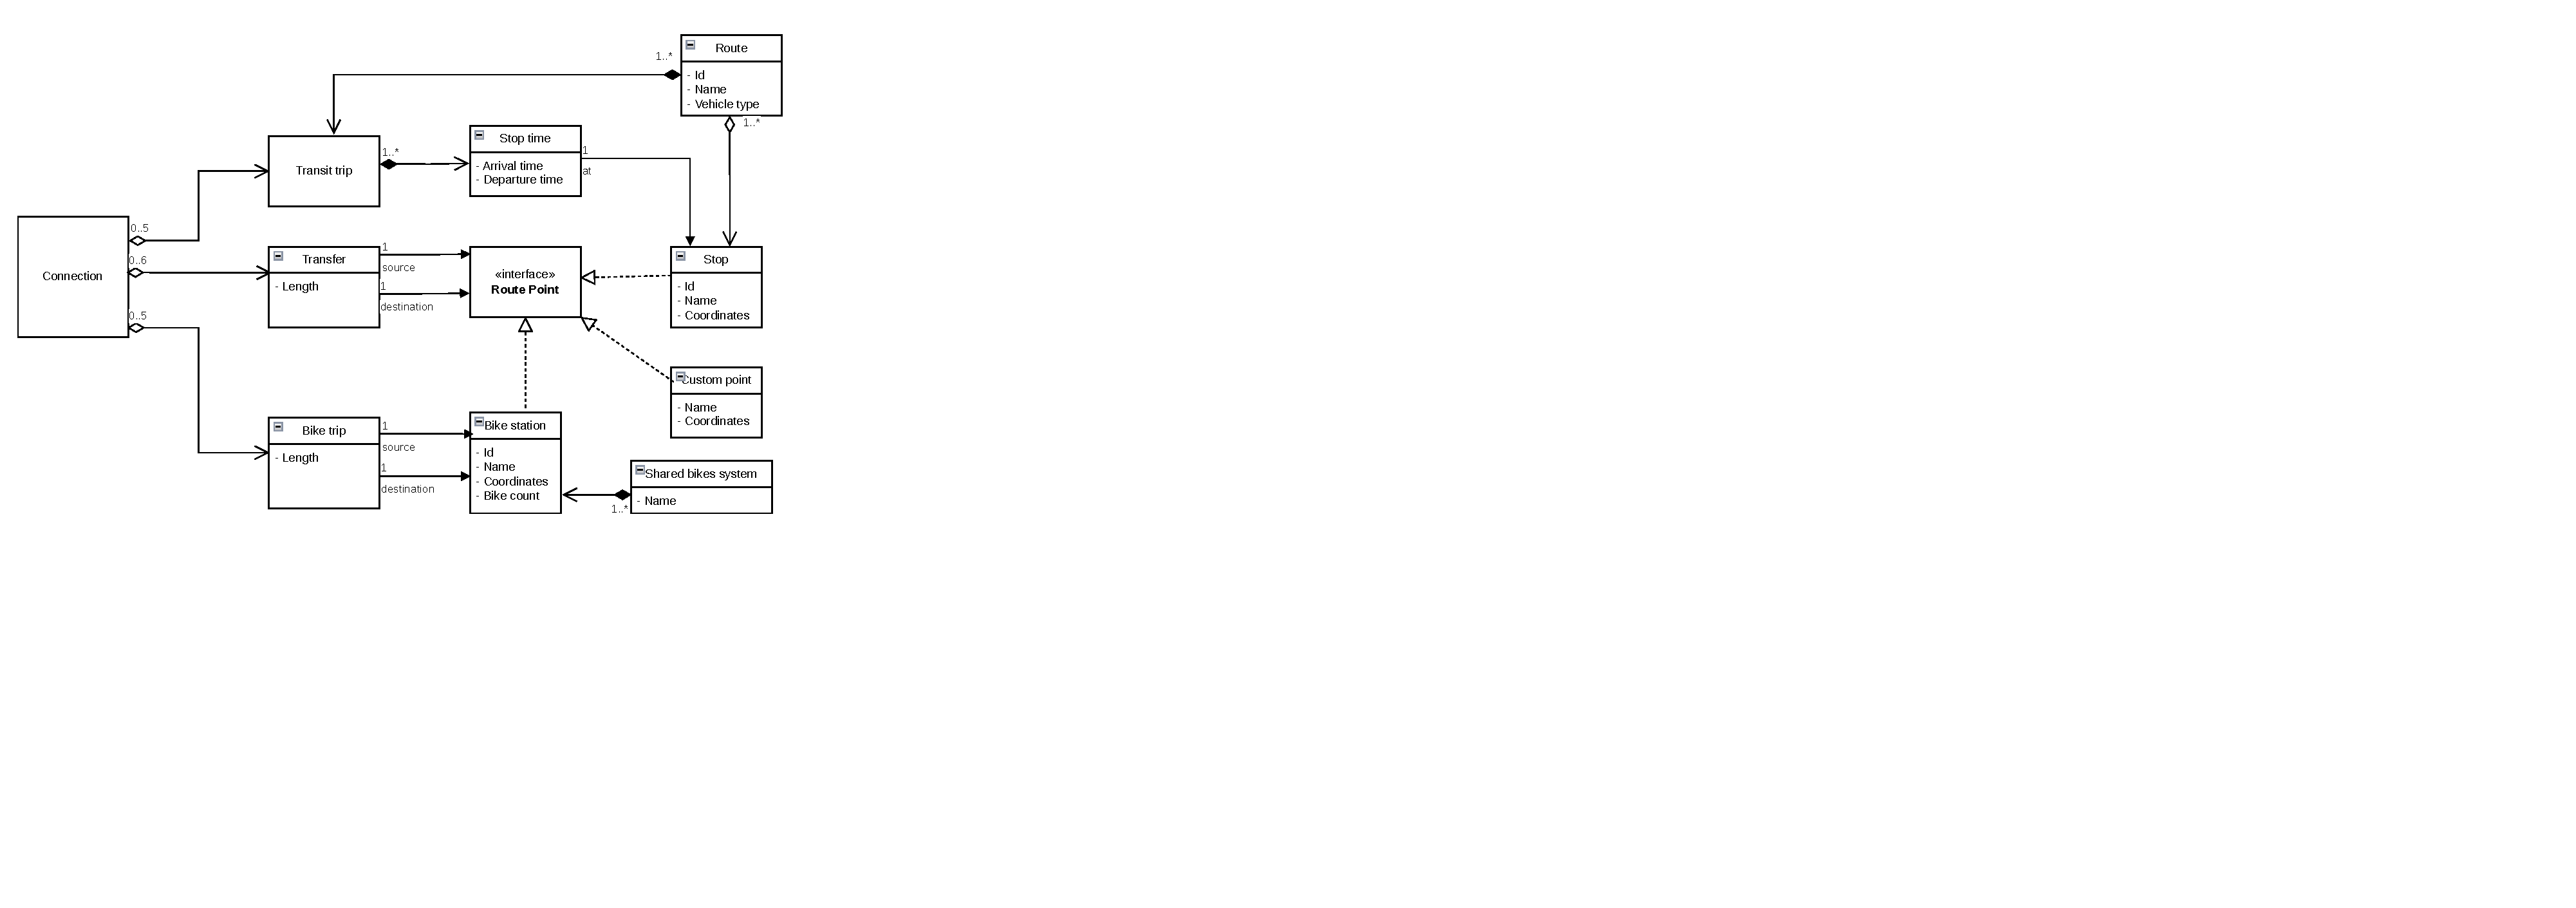
\includegraphics[width=\textwidth]{img/domain_model.pdf}
    \caption{The domain model}
    \label{fig:domain_model}
\end{figure}

The result that we want to produce and show to the user is a \texttt{Connection}. A \texttt{Connection} consists of public transit \texttt{Trips}, \texttt{Transfers} and \texttt{Bike trips}. 

Every \texttt{Trip} serves one \texttt{Route}. A \texttt{Route} consists of a sequence of \texttt{Stops} and typically corresponds to what is usually known as a line. Every \texttt{Route} has a name and a vehicle type describing what vehicle the \texttt{Route} is being served by (i.e. Bus/Tram/Metro/...). However, it is important to note that the relationship between a \texttt{Route} within the context of our application and a real-world public transit line is not 1:1. Typically, one line will have multiple different variations (shorter variations, variations with vehicles pulling in and out of the depots, variations where not all stops are served, ...). All of these variations will share the same line name, however, each of them is a separate \texttt{Route} with its separate sequence of \texttt{Stops}.

A \texttt{Trip} corresponds to an actual trip of a public transit vehicle and serves a single \texttt{Route}. It consists of a sequence of \texttt{Stop Times}. A \texttt{Stop Time} specifies both the arrival and departure times of the \texttt{Trip} at the corresponding \texttt{Stop} of the \texttt{Trip}'s \texttt{Route}.

A \texttt{Transfer} represents travel on foot. It consists of two points - the source and the destination \texttt{Route Points}. A \texttt{Route Point} can be either a \texttt{Stop}, a \texttt{Bike Station} or a \texttt{Custom point}.

A \texttt{Stop} represents a single point within the public transit network where it is possible to board or disembark public transit \texttt{Trips}. It is important to mention that a \texttt{Stop} within the context of our application does not directly correspond to what most people imagine under the term. Typically, a "stop" is described by its name, i.e. all boarding points sharing the same name are considered a single "stop". In our context, every single one of these boarding points is its own separate \texttt{Stop}. Within Prague's public transit network, this typically means that each \texttt{Stop} corresponds to a separate stop sign. The set of \texttt{Stops} sharing the same name is called a \texttt{Node}.

A \texttt{Custom point} is an arbitrary point within the connection, specified by its coordinates. Typically, it will be used to provide the user with the opportunity to set the source or target of his search to a specific coordinate point, instead of having to always select a specific \texttt{Stop} or \texttt{Node}.

Finally, a \texttt{Bike Trip} represents travel on a shared bicycle. It consists of a source and destination \texttt{Bike Station}. A \texttt{Bike Station} is a single point within a particular \texttt{Bikesharing system} at which it is possible to borrow and return bicycles. Every \texttt{Bikesharing System} has its own set of \texttt{Bike Stations}, each of which has a name (typically describing its location) and coordinate location and has a certain number of currently available bicycles in it. A \texttt{Bike Trip} cannot be performed between \texttt{Bike Stations} that belong to different \texttt{Bikesharing Systems}.

To collectively describe the three different parts of a \texttt{Connection} (\texttt{Trips}, \texttt{Transfers} and \texttt{Bike Trips}), we will use the term \texttt{Segments}.


\subsection{Core problem definition}

The core problem the application is trying to solve is the connection search problem. The user needs to be able to use the app to search for efficient connections between two points within Prague's public transit network that they specify. Furthermore, to account for both use cases where the user wants to depart after a certain time and where they want to arrive before a certain time, the application will need to be able to handle both of these options. The application needs to be able to find and show this resulting connection (or multiple alternative connections) to the user.

As stated above, each connection will consist of trips, transfers and bike trips. Between any 2 consecutive trips within a connection, there may be any number of transfers or bike trips. This means that if the connection contains two or more public transit trips, for any 2 consecutive trips within the connection, the sum of durations of the transfers and bike trips between them needs to be less than or equal to the length of the time frame between the first trip's disembark time and the second trip's boarding time.

Furthermore, it is not allowed for two transfers to follow immediately after one another. The same is true for bike trips. This is to prevent the chaining of transfers or bike trips, which would render it useless to set a maximum time or distance for them. It is theoretically possible for 2 trips to follow directly after one another as the first one may arrive at the same exact stop as the second one departs, but for simplicity's sake, we will require a 0 meter long transfer to be inserted in between them in such situations. This means that within the list of trips, transfers and bike trips that a connection consists of, two segments of the same type may never occur directly consecutively.

Apart from the inclusion of bikesharing, this is the core functionality that any connection planning application must provide. The main goal of our application is to expand this functionality to provide more useful personalization options. These additional problems, features and solutions will be described in following chapters.

\section{Existing solutions}

As stated above, the goal of this application is to provide people living and working in Prague with a practical way to search for connections within Prague's extensive public transit network. However, there already are many existing solutions serving the purpose of searching for public transit connections, so why is it necessary to develop another one? To answer this question, we will go over the existing solutions and describe their advantages and shortcomings. From this information, we will derive the requirements for our new, improved way to approach the problem.

The core functionality we explained in the previous chapter is identical for all existing solutions. For this reason, in this chapter we will only describe the functionality each of the solutions provides on top of this.

\subsection{Global solutions}

First of all, there are many solutions for public transit connection searching that promise to work worldwide and could thus also be used within Prague.

\subsubsection{Maps Google}
In addition to car and pedestrian routing, Google's Maps also provide routing between 2 points using public transportation. On top of the basics, they also include the option to prioritize certain transport modes and basic filtering options based on the user's preferences ("Best route", "Fewer transfers", "Less walking", "Wheelchair accessible"). However, the application also has many shortcomings for a regular public transit user. For instance, there is no way to adjust one's walking pace, search for the absolute fastest connections or to set the maximum distance of transfers and the app does not support bikesharing in its search. The app also does not properly support searching using stop names and uses local names and points of interest instead. Arguably the biggest drawback is the app's UI. While being practical for infrequent long-distance connections by providing an overview of general route options, it is very hard to compare the options and find the most suitable one, making this app impractical for short public transit connections within the city (\cref{fig:google_maps_1}). Furthermore, as there is no way to search for a connection without displaying the map, this application is also very data-intensive, which is not desired in a connection searching app.

\begin{figure}[h!]
    \begin{minipage}[b]{0.45\textwidth}
        \centering
        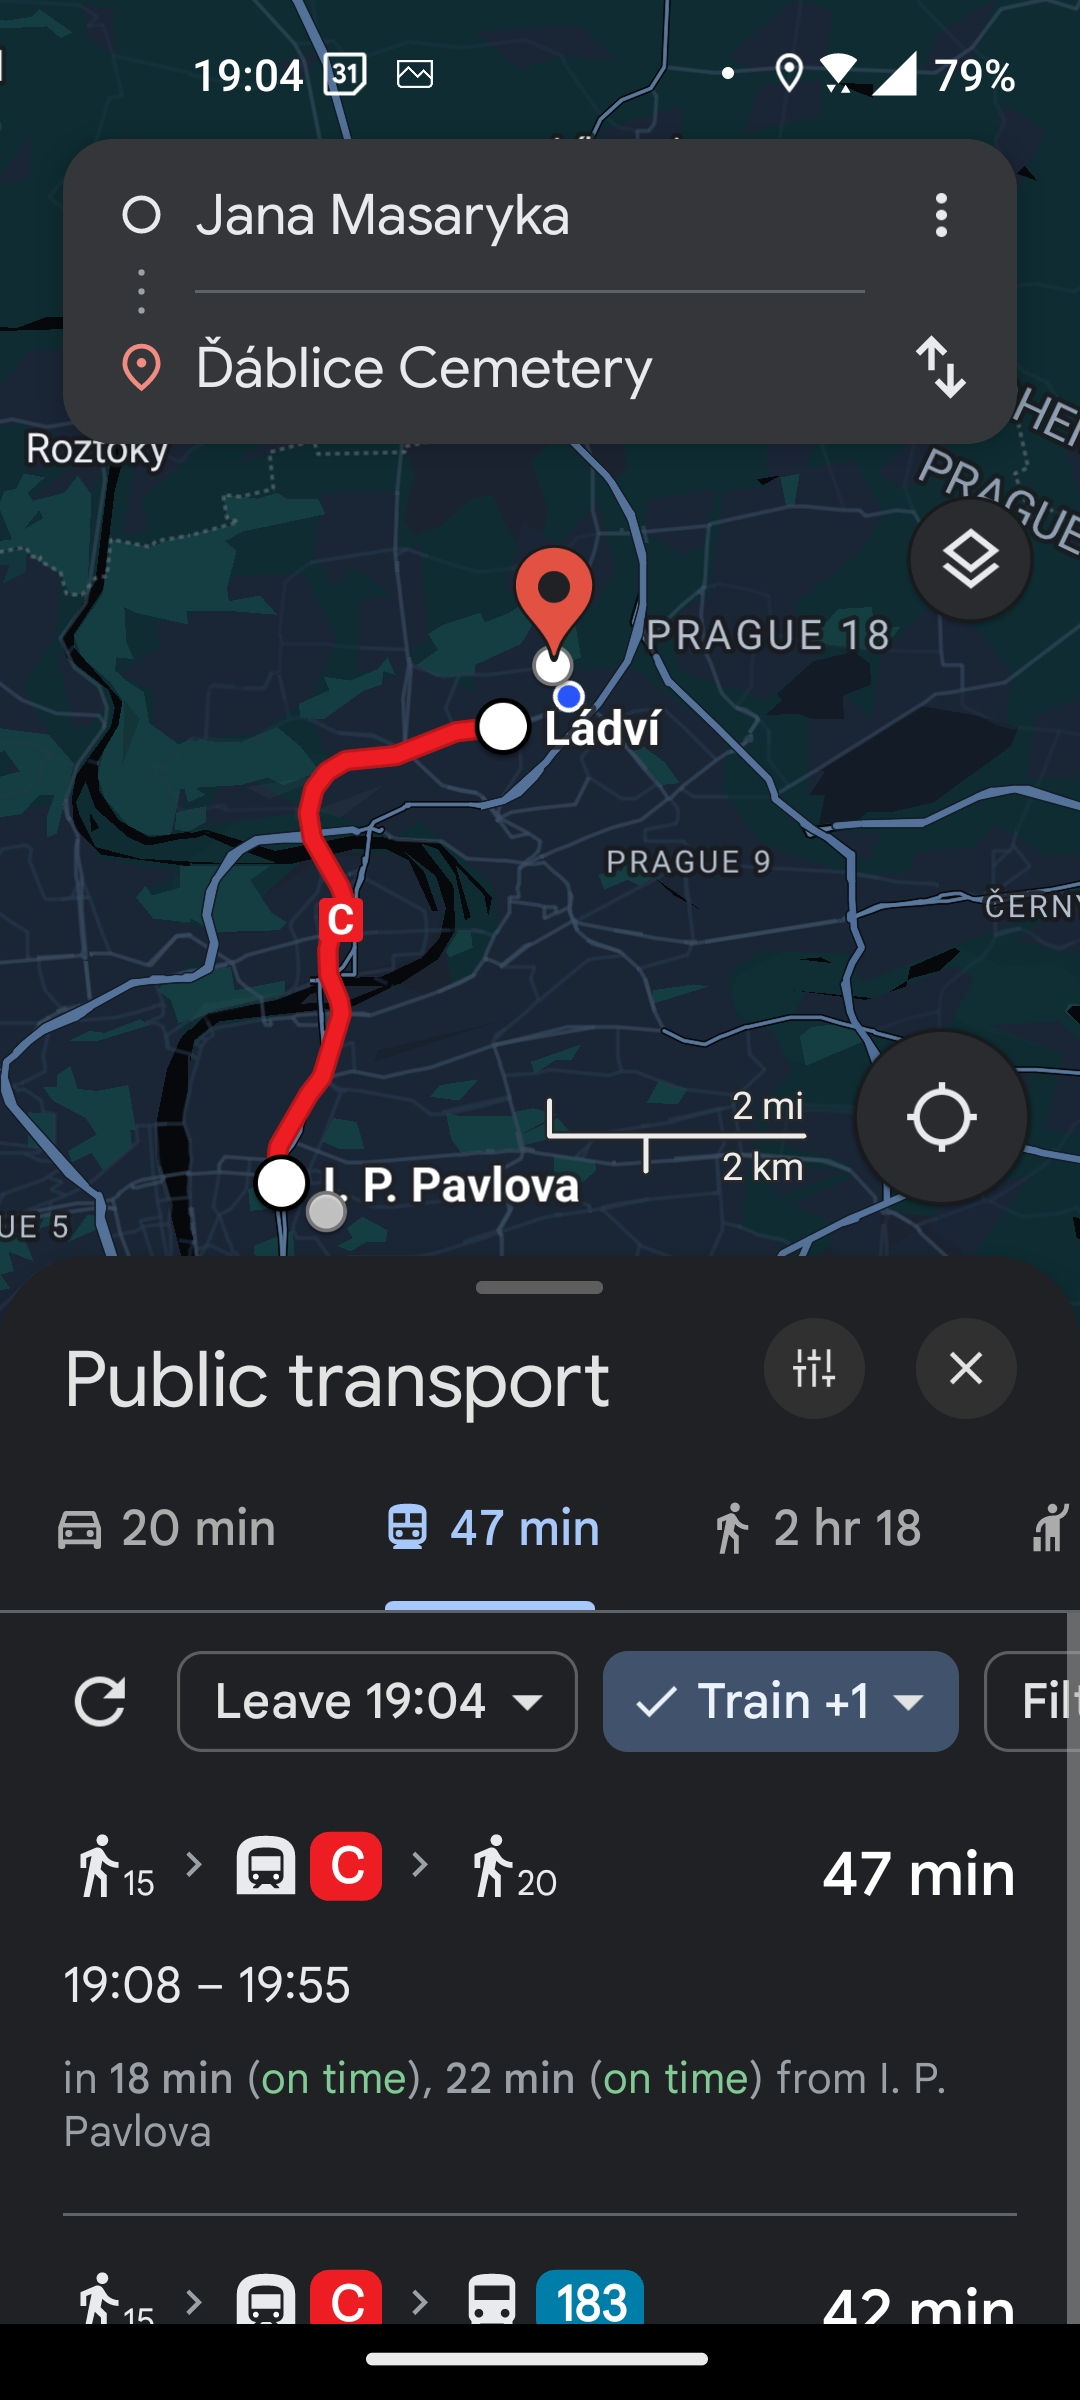
\includegraphics[width=\textwidth]{img/screenshots/google_maps_result_1.jpg}
    \end{minipage}
    \hfill
    \begin{minipage}[b]{0.45\textwidth}
        \centering
        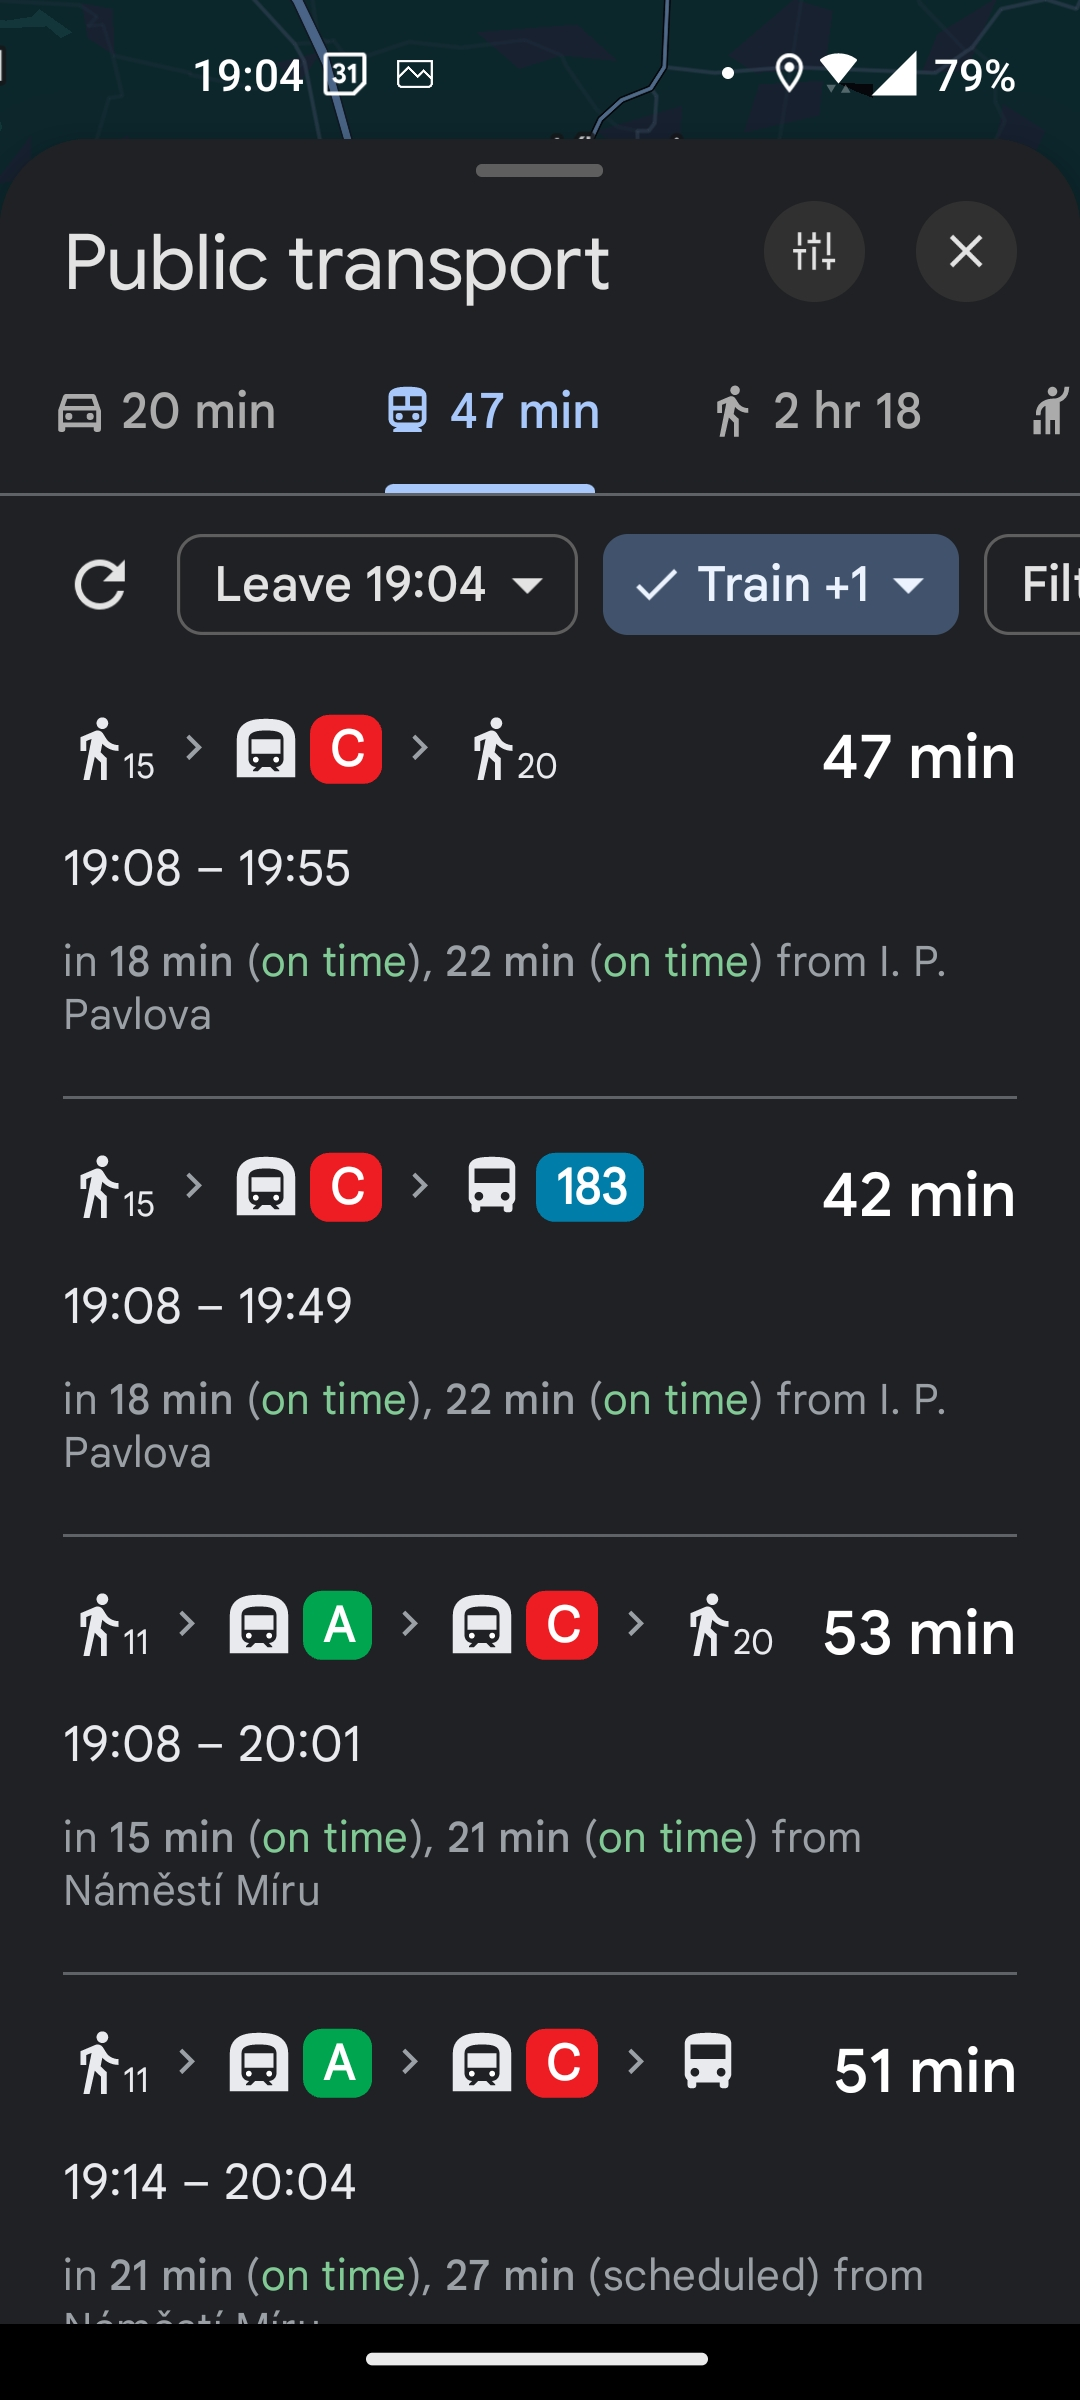
\includegraphics[width=\textwidth]{img/screenshots/google_maps_result_2.jpg}
    \end{minipage}
    \caption{Result of a connection search in Maps Google}
    \label{fig:google_maps_1}
\end{figure}

\subsubsection{Moovit}
Another option with global coverage is the Moovit app. Once again, there are some comfort preference setting options ("Best route", "Least walking", "Fewest transfers") and transit mode preference settings. This app also has an additional option for setting walking pace to slow, though there is no option for setting it to a specific value. The user can also set the maximum walk duration and search using stop names. However, the app also has many of the same issues as Google Maps, such as a distracting and confusing UI (\cref{fig:moovit}) and the lack of bikesharing support in Prague.



\begin{figure}[h!]
    \centering
    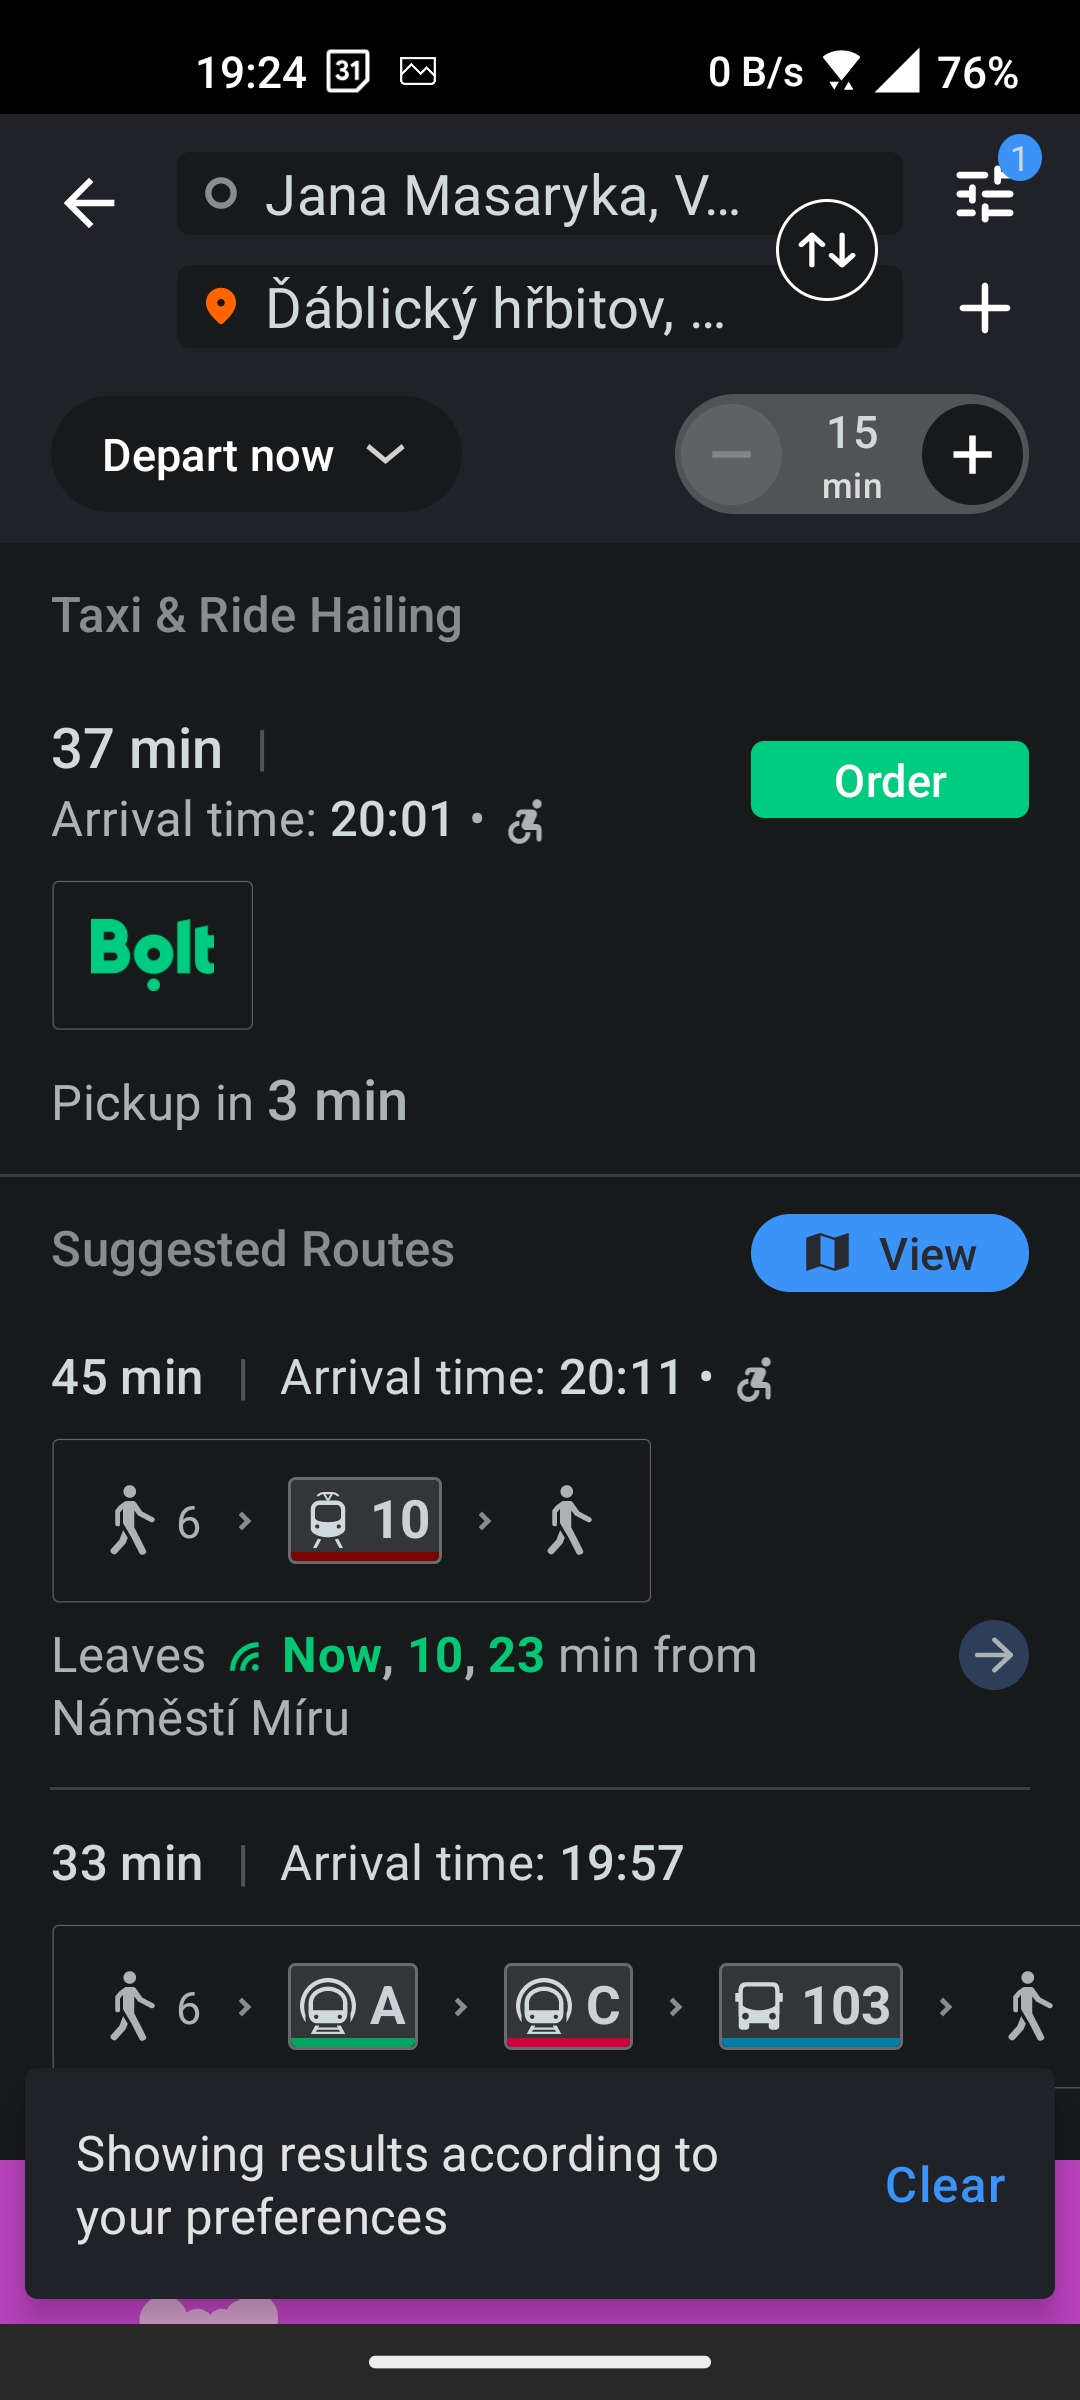
\includegraphics[width=0.45\textwidth]{img/screenshots/moovit_result.jpg}
    \caption{Result of a connection search in Moovit}
    \label{fig:moovit}
\end{figure}

\subsection{Country-wide solutions}

There also are some apps intended for the whole of Czech Republic, such as the following:

\subsubsection{IDOS}

IDOS is the most popular app for public transit connection searching in the Czech Republic. However, its search customization options are very limited. There are options for adding an intermediate stop, selecting transport modes and operators, only searching for direct connections, setting an absolute global transfer time and searching for wheelchair accessible connections. It lacks features such as comfort preference settings other than a direct connection search, setting maximum walking distance or walking pace or using bikesharing services. As opposed to many other apps, IDOS will also not consider connections starting from a different stop than the one entered by the user, even if it were a relatively short transfer and it would greatly reduce the arrival time. However, IDOS's UI is much more intuitive and practical for city-level public transit trips than those of the global apps, enabling the user to gain a better overview of their options through scrolling through all the available connections (\cref{fig:idos}).

\begin{figure}[h!]
    \centering
    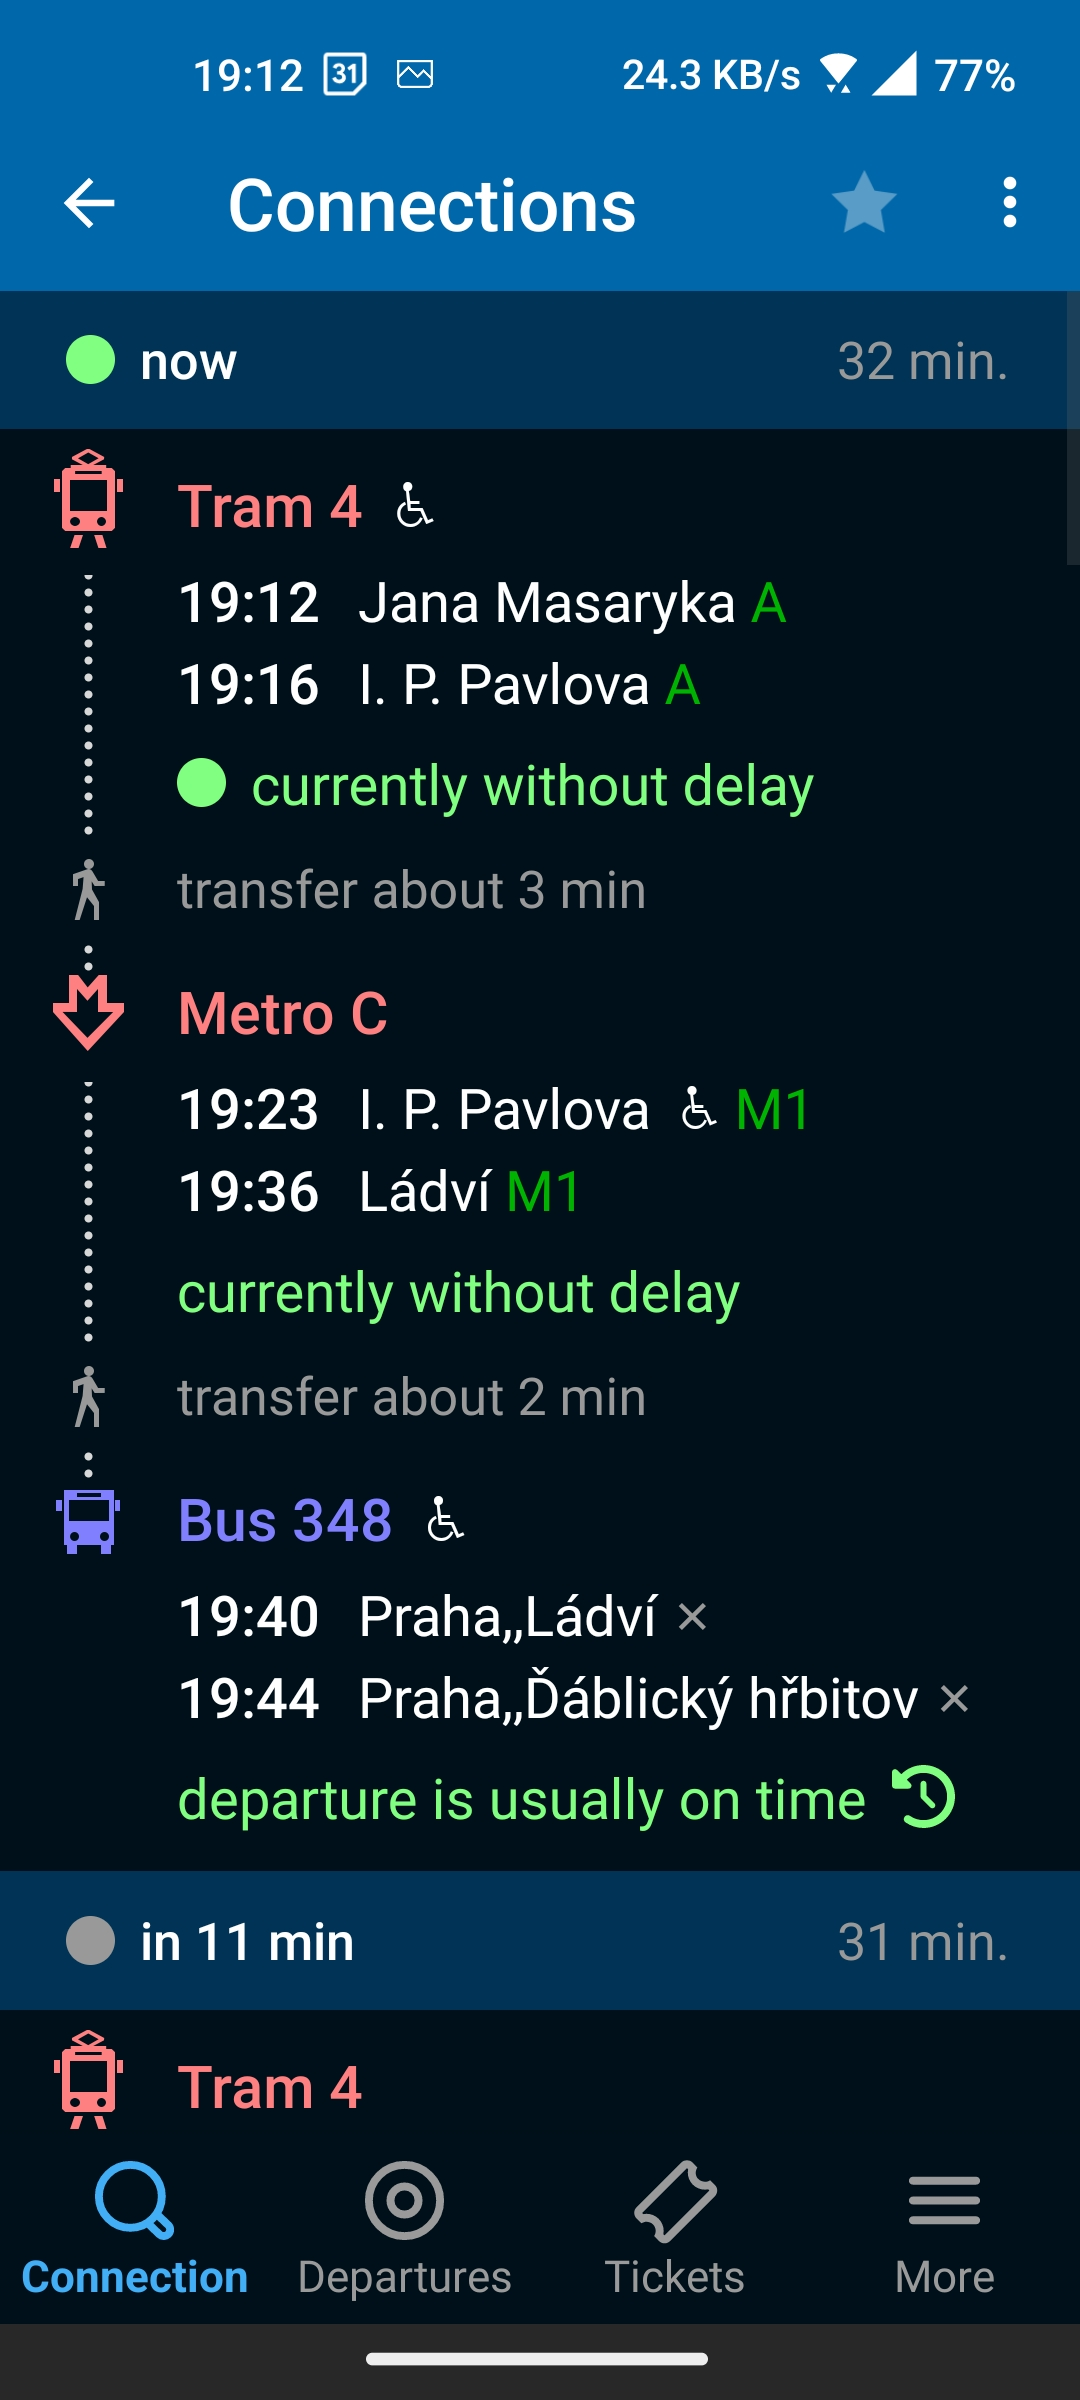
\includegraphics[width=0.45\textwidth]{img/screenshots/idos_result.jpg}
    \caption{Result of a connection search in IDOS}
    \label{fig:idos}
\end{figure}


\subsubsection{Pubtran}

Pubtran is another nation-wide option, developed by the Czech tech company Seznam.cz. Same as IDOS, the customization options are limited, with the only available settings being choosing intermediate stops, choosing transport modes, searching only for direct connections and search optimization for wheelchairs, child trolleys or personal bikes. Once again, there is no support for bikesharing, walking pace personalization, more extensive comfort preference settings or maximum walking distance settings. The app is overall very similar to IDOS (\cref{fig:pubtran}), with the notable exception of it being able to find connections departing from other stops near the one entered by the user if they improve the arrival time.

\begin{figure}[h!]
    \centering
    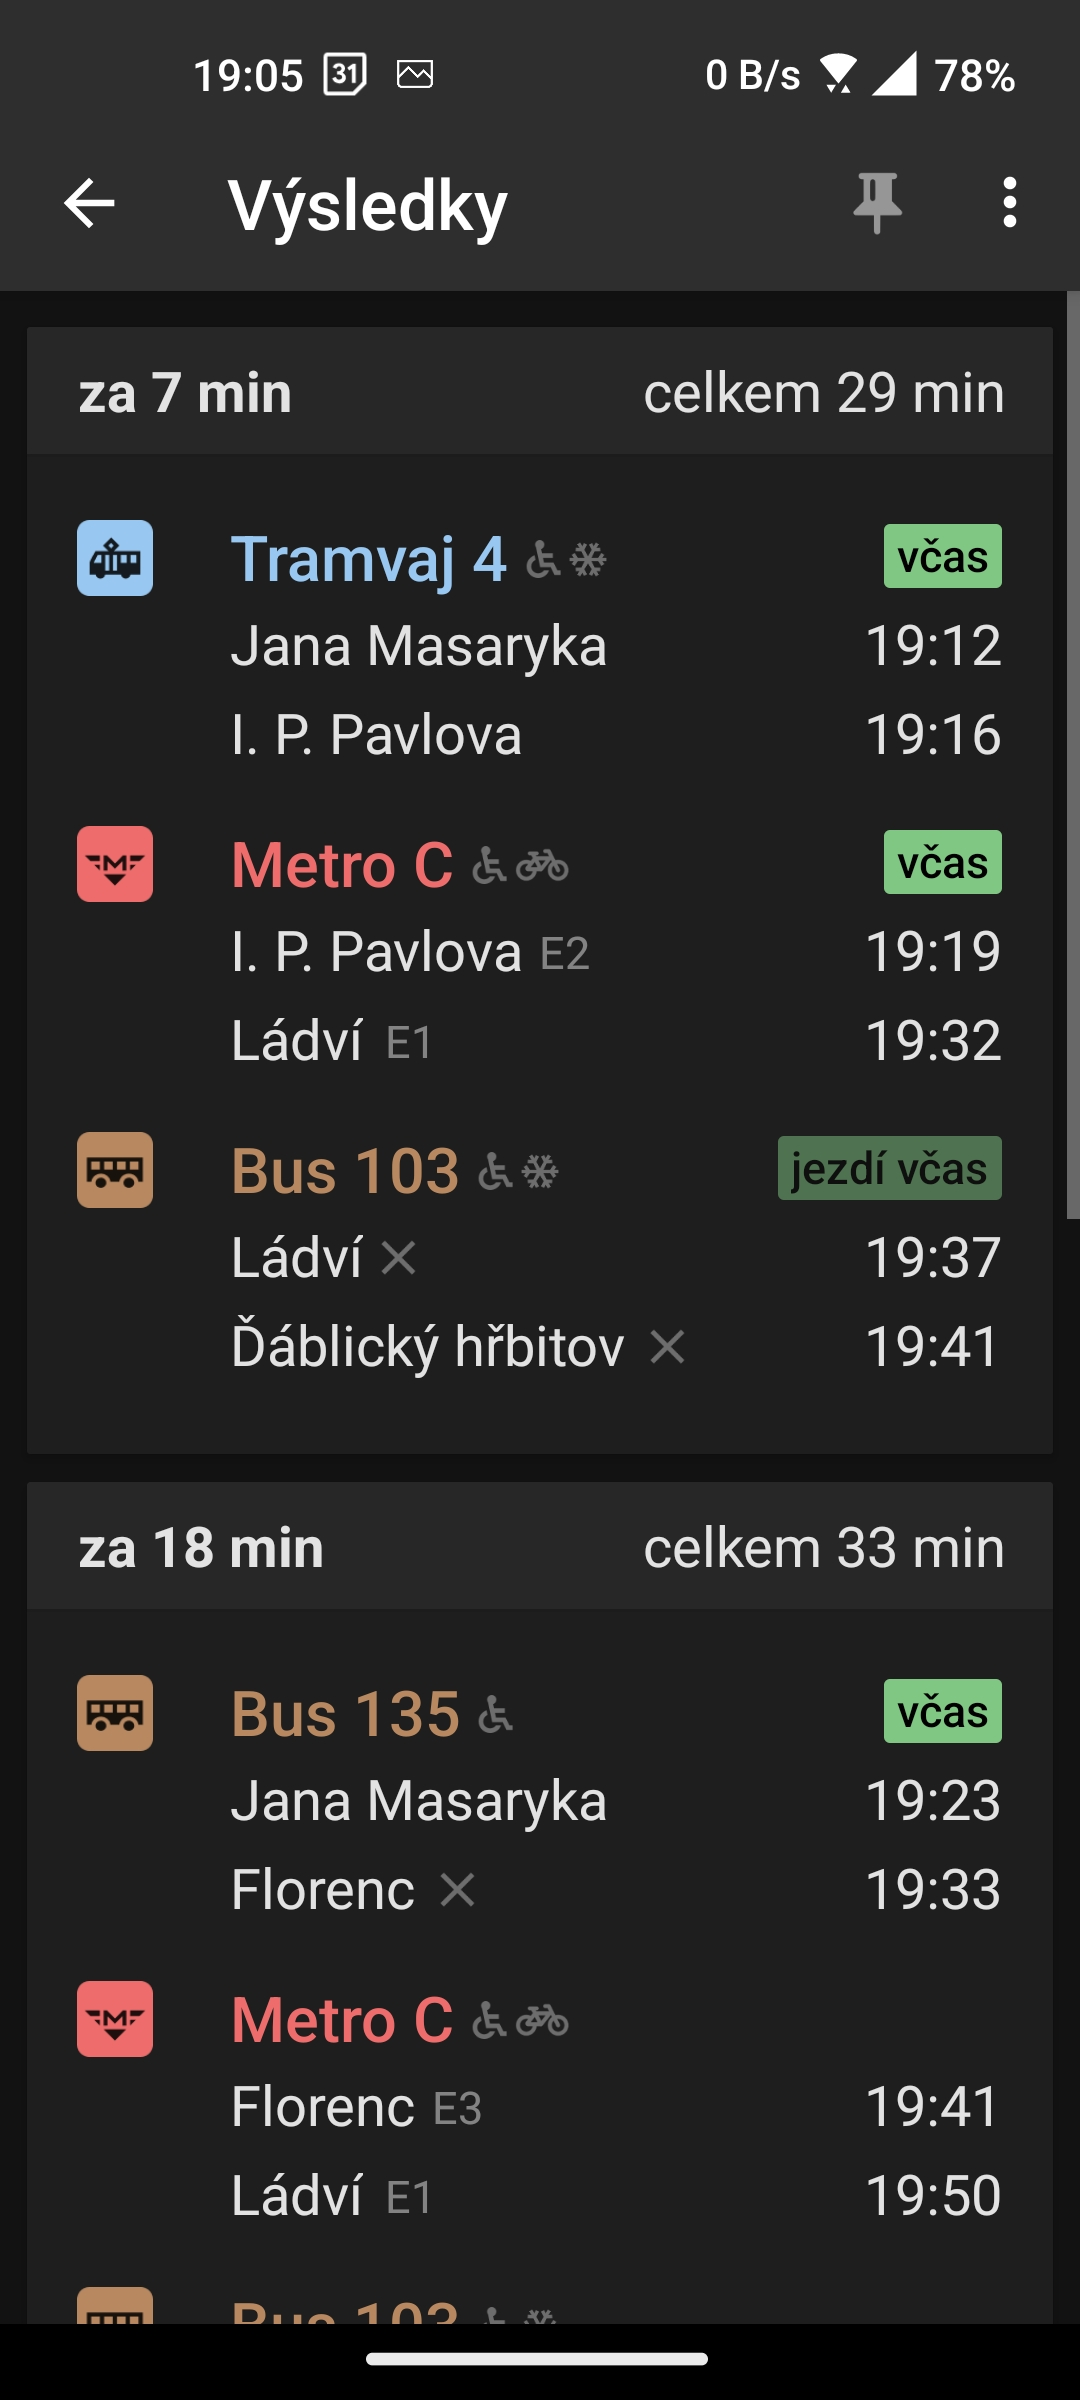
\includegraphics[width=0.45\textwidth]{img/screenshots/pubtran_result.jpg}
    \caption{Result of a connection search in Pubtran}
    \label{fig:pubtran}
\end{figure}

\subsubsection{CG Transit}

The main focus of CG Transit is to provide connection searching while being offline. Additionally, the app also works well online and can use current delay data in the same way as the other apps. It also has some basic configuration options like direct searches, intermediate stops, wheelchair searches, setting global absolute transfer time length and maximum walking time. However, it does not support any more detailed comfort preference settings or setting own walking pace and bikesharing is also not included in the searches. The app uses the more intuitive user interface type similar to IDOS and Pubtran (\cref{fig:cg_transit}).


\begin{figure}[h!]
    \centering
    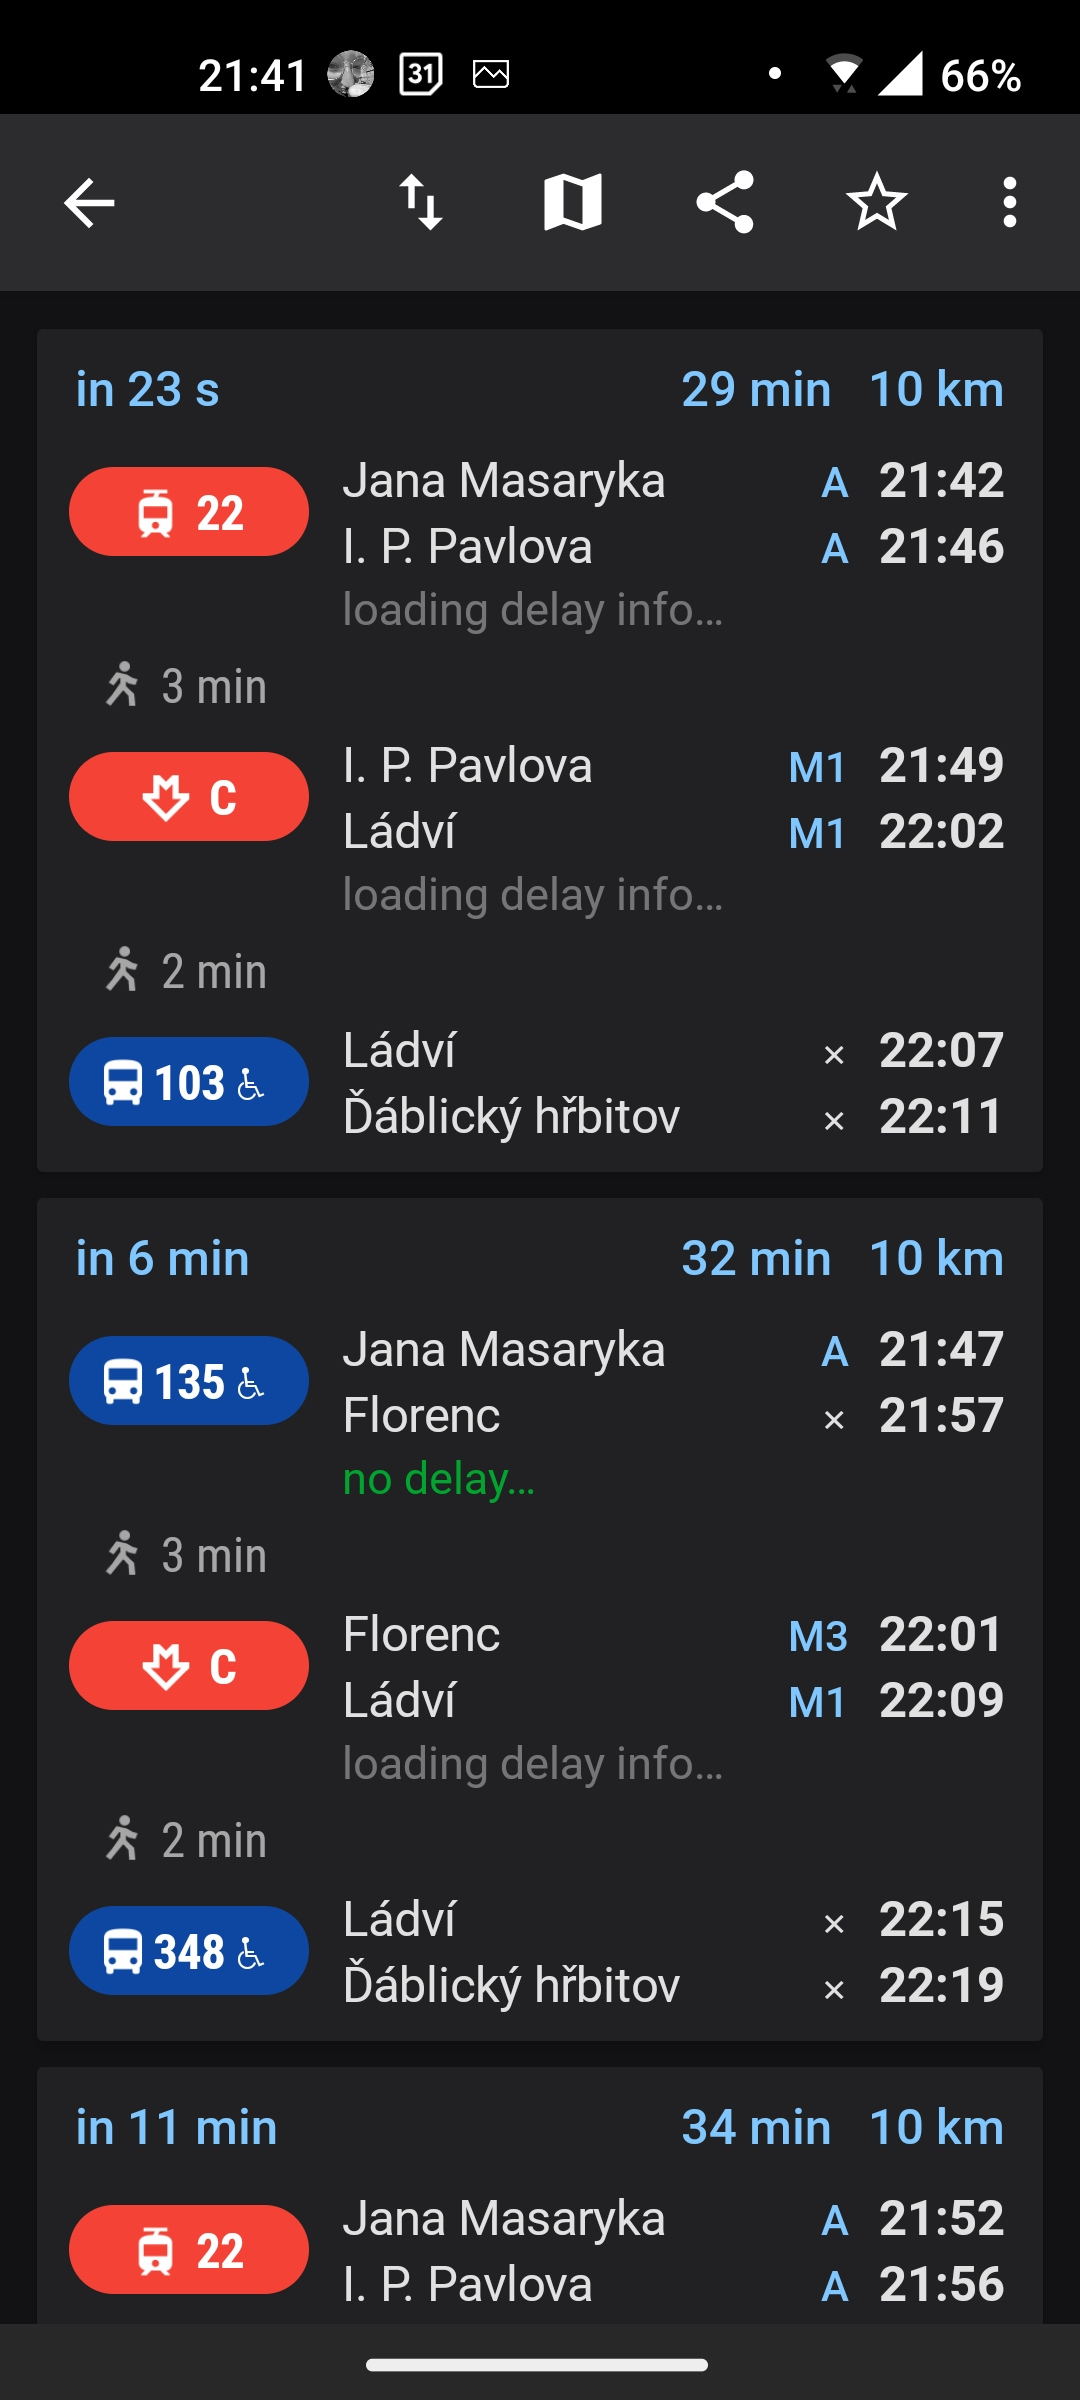
\includegraphics[width=0.45\textwidth]{img/screenshots/cg_transit_result.jpg}
    \caption{Result of a connection search in the CG Transit app}
    \label{fig:cg_transit}
\end{figure}

\subsection{Prague-specific solutions}

\subsubsection{PID Lítačka}

PID Lítačka is the official public transit application developed by the city of Prague. Its main purpose is ticket and transport pass management, but it also includes extensive connection search functionality. The app can be used in 2 modes, classic and advanced. In comparison to the other apps, even in classic mode (which only uses public transport and does not support bikesharing or other modes of transport) the configuration options are much more extensive. There is the option of setting maximum walking distance, maximum transfer count and walking pace (although there are only 3 possible values for Slow, Normal and Fast). It can also search for wheelchair-accessible or low-floor connections. The advanced mode (which at the moment of writing this thesis is in Beta) provides extensive support for other modes of transport, such as own bike or car or shared bikes, scooters, motorcycles, cars and taxis. 

All of this multimodal functionality was added to the app fairly recently and only after the work on this thesis was begun. But, while this has hindered the intent for the subject of this thesis to be the first app supporting bikesharing inclusion in Prague's public transit connection searches, there still remains room for improvement. Specifically, as opposed to the classic mode which displays the results in a very intuitive and clear form similar to that of IDOS and Pubtran (\cref{litacka_classic}), the advanced mode, due to its inclusion of a broad spectre of transport modes, displays the results in a much less intuitive form similar to those of Maps Google and Moovit (\cref{litacka_advanced}). While in this case it doesn't group the resulting connections by their structure (i.e. lines/routes taken) and instead displays the individual connections, it still provides the user with much less information on where the individual connections will take them through. As our app is targeted to audience that already has experience with Prague's public transit system, the users are expected to be able to use their experience to select the percieved best connection out of the presented results. For example, they might know from experience that in a particular section, a line often gets stuck in traffic or gets very crowded, and they can use this information to select other connections from the list of results. In PID Lítačka's advanced mode, this is made much harder by hiding each connection's route information behind a through-click. 


\begin{figure}[h!]
  \begin{subfigure}{.45\textwidth}
  \centering
    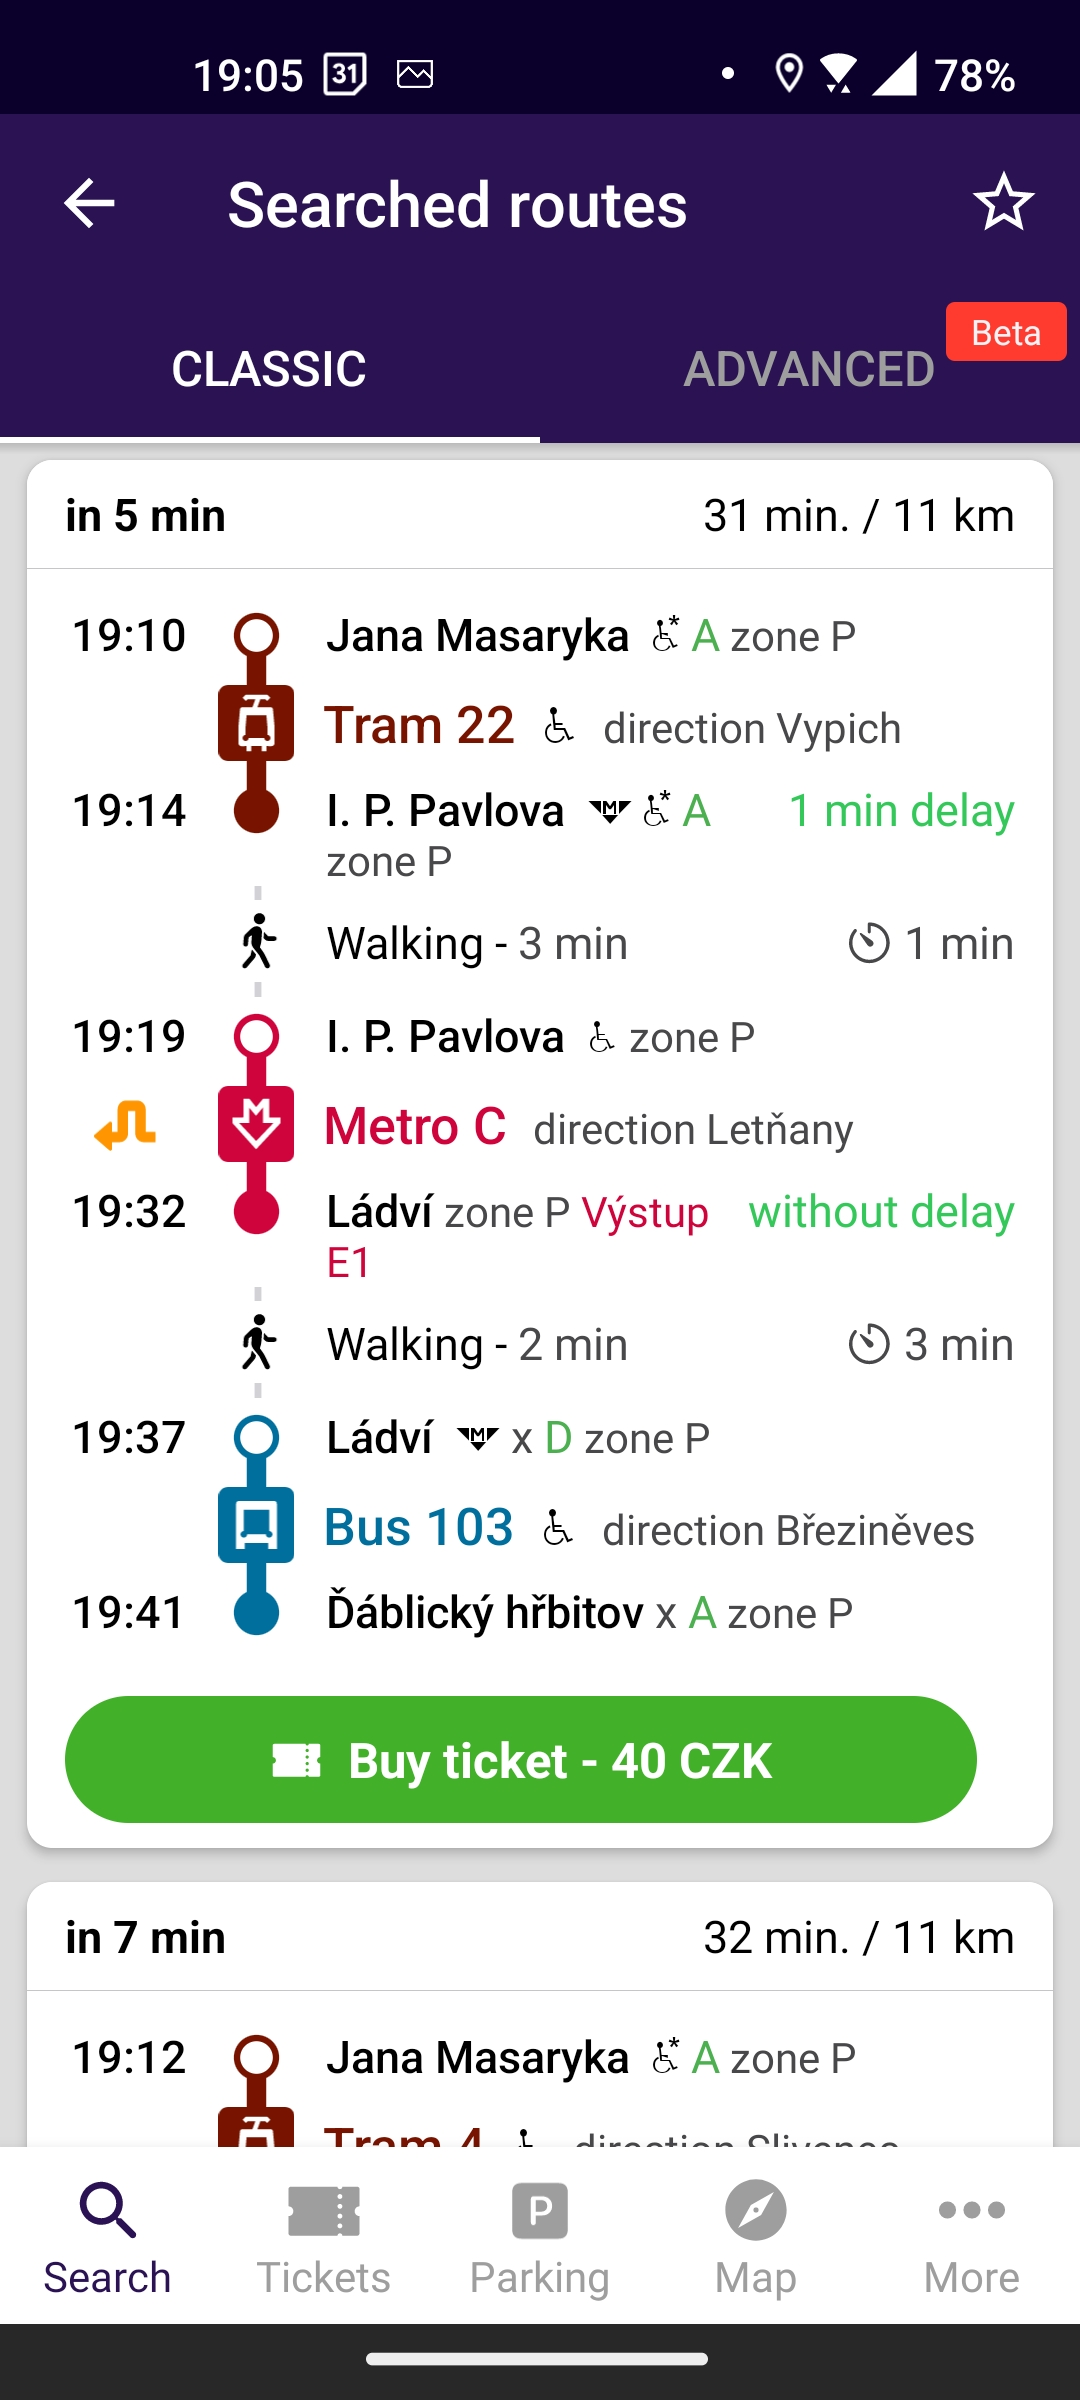
\includegraphics[width=\linewidth]{img/screenshots/pid_litacka_result_simple.jpg}
    \caption{Classic mode}
    \label{litacka_classic}
  \end{subfigure}%
  \hfill
  \begin{subfigure}{.45\textwidth}
  \centering
    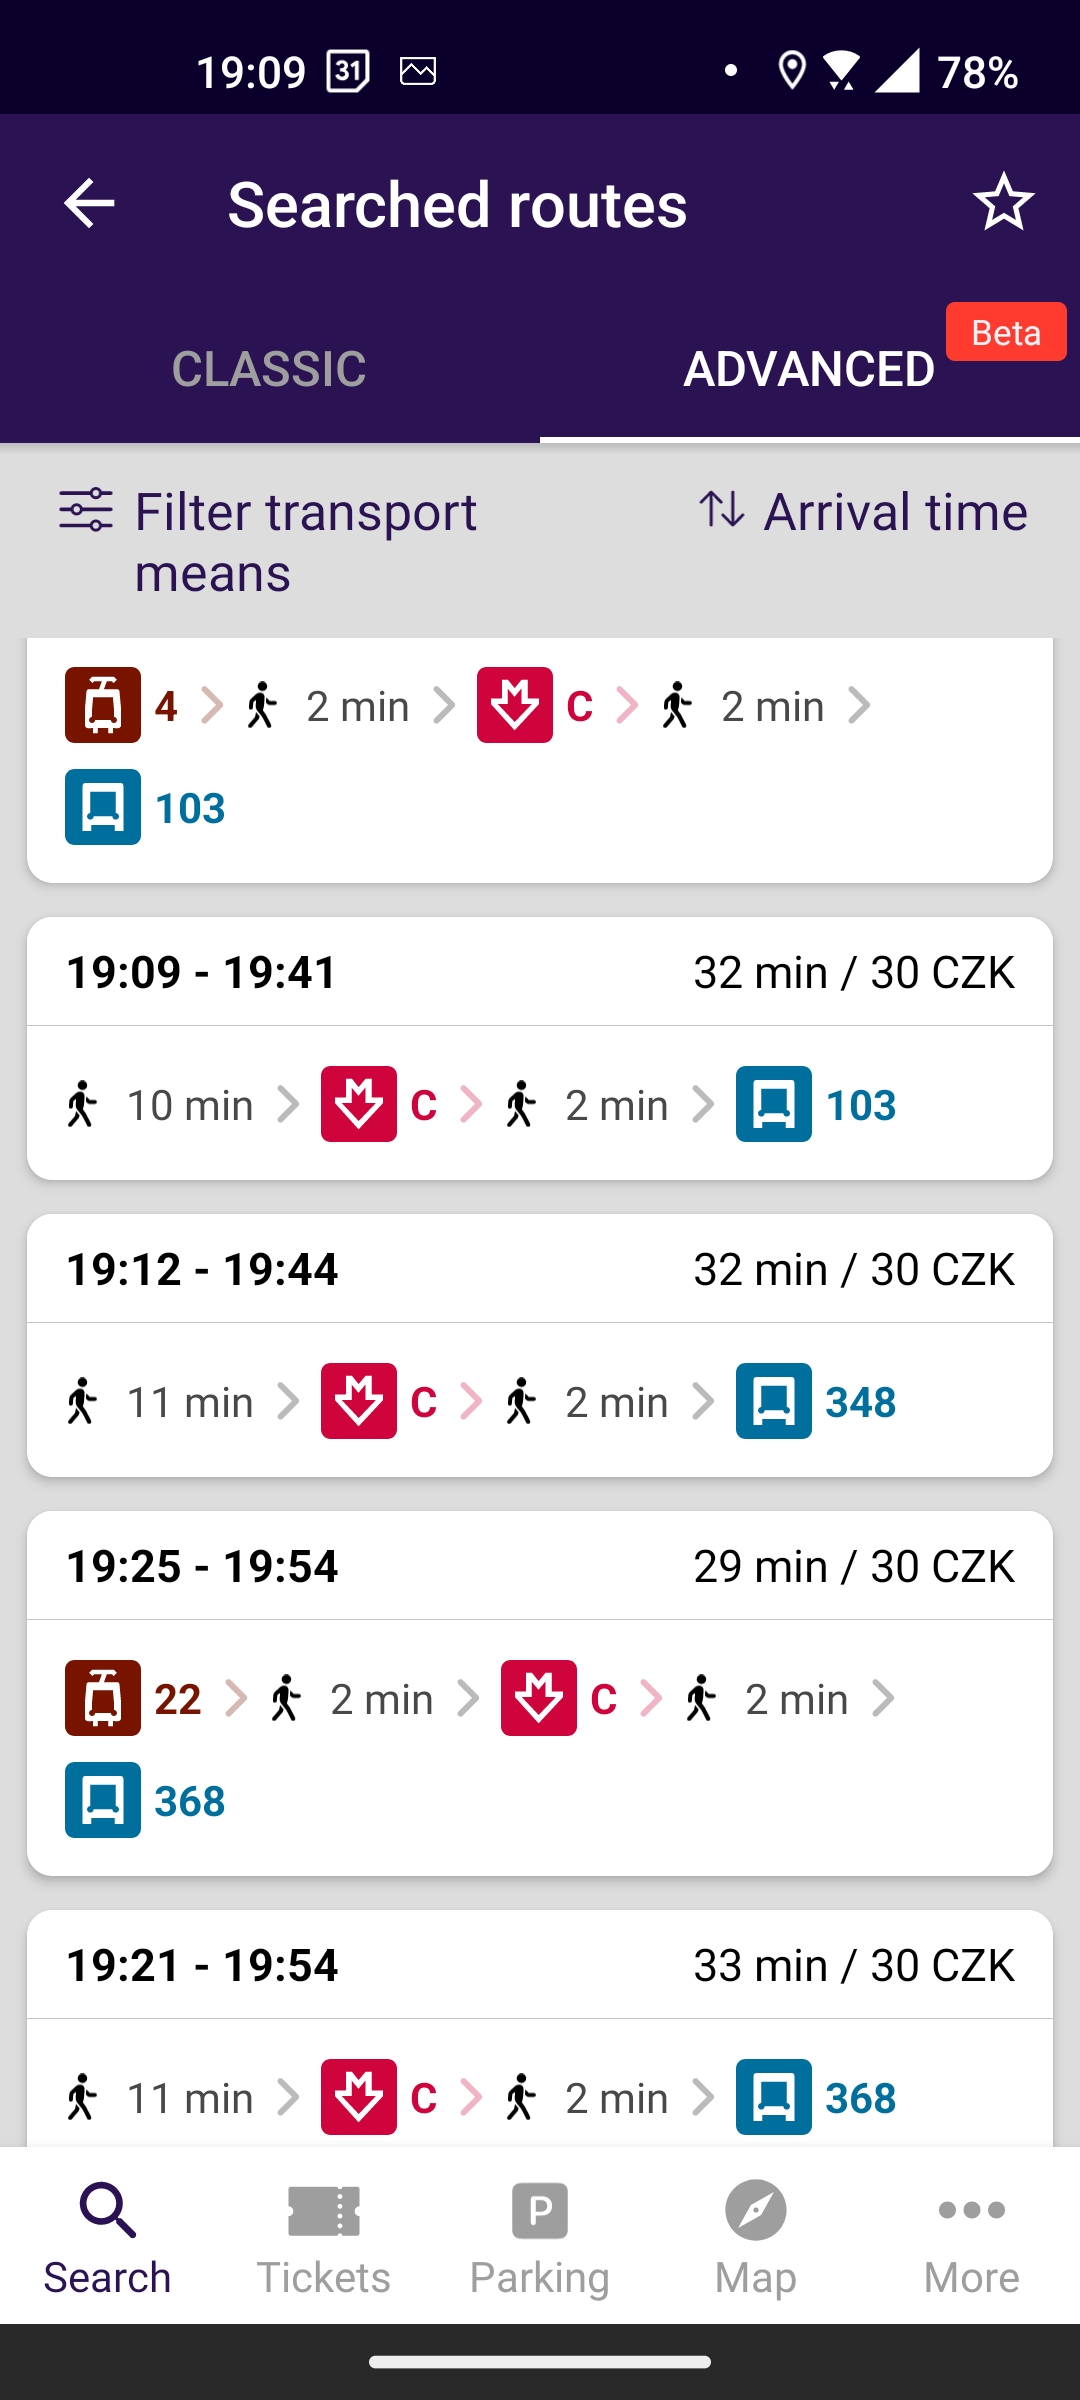
\includegraphics[width=\linewidth]{img/screenshots/pid_litacka_result_extended.jpg}
    \caption{Advanced mode}
    \label{litacka_advanced}
  \end{subfigure}
  \caption[Comparison of search results in PID Lítačka]{Comparison of search results in PID Lítačka: (a) classic mode and (b) advanced mode}
  \label{litacka}
\end{figure}

\subsection{Other solutions}

There are also other applications we have not included in this overview, such as the official connection search website of Prague's main transport company\footnote{https://spojeni.dpp.cz/} or the Mapy.cz map application from Seznam.cz\footnote{https://mapy.cz/}. However, neither of these solutions exists in the form of a dedicated mobile app. As for most people a mobile application is the go-to way of searching for public transit connections, our goal is to develop such a dedicated application and we thus do not include solutions that only work in the form of a website.

\subsection{Takeaways from the existing solutions}

Although every app we introduced is different, we can observe some larger trends. For example, the applications are divided in terms of the way they display the results. While some apps display only the structure of the connections together with the used lines' names and some even group the resulting connections into groups according to their structure, other apps display each connection separately while showing not only the line names, but also the specific stops at which the individual trips within the connection get boarded and disembarked. While the first approach requires less screen space and can provide a better overview of all the ways one can travel between the two points, the second approach is better suited to the use case our app is designed for, i.e. searching for a connection within one relatively small and dense city. This is because with this approach, the user can have a better overview of what routes are available at the particular time they need to travel and even more importantly, they can use the additional routing information to select the best option out of the list of results according to their past traveling experience.



Before building our app, we can analyze the features of the existing solutions and select those that contribute most to the goals we set out for our app. As the intended audience for our app are people who use Prague's public transit as a daily tool to get around the city, our goal is to provide them with the option to provide additional input into the connection searches, which will enable them to get better personalized results.

For example, the option to set one's walking (and possibly cycling) pace will improve the relevance of their results, as the durations of transfers and bike trips will better correspond to their habits and preferences, leading to more precise and tailored results. However, even though the user would be able to set their walking pace, there may be situations where they wouldn't be able to walk at their standard pace, such as when transporting heavy luggage or traveling with their older relatives. It would be impractical to assess and change the pace for every connection search. Instead, it would be useful to have the option to set a transfer time buffer value. This could for example be implemented as a simple slider that would be easy and quick to operate before any search that would need it.
The ability to set the maximum length of a transfer would also help to make the results more personalized, as in some situations, the user may prefer not having to perform longer transfers, even if that would mean that the connection would be shorter in time.
While some of the existing apps offer some of these features, none provides all of them in a way that would be usable on a day-to-day basis.

Furthermore, as mentioned above, on two separate occasions, one person may use public transit for two very different things. For instance, when someone is traveling to a work meeting or a school lecture, they will probably want to use the fastest connection. If they are in a big hurry, they might even want to use more transfers than strictly necessary or risk using very short ones, if it means they will be able to get to their destination quicker. On the other end, there may be situations where the same person needs to travel to the airport or railway station with a lot of luggage. In this case, time may not be the limiting factor. Instead, they might want to take the most comfortable route that takes them to their destination using the least possible transfers. Most existing solutions only offer a simple toggle for only searching for direct connections or only setting the absolute maximum number of used trips. Thus, we would like our app to have a more efficient support for specifying the balance between minimizing time and minimizing the number of necessary transfers.

Many of the apps are also able to display current delay information, but do not include it within the connection search algorithm itself. This means that they can suggest connections that are not possible to make due to one of the trips being delayed too much. There is no point in showing such results to the user.

On another note, including bikesharing services within the connection search will lead to users having more options to choose from when traveling through the city. Using shared bikes can often be a faster and/or more pleasant alternative to taking public transit. Also, the city of Prague currently provides bikesharing rides of up to 15 minutes as part of the public transit tickets, so it would also be helpful to be able to limit the maximum length of bike trips to fit in this time frame.

These are just some of the features that some of the mentioned apps (partially) provide, and which we would like to include in our application. To provide a better overview, we present the comparison between the features of the existing solutions and those of our application in the table below. The detailed meaning of each feature is described within the app requirements below the table.

\subsection{Comparison of the different solutions}


\overfullrule=0pt
\begin{table}[H]
\centering
\scriptsize % Set base font size to scriptsize
\begin{tabularx}{\textwidth}{ | >{\scriptsize\centering\arraybackslash}m{3.6cm} | >{\tiny\centering\arraybackslash}m{0.8cm} | >{\tiny\centering\arraybackslash}m{0.8cm} | >{\tiny\centering\arraybackslash}X | >{\tiny\centering\arraybackslash}X | >{\tiny\centering\arraybackslash}m{0.8cm} | >{\tiny\centering\arraybackslash}X | >{\tiny\centering\arraybackslash}m{0.8cm} | }
\hline
\textbf{Features\textbackslash Apps} & \textbf{Pubtran} & \textbf{IDOS} & \textbf{Lítačka} & \textbf{Google Maps} & \textbf{CG Transit} & \textbf{Moovit} & \textbf{PragO} \\ \hline
\textbf{Time/Comfort balance setting} & \textcolor{red}{NO}\footnotemark[1] & \textcolor{red}{NO}\footnotemark[1] & \textcolor{orange}{NO}\footnotemark[2] & \textcolor{darkyellow}{PARTLY}\footnotemark[3] & \textcolor{orange}{NO}\footnotemark[2] & \textcolor{darkyellow}{PARTLY}\footnotemark[3] & \textcolor{green}{YES} \\ \hline
\textbf{Adjusting transfer time buffers} & \textcolor{red}{NO} & \textcolor{red}{NO} & \textcolor{green}{YES} & \textcolor{red}{NO} & \textcolor{red}{NO} & \textcolor{red}{NO} & \textcolor{green}{YES} \\ \hline
\textbf{Maximum walking distance} & \textcolor{red}{NO} & \textcolor{red}{NO} & \textcolor{green}{YES}\footnotemark[5] & \textcolor{darkyellow}{PARTLY}\footnotemark[8] & \textcolor{green}{YES}\footnotemark[7] & \textcolor{green}{YES}\footnotemark[7] & \textcolor{green}{YES} \\ \hline
\textbf{Includes bikesharing in searches} & \textcolor{red}{NO} & \textcolor{red}{NO} & \textcolor{green}{YES}\footnotemark[4]\footnotemark[5] & \textcolor{red}{NO} & \textcolor{red}{NO} & \textcolor{red}{NO} & \textcolor{green}{YES} \\ \hline
\textbf{Custom walking/cycling pace} & \textcolor{red}{NO} & \textcolor{red}{NO} & \textcolor{darkyellow}{PARTLY}\footnotemark[6] & \textcolor{red}{NO} & \textcolor{red}{NO} & \textcolor{darkyellow}{PARTLY}\footnotemark[6] & \textcolor{green}{YES} \\ \hline
\textbf{Ability to start search from other nearby stops} & \textcolor{green}{YES} & \textcolor{red}{NO} & \textcolor{green}{YES}\footnotemark[4]\footnotemark[5] & \textcolor{green}{YES} & \textcolor{red}{NO} & \textcolor{green}{YES} & \textcolor{green}{YES} \\ \hline
\textbf{Delay included in planning} & \textcolor{red}{NO} & \textcolor{red}{NO} & \textcolor{red}{NO} & \textcolor{green}{YES} & \textcolor{red}{NO} & UNCLEAR\footnotemark[9] & \textcolor{green}{YES} \\ \hline
\textbf{Metro departure times displayed exactly} & \textcolor{red}{NO} & \textcolor{red}{NO} & \textcolor{red}{NO} & \textcolor{red}{NO} & \textcolor{red}{NO} & \textcolor{red}{NO} & \textcolor{green}{YES} \\ \hline
\textbf{Low data usage} & \textcolor{green}{YES} & \textcolor{green}{YES} & \textcolor{green}{YES} & \textcolor{red}{NO} & \textcolor{green}{YES} & \textcolor{red}{NO} & \textcolor{green}{YES} \\ \hline
\end{tabularx}
\caption{Comparison of features between different apps}
\label{tab:apps_comparison}
\end{table}


\footnotetext[1]{Only provides normal or direct searches}
\footnotetext[2]{Only provides maximum transfer count setting}
\footnotetext[3]{Has no option for absolutely fastest connections, only for "Best Route"}
\footnotetext[4]{Only in Advanced mode, which is currently still in Beta version}
\footnotetext[5]{Feature only introduced after work on this thesis was begun}
\footnotetext[6]{Only 2-3 discrete options (Slow, Normal, (Fast)) - no option to set exact pace}
\footnotetext[7]{Set in minutes, not meters}
\footnotetext[8]{There is only a "Less walking" option}
\footnotetext[9]{The app's UI displays for every trip the first few available options regardless on whether they are reachable by the previous trips of the connection. Due to this, it is unclear whether the delay is included in the planning}


As you can see, most existing apps have very limited possibilities in terms of search personalization options. The only notable exception in this direction is the PID Lítačka app developed by the city of Prague, which added many of the desired features during the last year. Most notably, they recently included bikesharing services within their connection searches, which is a feature that none of the other apps have included yet. However, many of these features were only added after work on our application has commenced, and some features are still missing or implemented only partially. Thus, we set out to implement our own application that would include all of the useful features we mentioned above and would thus be best suited for our target audience. In particular, we set out to fulfill the following requirements:

\newpage

\section{Requirements}

In this section, we present both the functional and qualitative requirements we set out to fulfill with our application. We will introduce the functional requirements in the form of user stories - these are short stories describing \textit{who} wants/needs \textit{what} functionality from the application and \textit{why} they want/need it.

\begin{enumerate}
\renewcommand{\labelenumi}{\textbf{R\arabic{enumi}}}
\item The user can use the application to find public transit connections in the PID network between two stops of given names, so that they can find the best way to get to their desired destination
\label{req:finds_connection}

\item The user can also find public transit connections using their current location as the starting point, so that they don't need to remember the name of each of the stops near them and don't have to select a single one as the start.
\label{req:src_by_coords}

\item The user can search for a connection by providing the earliest possible departure time from the starting point, or the latest acceptable arrival time at the destination point. This is to support both situations where the user is currently at point A and wants to get to point B as soon as possible, and where the user needs to arrive at point B at a certain time and wants to find out at what time they need to set out.
\label{req:arr_dep_time}

\item The user can set their own walking pace that will be used for calculating transfer times, so that the results better reflect their abilities.
\label{req:walking_pace}

\item The user can adjust this walking pace on a search-to-search basis via a transfer buffer setting, so that they can both allow riskier transfers when they are in a hurry and increase the buffer when they are in a situation where they cannot walk at their normal pace.
\label{req:transfer_buffer}

\item The user can set the maximum allowed transfer distance, so that they can limit the distance that they would need to walk in situations where they prefer not to walk too far.
\label{req:max_transfer_distance}

\item The user can set the balance between prioritizing shortest possible time and least possible transfers, so that they can adjust the search to better reflect their current needs and preferences.
\label{req:comfort_balance}

\item The user can set the application to include shared bikes in its search algorithm, so that they can see when it might be better to perform a part of the connection on a shared bike instead of taking public transit trips.
\label{req:shared_bikes}

\item The user can set the maximum time of a bike trip to 15 minutes, so that the trip can be included as part of their public transit subscription and they do not have to pay for it themselves.
\label{req:bikes_max_15}

\item The user can set their own cycling pace that will be used for calculating bike trip times, so that the results better reflect their abilities.
\label{req:cycling_pace}

\item The user can adjust the cycling pace on a search-to-search basis via a bike trip buffer setting, so that they can both allow riskier connections when they are in a hurry and increase the buffer when they want to take their time.
\label{req:bike_trip_buffer}

\item The user can set the time it takes them to lock and unlock a shared bike, so that the results better reflect their habits and abilities.
\label{req:lock_unlock_time}

\item For every displayed bike trip, the application will show the user the number of free bikes currently available at its source bike station, so that the user has a better overview of their chances to make the trip.
\label{req:bike_count}

\item If the user sets the source/destination stop name to a specific name, the application will still allow connections starting/ending at other nearby stops. This helps the user in situations where there are multiple different stops nearby served by different routes. It prevents the user from having to run the search for each of the possible source/destination stops separately.
\label{req:multiple_src_dest}

\item When the user puts in the name of the source or destination stop, the application will provide them with relevant existing stop name suggestions from which they will be able to choose, so that they do not have to spend more time by typing out the whole exact name.
\label{req:stop_name_suggestions}

\item The departure and arrival times are displayed to the user exactly in seconds, especially in the metro. This is to provide the user with exact information on how long they have for a transfer, as in the metro, there is a big difference between a 35 seconds and a 85 seconds long transfer, both of which could be rounded to 1 minute.
\label{req:exact_times}

\item The application will show multiple different results to the user, so that they can easily select the one that suits them the best.
\label{req:multiple_results}

\item The user can for any used trip in any of the resulting connections display earlier or later alternative trips, so that they know what other alternatives they can take should they not be able to make the one trip the application suggested.
\label{req:trip_alternatives}

\item For every displayed resulting connection, the application will show the time left until the connection starts. If the connection starts with a walking transfer, it will display both the time left until the user should start walking and the time left until the first trip of the connection leaves. This is so that the user has exact information on when they should leave to make the connection.
\label{req:countdown}

\item For every trip of every connection, the application will show its current delay, so that the user can have better overview of the current situation within the city.
\label{req:delays}
\end{enumerate}


Apart from these functional requirements, we also want to fulfill a few qualitative requirements. These specify how the system performs certain functions and what qualities it needs to have while providing the functionality described above. These include the following:

\begin{enumerate}
\renewcommand{\labelenumi}{\textbf{R\arabic{enumi}}}
\setcounter{enumi}{20}
\item The application will include and use the delay information during the search and not only add this information to the (already created) results. This is to prevent it from presenting connections to the user that are not viable due to the current delay situation.
\label{req:delays_included_in_search}

\item The application needs to keep a relatively low data consumption, to save the user's data consumption. In specific terms, it may not send or receive more than 100kB of data per connection displayed.
\label{req:low_data}

\item When running the server on a typical modern machine, the response time for at least 90\% of requests needs to be lower than 1 second. This is to prevent users from having to wait too long for their results.
\label{req:response_time}
\end{enumerate}



\section{Available data}

Our application will need multiple different types of publicly available data to function properly. Firstly, it will need data describing Prague's public transit network with its routes, trips and stops. Secondly, to provide the users with the current delay information and to be able to include it in connection searches, it will need to source this live delay data and to update it frequently. Lastly, it will also require data about the bikesharing networks in Prague to include bikesharing in the searches. To be able to calculate bike routes throughout the city, it will also need some map data of the area covered by the bikesharing providers.

\subsection{Public transit network data}

The transportation agency of the city of Prague publishes the static data describing its public transit network in the GTFS (General Transit Feed Specification) format. This is the industry standard used by transit agencies around the world to provide their data to trip planners, researchers, policy makers, and other third-party apps\cite{gtfs2024}.

The data is available to download from the city website\footnote{http://data.pid.cz/PID\_GTFS.zip} in zip format. The archive contains a total of 20 files, but for our purposes we will only need some of them. In particular, the most important files for our application are \texttt{stops.txt}, \texttt{stop\_times.txt}, \texttt{trips.txt}, \texttt{routes.txt}, \texttt{calendar.txt} and \texttt{calendar\_dates.txt}. In this section, we will take a look at how the data is structured, how the files are linked together and what that means for our application.

\begin{figure}[h!]
    \centering
    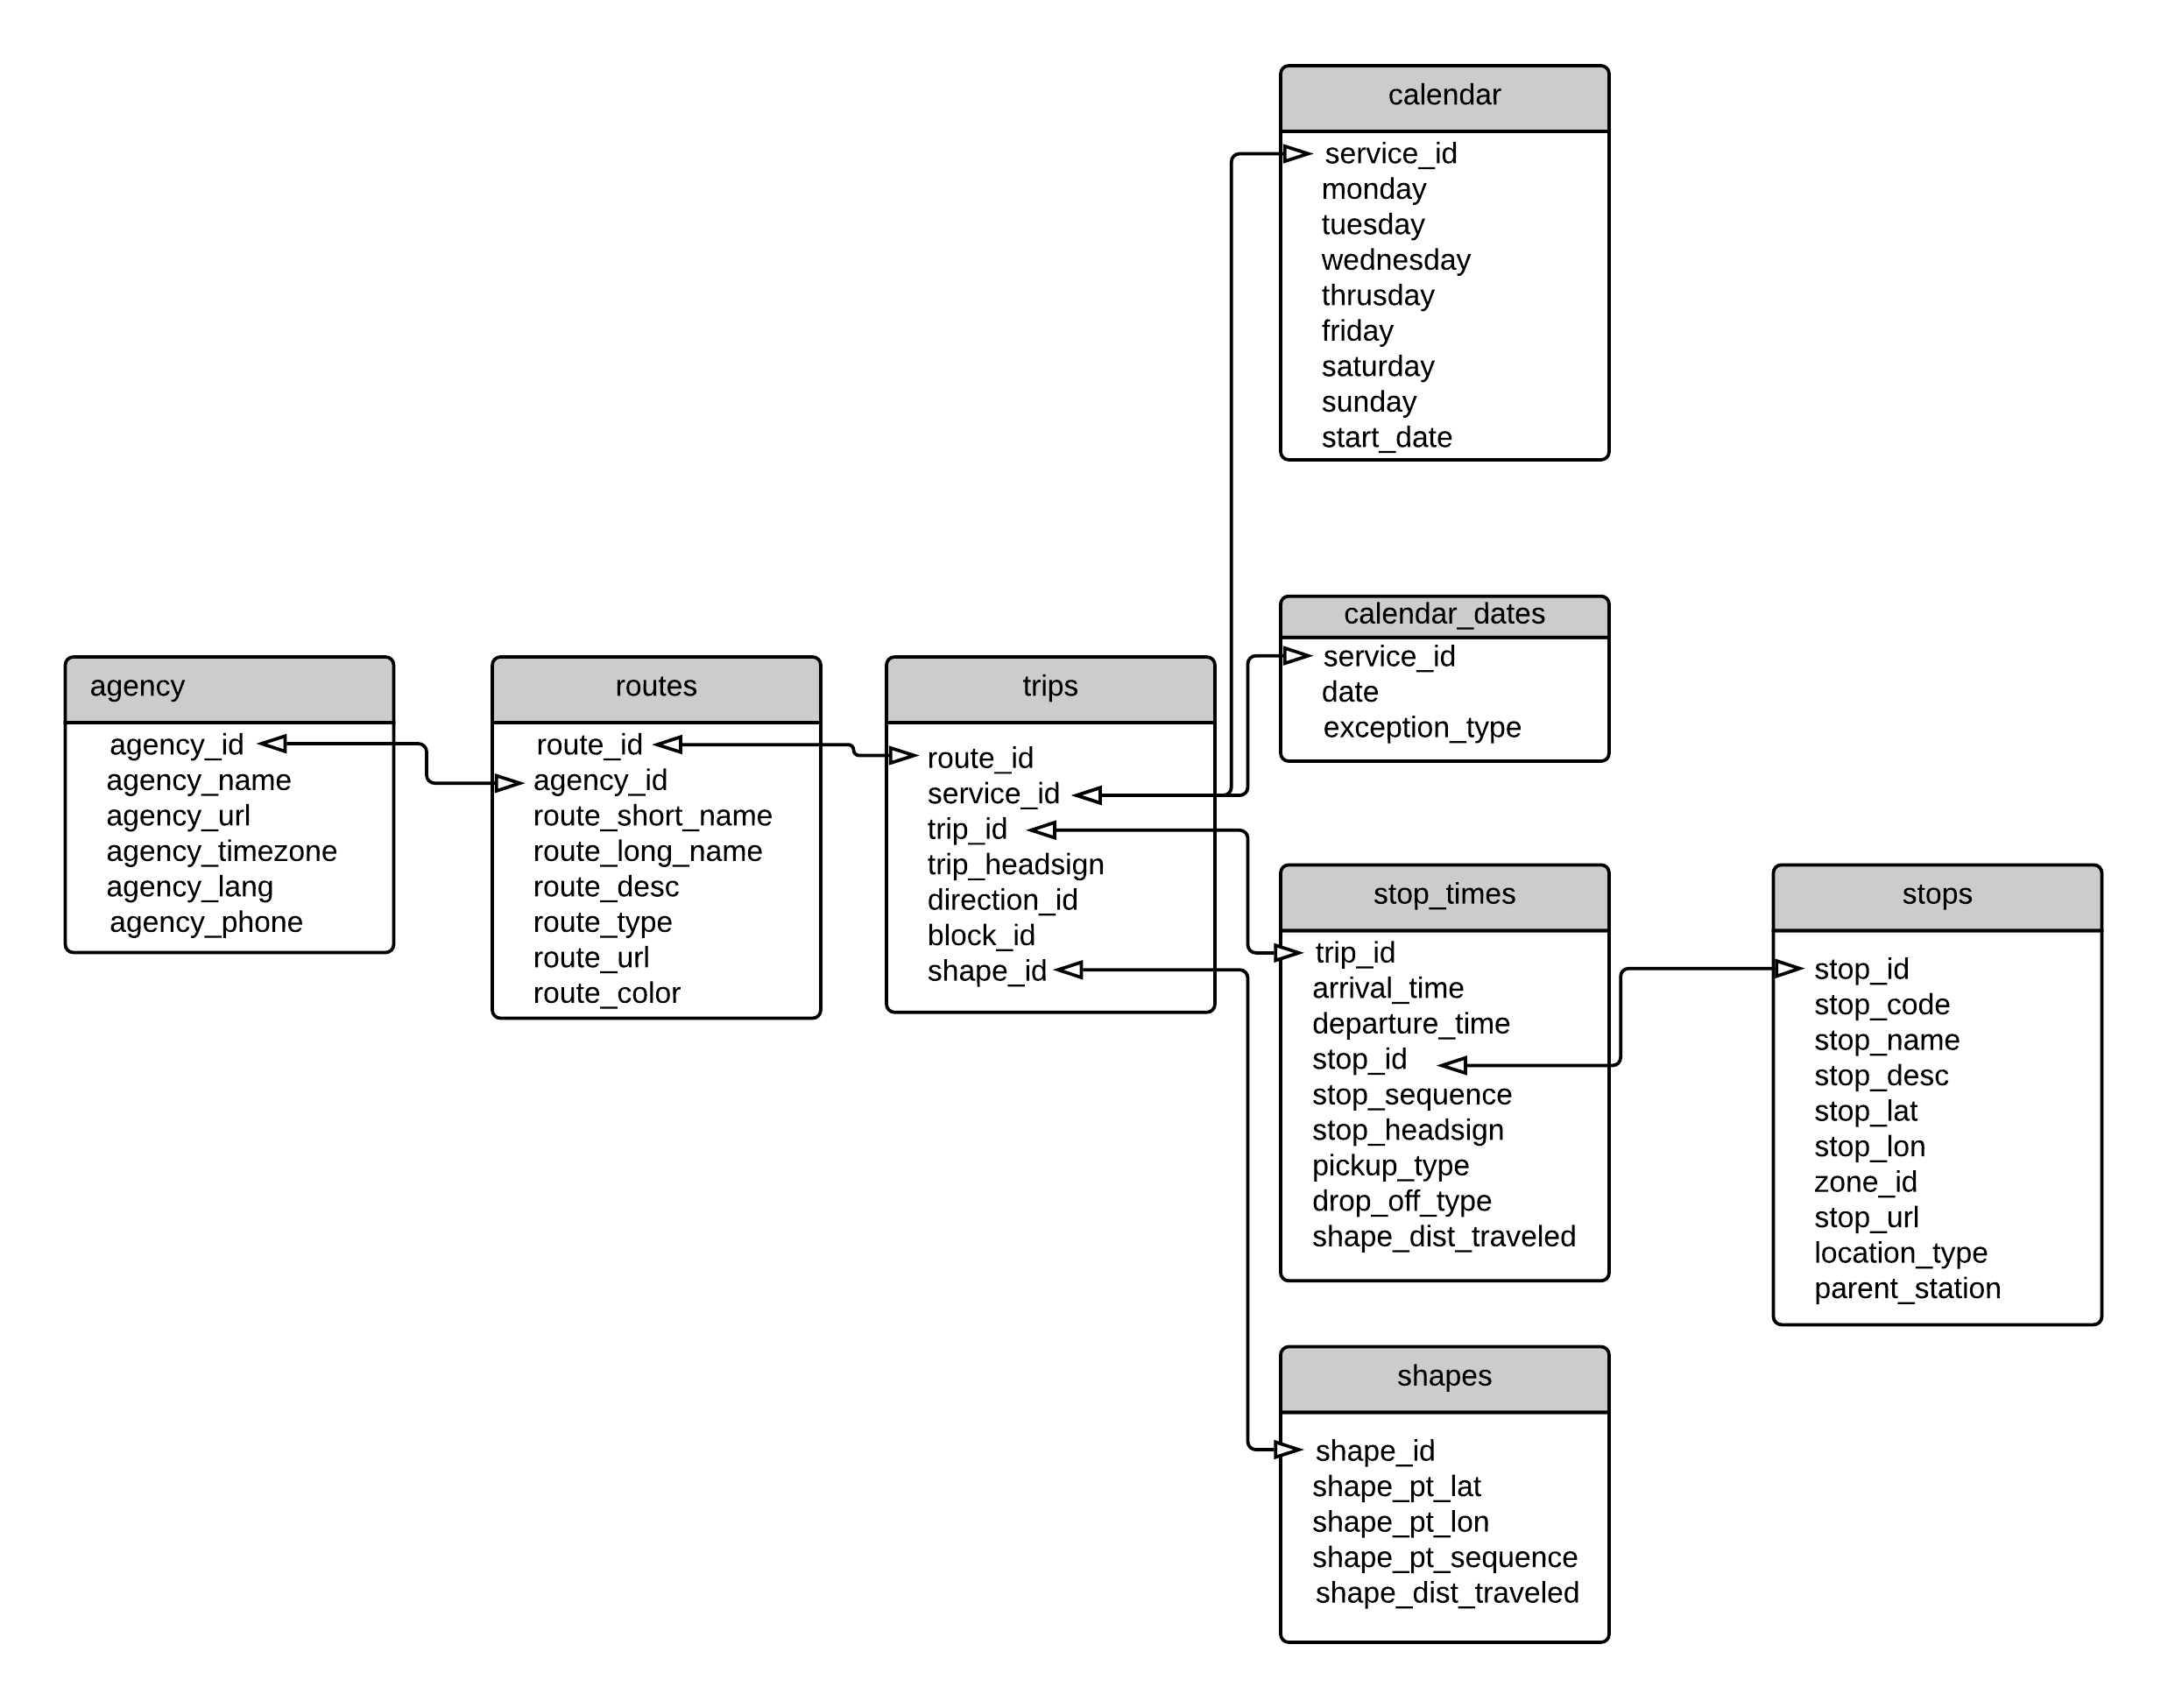
\includegraphics[width=\textwidth]{img/gtfs_scheme.png}
    \caption[GTFS Format Scheme]{GTFS format scheme. Source: Pereira, Andrade and Vieira\cite{pereira2023gtfs}.}
    \label{fig:gtfs_scheme}
\end{figure}

\begin{itemize}
    \item \texttt{stops.txt}
    
    This file contains detailed information about all stops within the network, containing one line per every stop. For our purposes, the most important data within this file are the ids (\textit{stop\_id}), names (\textit{stop\_name}) and the coordinates (\textit{stop\_lat} and \textit{stop\_lon}) of the stops. It also contains information such as what tariff zone the stop is in, an URL of the stop's website or whether the stop is suitable for wheelchair users. However, for our application we will not be using this additional data.

    \item \texttt{routes.txt}

    This file contains information about all the lines within the network. In particular, for every route it holds information about its id (\textit{route\_id}, its short and long names that riders use to identify the route (\textit{route\_short\_name} and \textit{route\_long\_name}, and the type of vehicle that serves the route (\textit{route\_type}). As described earlier, in the context of this thesis, we use the term \texttt{Route} to describe a single variation of a real-world line with its own list of stops. However, one line of the file corresponds to one real-world public transit line, not to one \texttt{Route}. We will construct the individual \texttt{Routes} during the parsing stage by combining the data from this file with the data from the \texttt{trips.txt} and \texttt{stop\_times.txt} files.

    \item \texttt{trips.txt}

    This file contains information about all the trips within the network. Every trip references a single line from the \texttt{routes.txt} file. It also has its own id (\textit{trip\_id}), through which a trip is referenced in the \texttt{stop\_times.txt} file. Finally it contains a \textit{service\_id}, which refers to an entry within the \texttt{calendars.txt} and \texttt{calendar\_dates.txt} files. The other information like the trip's headsign will not be used by our application.

    \item \texttt{stop\_times.txt}

    This is typically the largest file in the archive, as it holds most of the useful information about trips and their stop times within the network. It contains a single line per every stop of every trip. The trip is referenced via the \textit{trip\_id} property. The stop is referenced via the \textit{stop\_id} property. It contains both the time of arrival (\textit{arrival\_time}) and departure (\textit{departure\_time}) of the trip at the stop. It also contains the stop's index within the trip's stop list (\textit{stop\_sequence}). The other information will not be necessary for our purposes.

    \item \texttt{calendar.txt}

    As the \texttt{stop\_times.txt} file only contains times and not dates of the trips' stops, this information needs to be present somewhere else. Via the \textit{service\_id} property, each line of this file specifies the dates at which the trip with that \textit{service\_id} is active. It does this by providing start and end dates of the time frame (\textit{start\_date} and \textit{end\_date}) and boolean values specifying on what days of the week between the dates the trip is active (\textit{monday} - \textit{sunday} properties).

    \item \texttt{calendar\_dates.txt}

    This file specifies exceptions to the rules within the \texttt{calendar.txt} file. Every line is once again indexed by a \textit{service\_id} and it contains a \textit{date} and \textit{exception\_type}, which specifies whether this is a positive or negative exception (i.e. whether it has been added or removed for the speciffied date).

    \item Other files

    There are also many additional files with data describing fares, fare zones, guaranteed transfers, metro and train station pathways and trip paths, which our application does not use.
\end{itemize}

In Prague, this data is updated daily between approximately between 4:00 and 4:30\cite{pidopendata}. It's validity is typically around one to two weeks, but partial changes may happen every day. Thus, our application needs to refresh this data every day to stay up to date.

\subsection{Delay data}

To provide users with current information about delays within the network and to use this data to provide more relevant results, we will need to be able to source this dynamic real-time data periodically from a GTFS Realtime data source. This is again a format designed specifically for this purpose. As opposed to the GTFS Static format described above, this data is not provided in text form. Instead, it is available as a protocol buffer\cite{gtfs2024}, which is Google's language-neutral, platform-neutral and extensible mechanizm for serializing structured data\cite{protobuf2024}. This data is available through an official API of the city of Prague\footnote{https://api.golemio.cz/pid/docs/openapi/}. A total of 3 files are provided - \texttt{trip\_updates.pb}, \texttt{vehicle\_positions.pb} and \texttt{alerts.pb}, which contain information on current delays, real-time positions of public transit vehicles and current disruptions within the network respectively. Prague also provides a \texttt{pid\_feed.pb} file, which is just the first 2 files combined into one feed.

As we are only interested in the time values of delays within the network and do not need information on exact GPS coordinates of every trip, the only file relevant to our application is the \texttt{trip\_updates.pb} file. In particular, it contains \textit{stop\_time\_updates} for every active trip, which specify the actual or expected stop times at the trip's stops. It also contains an experimental \textit{delay} field specifying the length of the current delay compared to the scheduled time. This is all the information we will need to implement delay handling within our application, and thus we won't be using the other provided data fields.

\subsection{Bikesharing data}

While the city of Prague has direct access to data about the bikesharing systems of the Rekola and Nextbike companies thanks to their contract with them, this contract prevents them from publishing this data directly through their API. Unfortunately, there is no way to publically access this data of the Rekola company, which prevents us from including it's bikes within our searches. Fortunately however, the Nextbike company publishes the data about all of their bike systems around Europe, so we can access the Prague-specific data from this API. Thanks to this, we only need to use the network id of Prague to access the data in GBFS format from their website\footnote{https://gbfs.nextbike.net/maps/gbfs/v2/nextbike\_tg/cs/<FILE\_NAME>}.

While the GTFS format standardizes data about public transit networks, GBFS (General Bikeshare Feed Specification) does the same for bikesharing providers who want to publish standardized data about their networks. As opposed to GTFS, which mostly uses a CSV-like format, the GBFS files use JSON\cite{gbfs2024}. Our application only will be using 2 of the provided files:

\begin{itemize}
    \item \texttt{station\_information.json}

    This file contains static information about the bike stations within the network. In particular, for every station there is a \textit{station\_id}, a \textit{name}, a location (\textit{lat} and \textit{lon}). There also is a lot of additional information, such as the type of the station, its opening hours or rental methods, which we will not be using, as this information is the same for all of Nextbike's stations within Prague. The stations also have a \textit{capacity} property, however, this does not seem relevant in Prague, as this capacity is not enforced in any way and can be exceeded freely, so we will not be using this value either.

    \item \texttt{station\_status.json}

    The main information contained within this file is the number of free bikes available at each station. Again, for our purposes we will only be using the \textit{station\_id} and \textit{num\_vehicles\_available} properties, as the other information is irrelevant in our setting.
\end{itemize}



\subsection{Map data}

As part of our application, we will need to implement bike routing within the city. In contrast to the public transit trips, the routes of which are directly specified within the data itself, for bikesharing services, we only have the list of stations and need to find the paths between them ourselves. One way to solve this problem would be to use an external routing API, such as the one from Mapy.cz, which provides this exact functionality\cite{mapyczapi}. However, such API's are typically paid, which would be problematic for calculating a large number of connections. Furthermore, as our application will not show the trips on a map, it only needs information about the trip's length and duration and not its exact path. Paying for getting the exact best route when we will not need it seems wasteful, and thus we decided to use our own routing.

As implementing the whole routing functionality would be way out of scope for this project, we have used a library for this purpose, which will be described in detail in following chapters. This library, like all other alternatives that provide this routing functionality, requires map data to function. In particular, it uses the Open Street Maps project and its maps. These maps are provided free of charge for every region in the world. As the maps do not provide smaller granularity within the Czech Republic than the whole country, we will use this country-wide map file from the website\footnote{https://download.geofabrik.de/europe/czech-republic.html}. This file has the \texttt{.pbf} format. In our application, we then parse this file into a new \texttt{.routerdb} file, which is a proprietary format that the library uses to provide efficient routing. As the details on the inner implementation of these files are irrelevant for our project and we do not directly manipulate them, we will not include them within this document.

\subsection{Data that is currently not available}

As stated above, the bikesharing company Rekola does not publish its data and we thus cannot include their bikes within our searches.

The other type of data that would be helpful, but doesn't yet exist, would be some kind of data on the possible transfers within Prague's public transit network. Currently, there is no such data available, and so every application needs to calculate its transfers itself. Theoretically, the same map data and library that we use for bike routing could be used for this purpose, but this would be extremely inefficient due to the large number of stops within the network. Because of this, in our application, we only use the direct line distances between every pair of stops to calculate what transfers are possible and how long they are. A data set containing the distances between all stops where a transfer is possible would be very useful for connection planning apps, as it would make the results more relevant and exact.




\chapter{Design}

In this chapter, we will describe the structure of the application, the problems that it has to face and the decisions we made to overcome those problems.

\section{Application architecture}

Our application is intended to be used on mobile devices. Due to this fact, we only have two different reasonable options of what application structure to use. We could either implement all of the functionality inside the mobile app, or split some of it into a server and use a client/server architecture. In our case, the decision to choose a client/server architecture was relatively straightforward due to the following reasons:

\begin{itemize}
    \item As we'll see later, the application works in 2 stages - it first parses the necessary data into memory and then performs the searches using this data. The parsing stage is computationally intensive, as the amount of data used is relatively large. On this large dataset, intensive computations need to be performed, such as computing all transfers and their lengths, calculating bike routes between bike stations or creating Route and Trip objects by merging data from the \texttt{trips.txt}, \texttt{stop\_times.txt}, \texttt{calendar.txt} and \texttt{calendar\_dates.txt} files. This operation takes a relatively long time (typically tens of seconds). When running the app on the server, this is not an issue, as this step is only performed once when launching the app and the parsed data can be used quickly and efficiently afterwards. However, if the app were to run solely on the mobile device, it would either need to be running in the background non-stop, which is very impractical and close to impossible on modern mobile operating systems, or it would need to perform this task every time the app was opened, which would make it very impractical to use

    \item During the parsing stage and when updating delay and bikesharing data, the application also needs to download large amounts of data from the web. This is not a problem when running the application on the server, but would cause heavy data consumption on the mobile device, where internet access may be expensive.

    \item The application also accesses publicly accessible APIs, which are not intended to be directly accessed by each client separately. Running the app on every client's device may cause these APIs to be overloaded with unnecessary requests. This can easily be prevented by only running the request once from the server and then further distributing the data among our users.

    \item If all the functionality was implemented for mobile devices, it would be necessary to implement the app at least twice to support both major mobile operating systems (Android and iOS), which can be prevented by implementing the main functionality for the server side once and only having to implement a light client application in two versions.
\end{itemize}

\subsection{Server-side responsibilities}

The server side implements all of the main routing functionality. It contains an API that accepts requests from the client. It processes all these requests by calculating and returning the best connections according to the request's parameters. In particular, it handles requests for new connections, requests for expanding the list of resulting connections to earlier or later ones, requests to find earlier or later alternatives for a particular trip and requests to update the delay information of existing connection results. 

\subsection{Client-side responsibilities}

The client is designed to be as simple as possible. Its only responsibilities are gathering user input and storing the user's preferences, sending requests to the server's API according to the input and preferences, parsing the results returned from the API and displaying them in a clear way to the user. The application is designed so that the developer implementing the client does not need any information on the inner workings of the server-side application. This is to ensure separation of concerns and also to make it easier to develop clients for multiple different platforms more easily.



\section{Programming language selection}
\label{subsec:programming_language}

\subsection{Server}

The main qualitative requirements that we have for the server-side application are for it to run as quickly and efficiently as possible and also to be easy to implement, maintain and extend the application. We selected the C\# programming language thanks to its combination of both of these qualities - its efficiency is comparable to other languages like C++ or Java and it provides both an extensive standard library for generic tasks such as performing HTTP requests or implementing a simple API with POST endpoints and an extensive selection of third-party libraries for more specific tasks we will need to perform, like routing using Open Street Maps data or parsing the Protocol Buffer files containing public transit delay data. A .NET application is also easily portable between different platforms should we need to run or test it in a different environment than the one it will normally run in. Another great benefit of using C\# as our programming language is its extensive and up-to-date official documentation.

\subsection{Client}

As explained earlier, due to its prevalence among users in the Czech Republic, we chose to implement the client for the Android operating system. While there are many different languages and frameworks with which it is possible to implement a native Android application, we ultimately decided on using the Kotlin programming language, particularly its Jetpack Compose toolkit for developing user interfaces. It is a tool maintained and supported by Google, Android's developer, with a very intuitive support for creating modern-looking UI components and communicating with the operating system. It also has great support in the official IDE for Android development, Android Studio.


\section{Algorithm design}

In this section, we will go over the problems that our application will need to solve, the different approaches that were possible and the decisions we made regarding the algorithms used. As the client side only implements very minimal functionality and mostly serves as a way to display the results, this section will only be concerned with the problems faced by the server-side application.

\subsection{Public transit routing}
\label{subsec:public_transit_routing}

The main problem our application is designed to solve is routing within a public transit network. A public transit network can essentially be described as a graph with stops as the vertices and trips, transfers and (in our case) bike trips as the edges.  However, there is one major catch. As opposed to a normal graph, traversing the edges corresponding to public transit trips is only possible at certain times using certain trips. This property of the network essentially prevents us from using any standard shortest-path graph algorithm, as they only account for the weights of the edges (the duration of the trip), but not for the edges only being "accessible" at certain times (i.e. the trips between them only operating on discrete times). 

However, this issue can be solved by partly modifying standard graph algorithms to account for this property of public transit networks, and so it would still theoretically be possible to use them for this purpose. So, let's go over some of them and their benefits and disadvantages:

\begin{itemize}
    \item \textbf{Dijkstra's algorithm} finds the shortest path from a source vertex to all other vertices, but the algorithm can be terminated after reaching the target\cite[pp. 146--152]{mares2017pruvodce}. When using Dijkstra's algorithm, the weights of the edges may only be positive or zero, but this is not an issue for our application, as in our case, the weights represent the time it takes to travel between the 2 vertices, which can clearly never be negative. The main issue with this algorithm is its nature in exploring vertices in all directions uniformly, which typically means that we reach the target vertex only after processing many irrelevant vertices in the opposite direction. Due to this, this algorithm is typically not very efficient in public transit networks. Detailed information on Dijkstra's algorithm can be found in \textcite[pp. 146--152]{mares2017pruvodce}.

    \item \textbf{A* algorithm} is a variation on Dijkstra's algorithm. Instead of uniformly exploring vertices in all directions, it applies a heuristic to prioritize exploring vertices in the direction of the target stop. This feature makes it a good fit for public transit application, as it generally is the case that the best connections between two stops more or less follow the straight-line between the 2 stops and generally do not wander off much in the opposite direction. More details on A* and its comparison with Dijkstra's algorithm can be found in \textcite[pp. 156--160]{mares2017pruvodce}.

    \item \textbf{Floyd-Warshall algorithm} is able to find the shortest distances between all pairs of vertices within the graph. Along with this, its other benefit is being able to handle graphs with negative edge weights\cite[pp. 154--155]{mares2017pruvodce}. However, as we already described above, this is useless for our use case and it thus makes no sense to select this less efficient algorithm over Dijkstra's or A* algorithms. The same is true of its ability to find the shortest path between all pairs of stops - that is a functionality we do not need a connection planning application to have, as there will always be one source and one destination point. Furthermore, the shortest path varies depending on the specified departure (or arrival) time, and thus this algorithm cannot be used to pre-calculate all the paths within the network. Thus, this algorithm's benefits over Dijkstra do not outweight the worse performance. More details on Floyd-Warshall's algorithm can be found in  \textcite[pp. 154--155]{mares2017pruvodce}
    
    \item \textbf{Bellman-Ford algorithm} is an alternative to Dijkstra's algorithm, finding the minimum distance to all other vertices within the graph as well. As opposed to Floyd-Warshall, it can also handle graphs with negative cycles. However, once again this is a feature we do not need, and as it is also slower than Dijkstra's algorithm\cite[pp. 152--153]{mares2017pruvodce}, it does not fit our use case.
\end{itemize}

As we can see from this comparison of known graph algorithms, it seems that our best option is to use the A* algorithm. And that is what many public transit routing applications actually use. However, there is also one more option. A new algorithm called \textbf{RAPTOR} (Round-bAsed Public Transit Optimized Router), targeted specifically at solving the public transit connection search problem was developed by Microsoft's research team in 2012\cite{delling2015raptor}.

This algorithm takes advantage of the fact that it is designed for this exact setting and uses the fact that the edges within the graph are grouped into routes and trips. As the name suggests, it works in a finite number of rounds. In principle, it initiates the search by setting the best reach time of all stops to the worst bound except the start stops, where it sets it to the departure time set by the user. It holds a set of marked stops, to which it adds these starting stops. After that, the algorithm itself begins. 

In every round, it first accumulates all routes that pass through any marked stop. The stop will be considered its boarding point. If a route passes through multiple marked stops, it takes the first one (in order) as the boarding point. After this, for every one of these marked routes, it first finds the first trip on that route that departs the boarding point after the best current reach time there. Then, it traverses the trip, meaning it relaxes reach times at all the following stops according to the time the trip gets there and marks them. If it reaches a stop that was already reached at a better time, it again has to find the earliest trip of this route that departs the stop after its best reach time. This may be the same trip, or it might actually be a better (earlier) one.

\begin{figure}[h!]
    \centering
    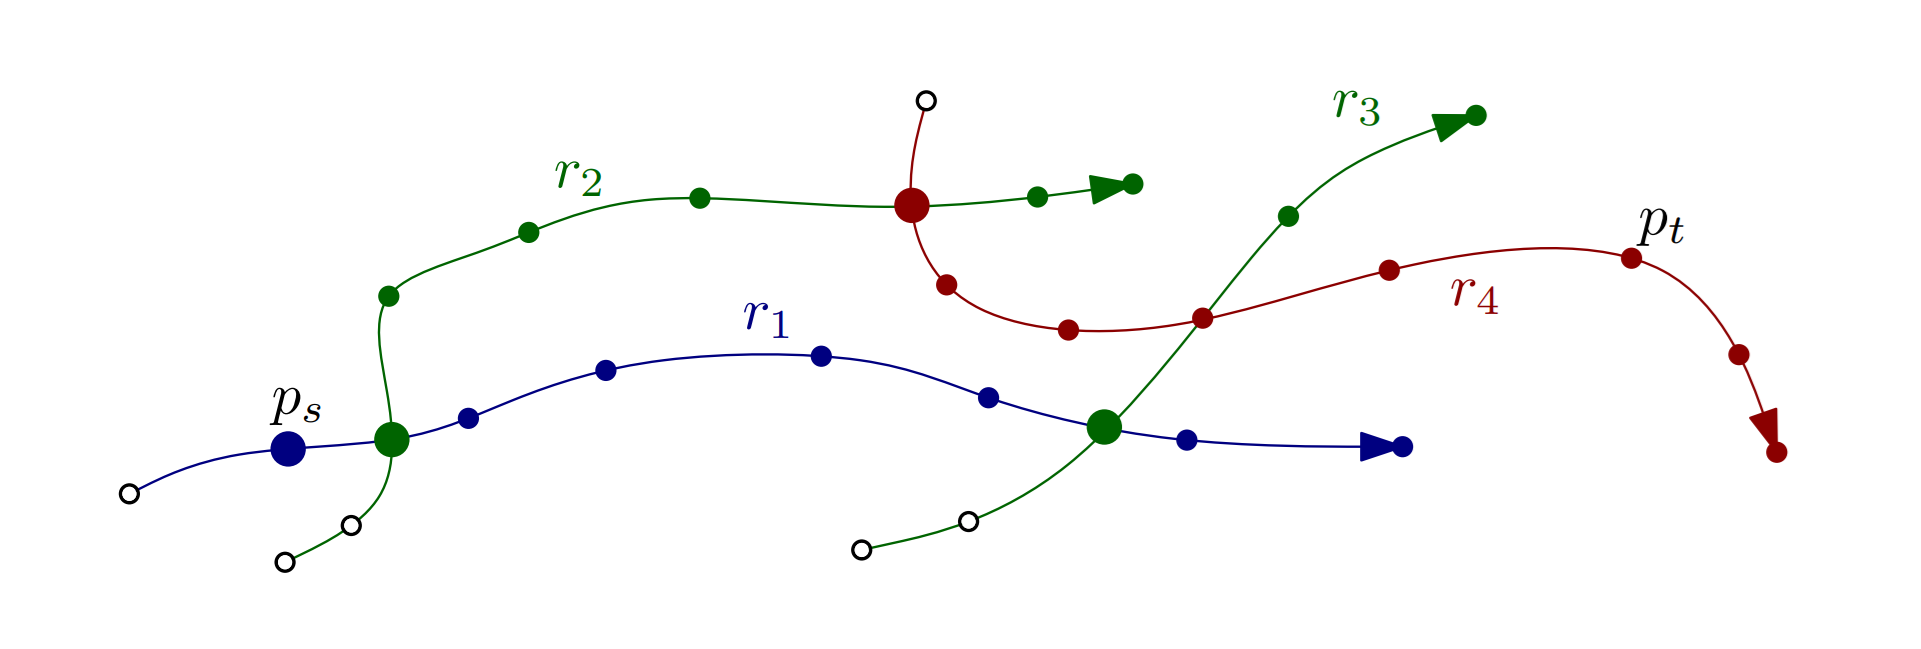
\includegraphics[width=\textwidth]{img/raptor_illustration.png}
    \caption[RAPTOR algorithm illustration]{Scanning routes for a query from p$_s$ to p$_t$. Route r$_1$ is first scanned in round 1, routes r$_2$ and r$_3$ in round 2, and finally, route r$_4$ in round 3. Scanning a route begins at the earliest marked stop (bold). Hollow stops are never visited. Source: \textcite{delling2015raptor}}
    \label{fig:gtfs_scheme}
\end{figure}


After this step is finished, it proceeds to the last step - traversing the transfers. This means that for every marked stop, it goes through all the neighboring stops to where a transfer can be performed and tries to relax their reach times. Once again, if their reach time was improved, it marks them.


This is repeated for a certain number of rounds. The design of the algorithm ensures, that after the n-th round, it has found the best reach time to every stop when using n or less public transit trips. In other words, after the first round, we get the best reach times at stops when only using a single direct trip from the source (and maybe a single transfer to the destination). In the second round, we add the option to transfer once to a different public transit trip and get all the best reach times with a maximum of 2 trips. Same as Dijkstra's algorithm, RAPTOR also finds the best times to all stops within the network, unless it is halted earlier. It can also simply be modified to reconstruct the best connections' path by storing not only the single best reach time, but an array of the best reach times in every round at every stop, together with an array of trips or transfers using which the stop was best reached in every round. Detailed information on the construction of the graph used by the algorithm, along with its pseudocode, can be found in \textcite{delling2015raptor}. 

In our application, we also want to include shared bikes in the search. Using this algorithm, this is actually very simple to do by inserting a new step between the trip traversals and transfer traversals, where we traverse all possible bike trips from every currently marked bike station and try to relax the reach time at the destination.

This algorithm has been shown to be faster than Dijkstra's algorithm and its modifications\cite{delling2015raptor}. It also has the useful feature of providing for every stop the best connections with every possible (and useful) number of trips. For example, if the destination stop can be reached with 0 transfers in 30 minutes, with 1 transfer in 25 minutes and with 2 transfers in 20 minutes, we can recover all of these options and provide them to the user as multiple alternatives. More information on the design of this algorithm and its variations (one of which, the rRAPTOR, our application uses for range searches) can be found in \textcite{delling2015raptor}.

\subsection{Calculating transfers}
\label{subsec:calculating_transfers}

Unfortunately, no data is available on what transfers are possible within Prague's public transit network and how long they take. Due to this, we will have to calculate the transfers ourselves. As we are already using a map router for shared bikes routing, we have the option of using this for walking transfers as well. However, the number of stops within the network is significantly higher than the number of bike stations and these computations would take an extreme amount of time. Additionally, we would also need to store this calculated distance data somewhere and the amount of space it would take up would be very large as well.

Another option is to use a constant global transfer time. This would obviously be very easy to implement, but there are also significant drawbacks to this approach. Mainly, we want our application to support transfers of a wide range of lengths (in particular, we support transfers of up to 750m of length, which turned out to be a great compromise between not having to process too many transfers and providing opportunities for as many time-improving transfers as possible). A constant transfer time could never account for both transfers that may be 0 or just a few meters long and transfers that are upwards of 500m long. Thus, we didn't go with this approach.

The approach we chose is to calculate the straight-line distance between every pair of stops and use this value to approximate the transfer's length and time. Obviously this value will almost never be exact, but it provides us with enough information to make an approximation of the actual length (by using these straight-line distances with a constant multiplier like 120\%).

When using the straight-line approach however, we face an issue in places where there are pairs of stops that are near each other, but it is not actually possible to transfer between them. An example of this would be stops on opposite sides of a river, railway track or a highway. To solve this issue without having to perform expensive map routing calculations, we prepared two simple files describing coordinate lines that may not be crossed by any transfer. First, we specify coordinate points in the \texttt{forbidden\_transfer\_points.csv} file and then describe lines between them in the \texttt{forbidden\_transfer\_points.csv} file, which cannot be crossed during a transfer. In Prague, most of these typically correspond to a river's path, a railway or a significant vertical drop. As our application is only targeted at Prague, there is no issue with managing these small files manually and adding new lines when necessary, as the number of such places is low, thanks to the city's street network being very dense and interconnected.

\subsection{Calculating bike routes}

As was already explained earlier, we will use a third-party library to implement bike routing. This is because for bike trips, which can be upwards of 4 kilometers long, the straight-line approach no longer gives us great approximations of the trips' length, as at that length, the actual shortest route's length may deviate significantly from the calculated straight-line approximation. Same as for the transfers, a constant global bike trip time makes no sense either. Due to all this, we will need to calculate the actual routes between the bike stations. 

We could theoretically use an external third-party API that provides this functionality, however these APIs are typically paid and are not effective for calculating such a large amount of trips. We could also implement a solution ourselves, however that would mean implementing a whole new application, the size of which would far exceed the scope of our project. Thus, we settled on using a library that was designed for this purpose.


\chapter{User documentation}

This chapter provides details on how to install the client application and how to use all of its features. It also explains how to use the server-side API, in case someone would want to build another client application, for example to support the iOS operating system as well.

\section{Client installation}

As we have not yet published the application on the official Play Store, it is necessary to first allow unknown app installation on the used Android device in order to install and use it. This permission needs to be granted to the browser application through which the user wishes to download the app. After this step is performed, the user only needs to visit the application's online repository\footnote{https://github.com/matejsubrt/PragO}, select the desired release of the app and download the \texttt{prago-<version>.apk}\footnote{https://github.com/matejsubrt/PragO/releases/tag/0.1.0} file. After it is downloaded, simply tap the file in the downloads section and follow the installation guide. 

Please note that after first downloading the app, it first needs to download the current data on stops within the network in order to provide stop name suggestions. As this step uses a significant amount of data, it will only be performed when the device is connected to the internet using Wi-Fi. This step may also take a longer time depending on your internet download speed. Thus, we recommend first downloading and launching the app while connected to a Wi-Fi network. Subsequent updates of this data will be performed automatically in the background when connected using Wi-Fi connections and thus do not require any special care.

\section{Client usage}
\label{subsec:usage}

In this section, we will go over the different parts of the application, their user interface and the features they provide.

\subsection{Search screen}

The search screen is the first screen that the user will be presented with after launching the application. It contains the main input fields and most of the toggles and sliders necessary to meet the functional requirements. Only a few settings that are not expected to be changed frequently have been moved to the settings screen.

As you can see in \cref{fig:search_screen}, the search screen contains the inputs for the source and stop names. A click on these leads the user to the stop selection screens, where they can actually select the stop they want. There is also a toggle to flip the direction of the search.

Under the stop name inputs is the row with time settings. First, it contains an icon indicating whether the search is currently set to consider the set time to be the earliest possible departure, or latest possible arrival time. Next to this, the currently set time is displayed. When clicked, this takes the user to the time select screen, where they can select both the time and the departure/arrival setting. Finally, there is a "Now" button at the end that resets the time settings to an earliest departure at the current time.

Under the time row, there is a simple toggle for using shared bikes within the search. 

Finally, there is the section with extended settings. These contain some of the search customization options we decided to provide with our application. The section is minimized by default, but clicking on it reveals its content, as you can see in \cref{fig:extended_settings}. Within this section, the user can set the transfer buffer (corresponds to the \cref{req:transfer_buffer} requirement), the maximum transfer length (\cref{req:max_transfer_distance}) and the balance between shortest time and least transfers (i.e. comfort preference, \cref{req:comfort_balance}). Furthermore, if "Use Shared Bikes" is set to true, this section also contains the slider for setting a bike trip buffer (\cref{req:bike_trip_buffer}) and a toggle to limit the maximum bike trip duration to 15 minutes (\cref{req:bikes_max_15}).

Apart from the source and destination points and the time settings, all other entered values are preserved in between app launches to prevent having to modify them every time the app is being used.

\begin{figure}[h!]
    \centering
    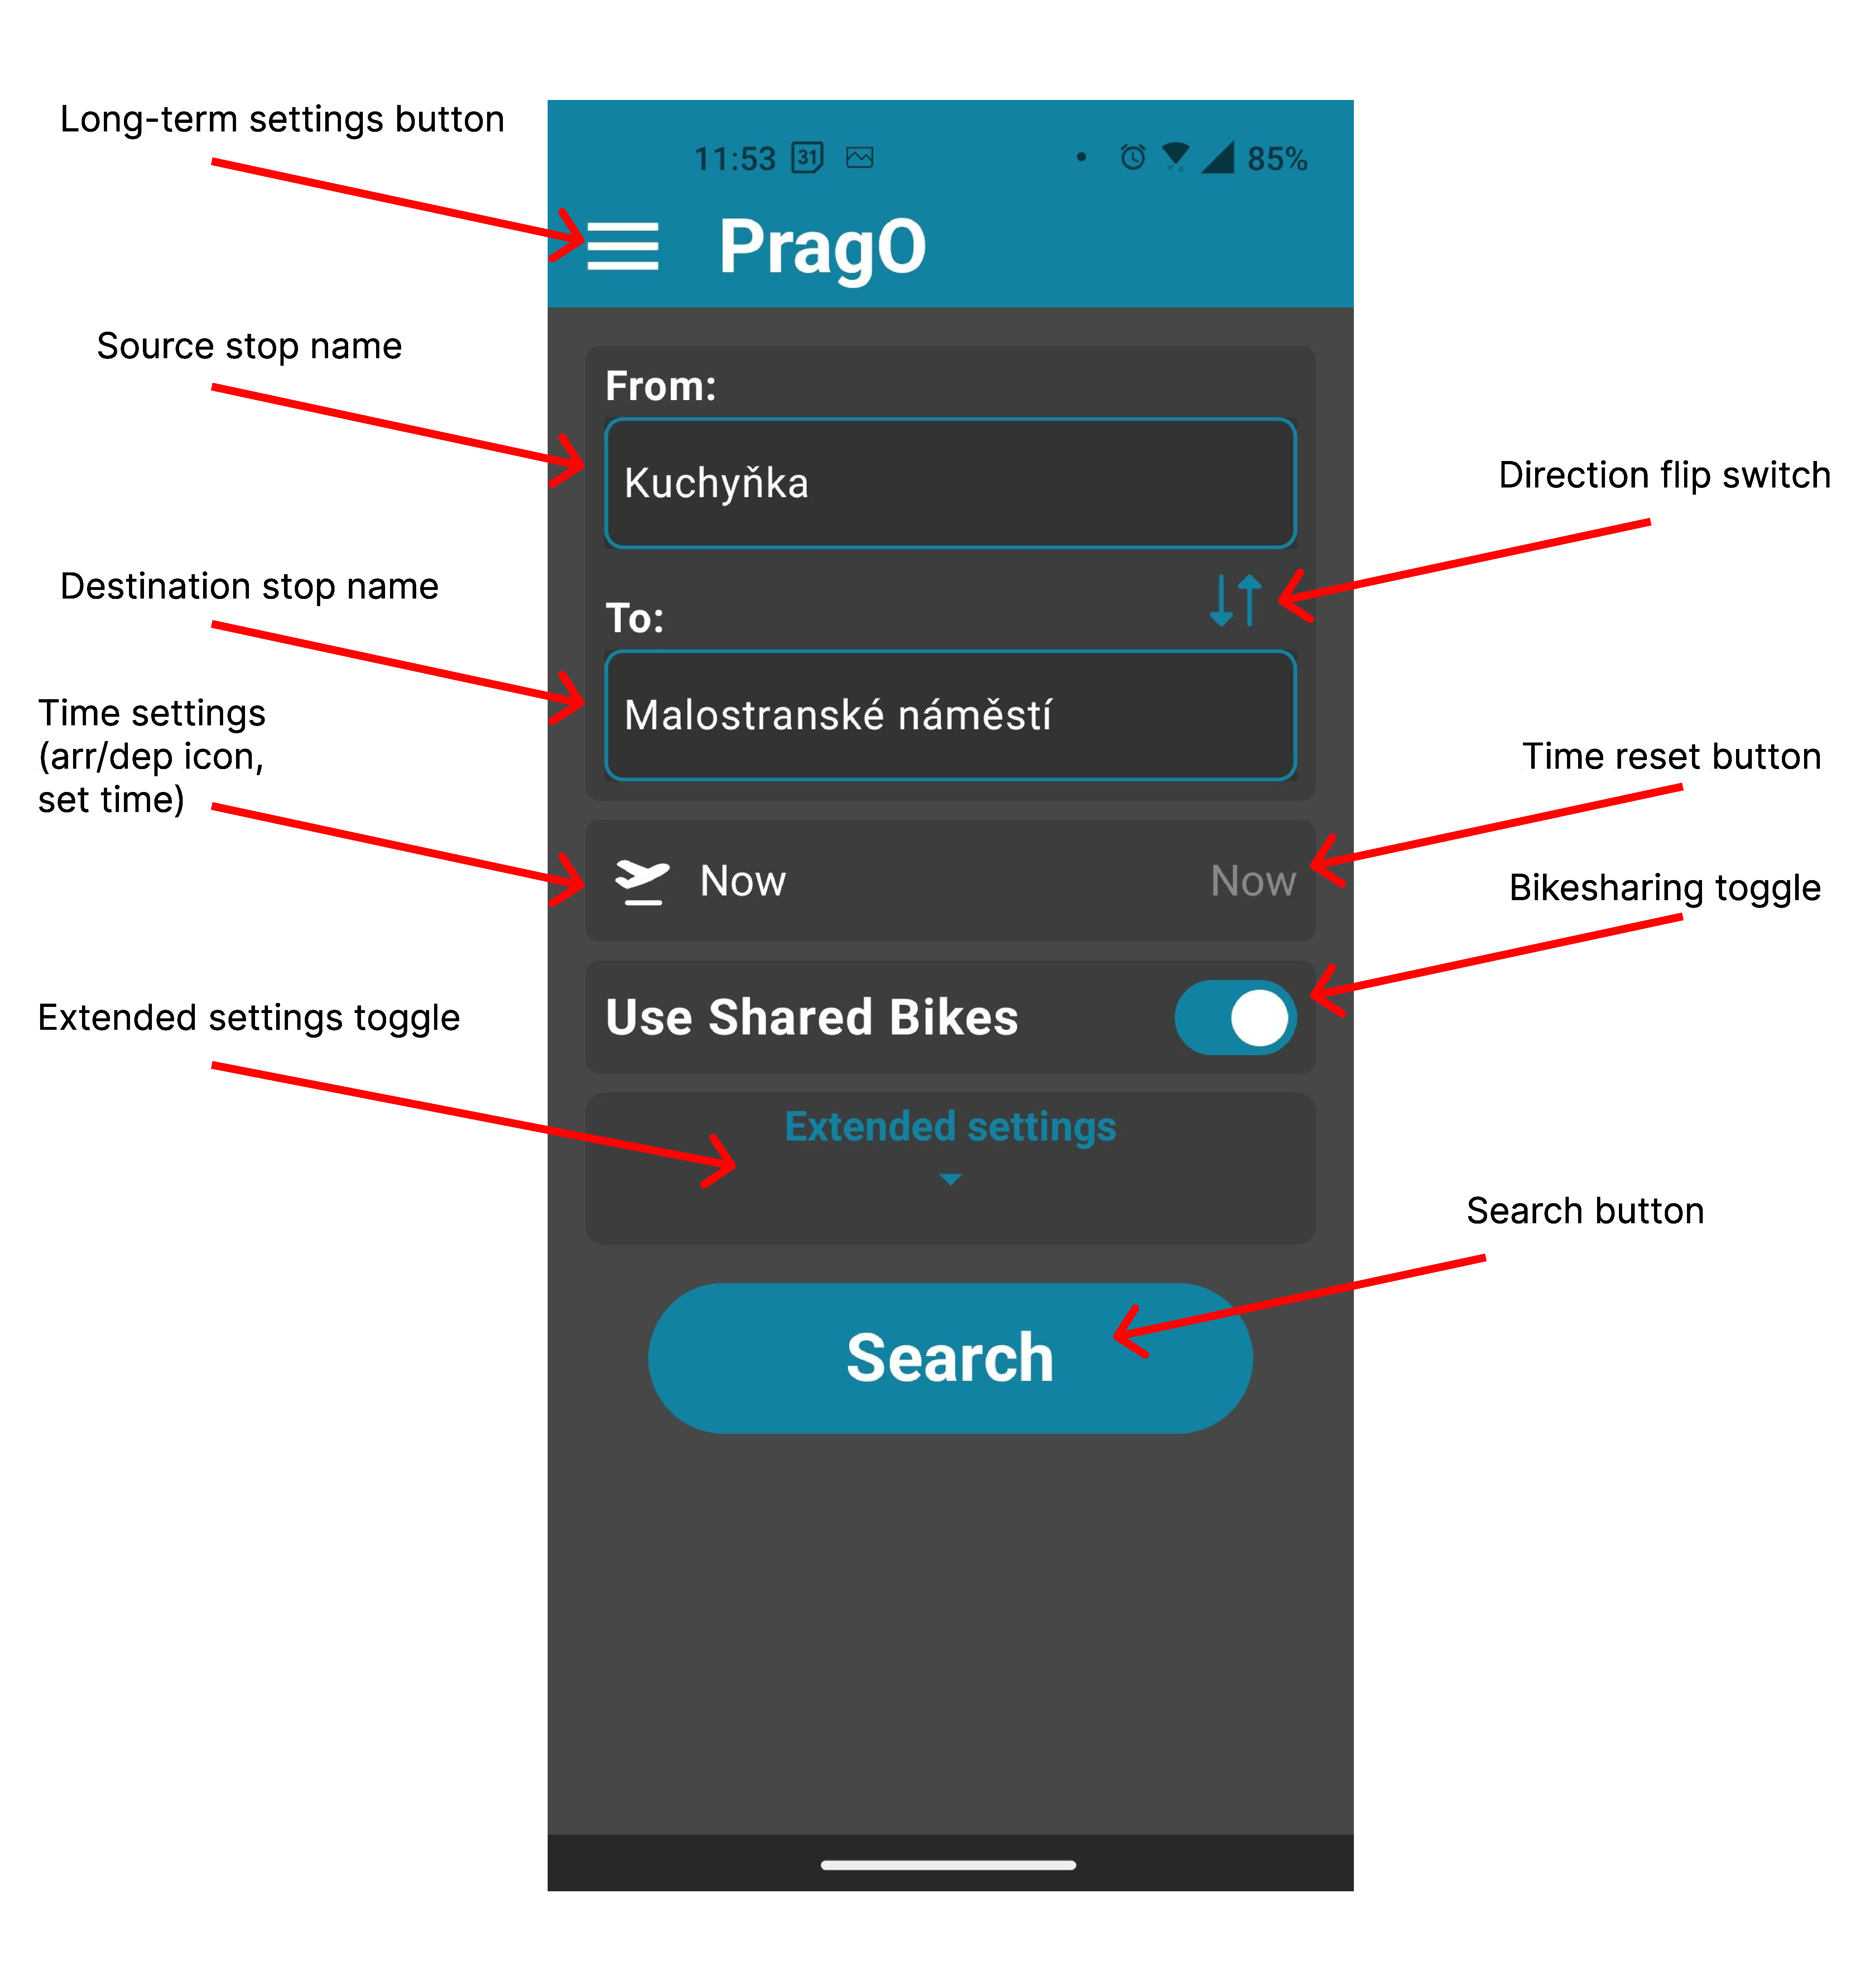
\includegraphics[width=\textwidth]{img/ui_descriptions/search_screen.pdf}
    \caption{Search screen overview}
    \label{fig:search_screen}
\end{figure}

\begin{figure}[h!]
    \centering
    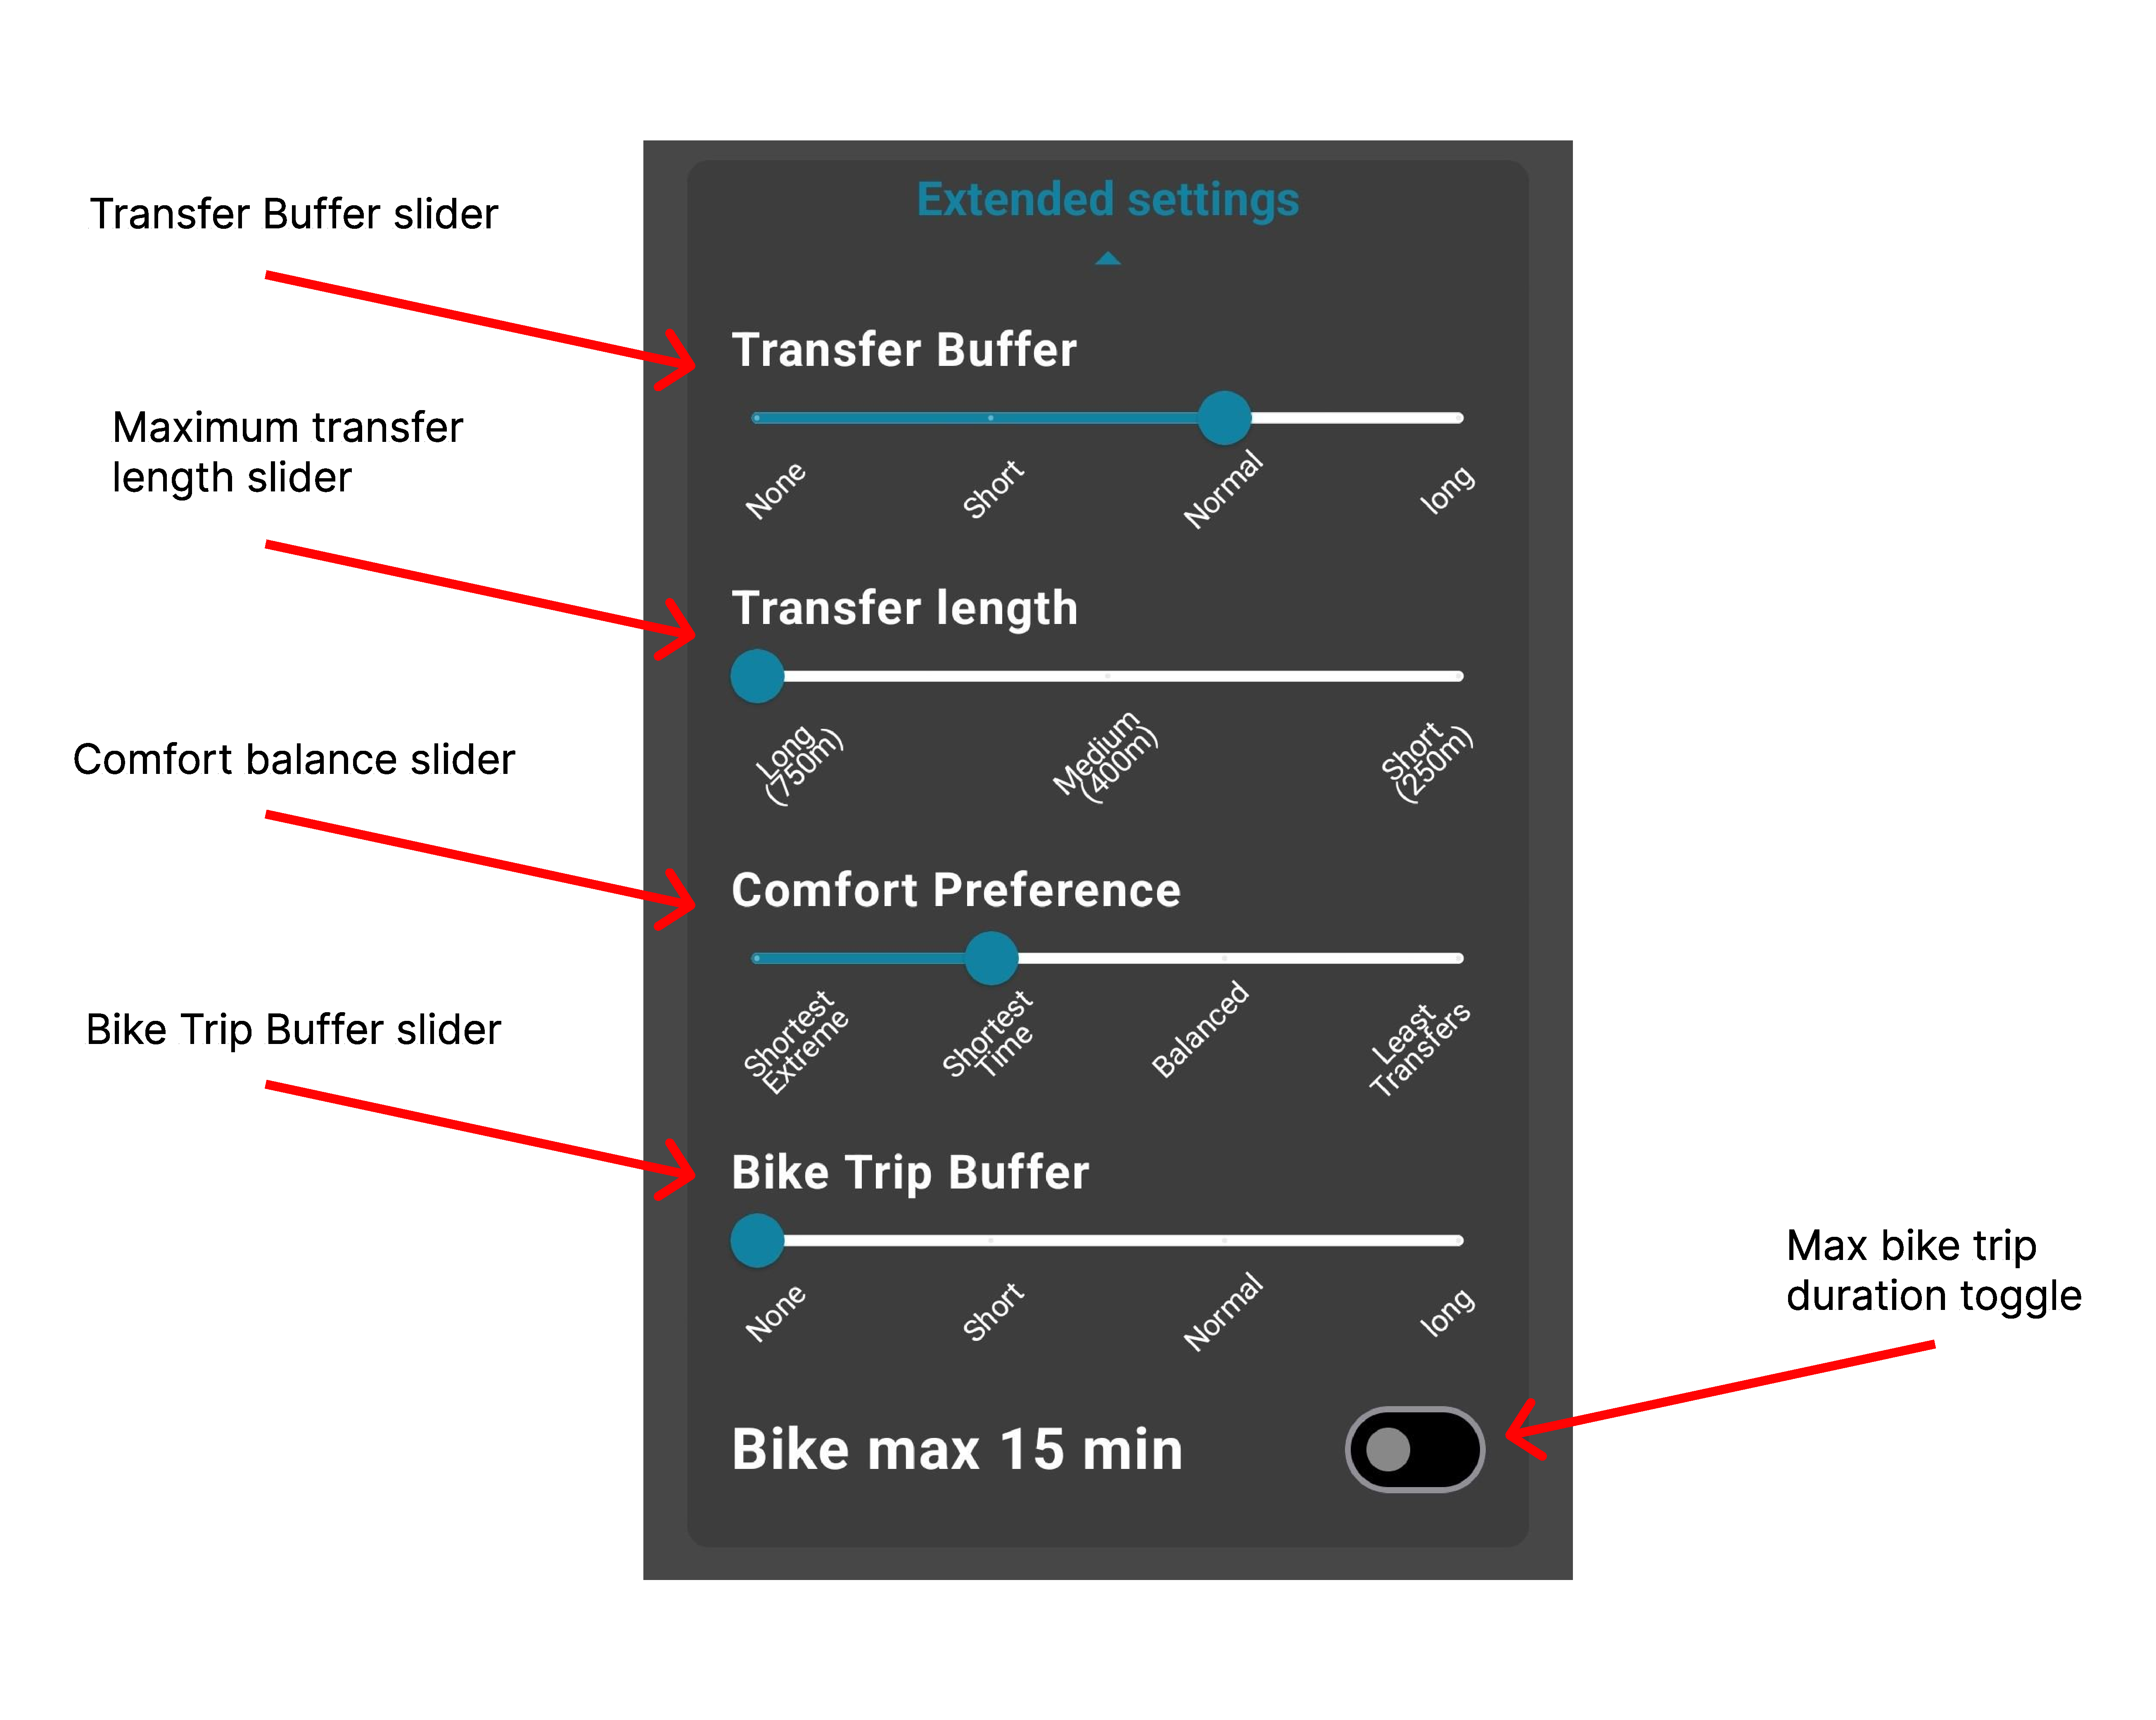
\includegraphics[width=\textwidth]{img/ui_descriptions/extended_settings.pdf}
    \caption{Extended settings section}
    \label{fig:extended_settings}
\end{figure}

\newpage

\subsection{Stop select screen}

This screen (see \cref{fig:stop_select}) will appear when the user clicks on any of the 2 stop selection fields on the search screen. Apart from being able to return back to the search screen via the return button at the top, the user can select the source or destination stops here by typing out their names. The application supports improved searching, which means that for multiple-word stop names, the user can only type the beginnings of each word (i.e. \textit{"mal nam"} for \textit{"Malostranské náměstí"}), and the application will provide the corresponding suggestions (\cref{req:stop_name_suggestions}). Upon clicking on any suggestion, the application saves this preference and returns the user back to the search screen. There is also a delete button that deletes the entered text if the user wants to start from the beginning.

Additionally, when setting the source, the user also has the opportunity to select the "My location" suggestion, which will start the search using the user's current coordinate location instead of using a stop name (\cref{req:src_by_coords}). Note that for this to work, the user must allow the application to use their location in the popup that will appear.

\begin{figure}[h!]
    \centering
    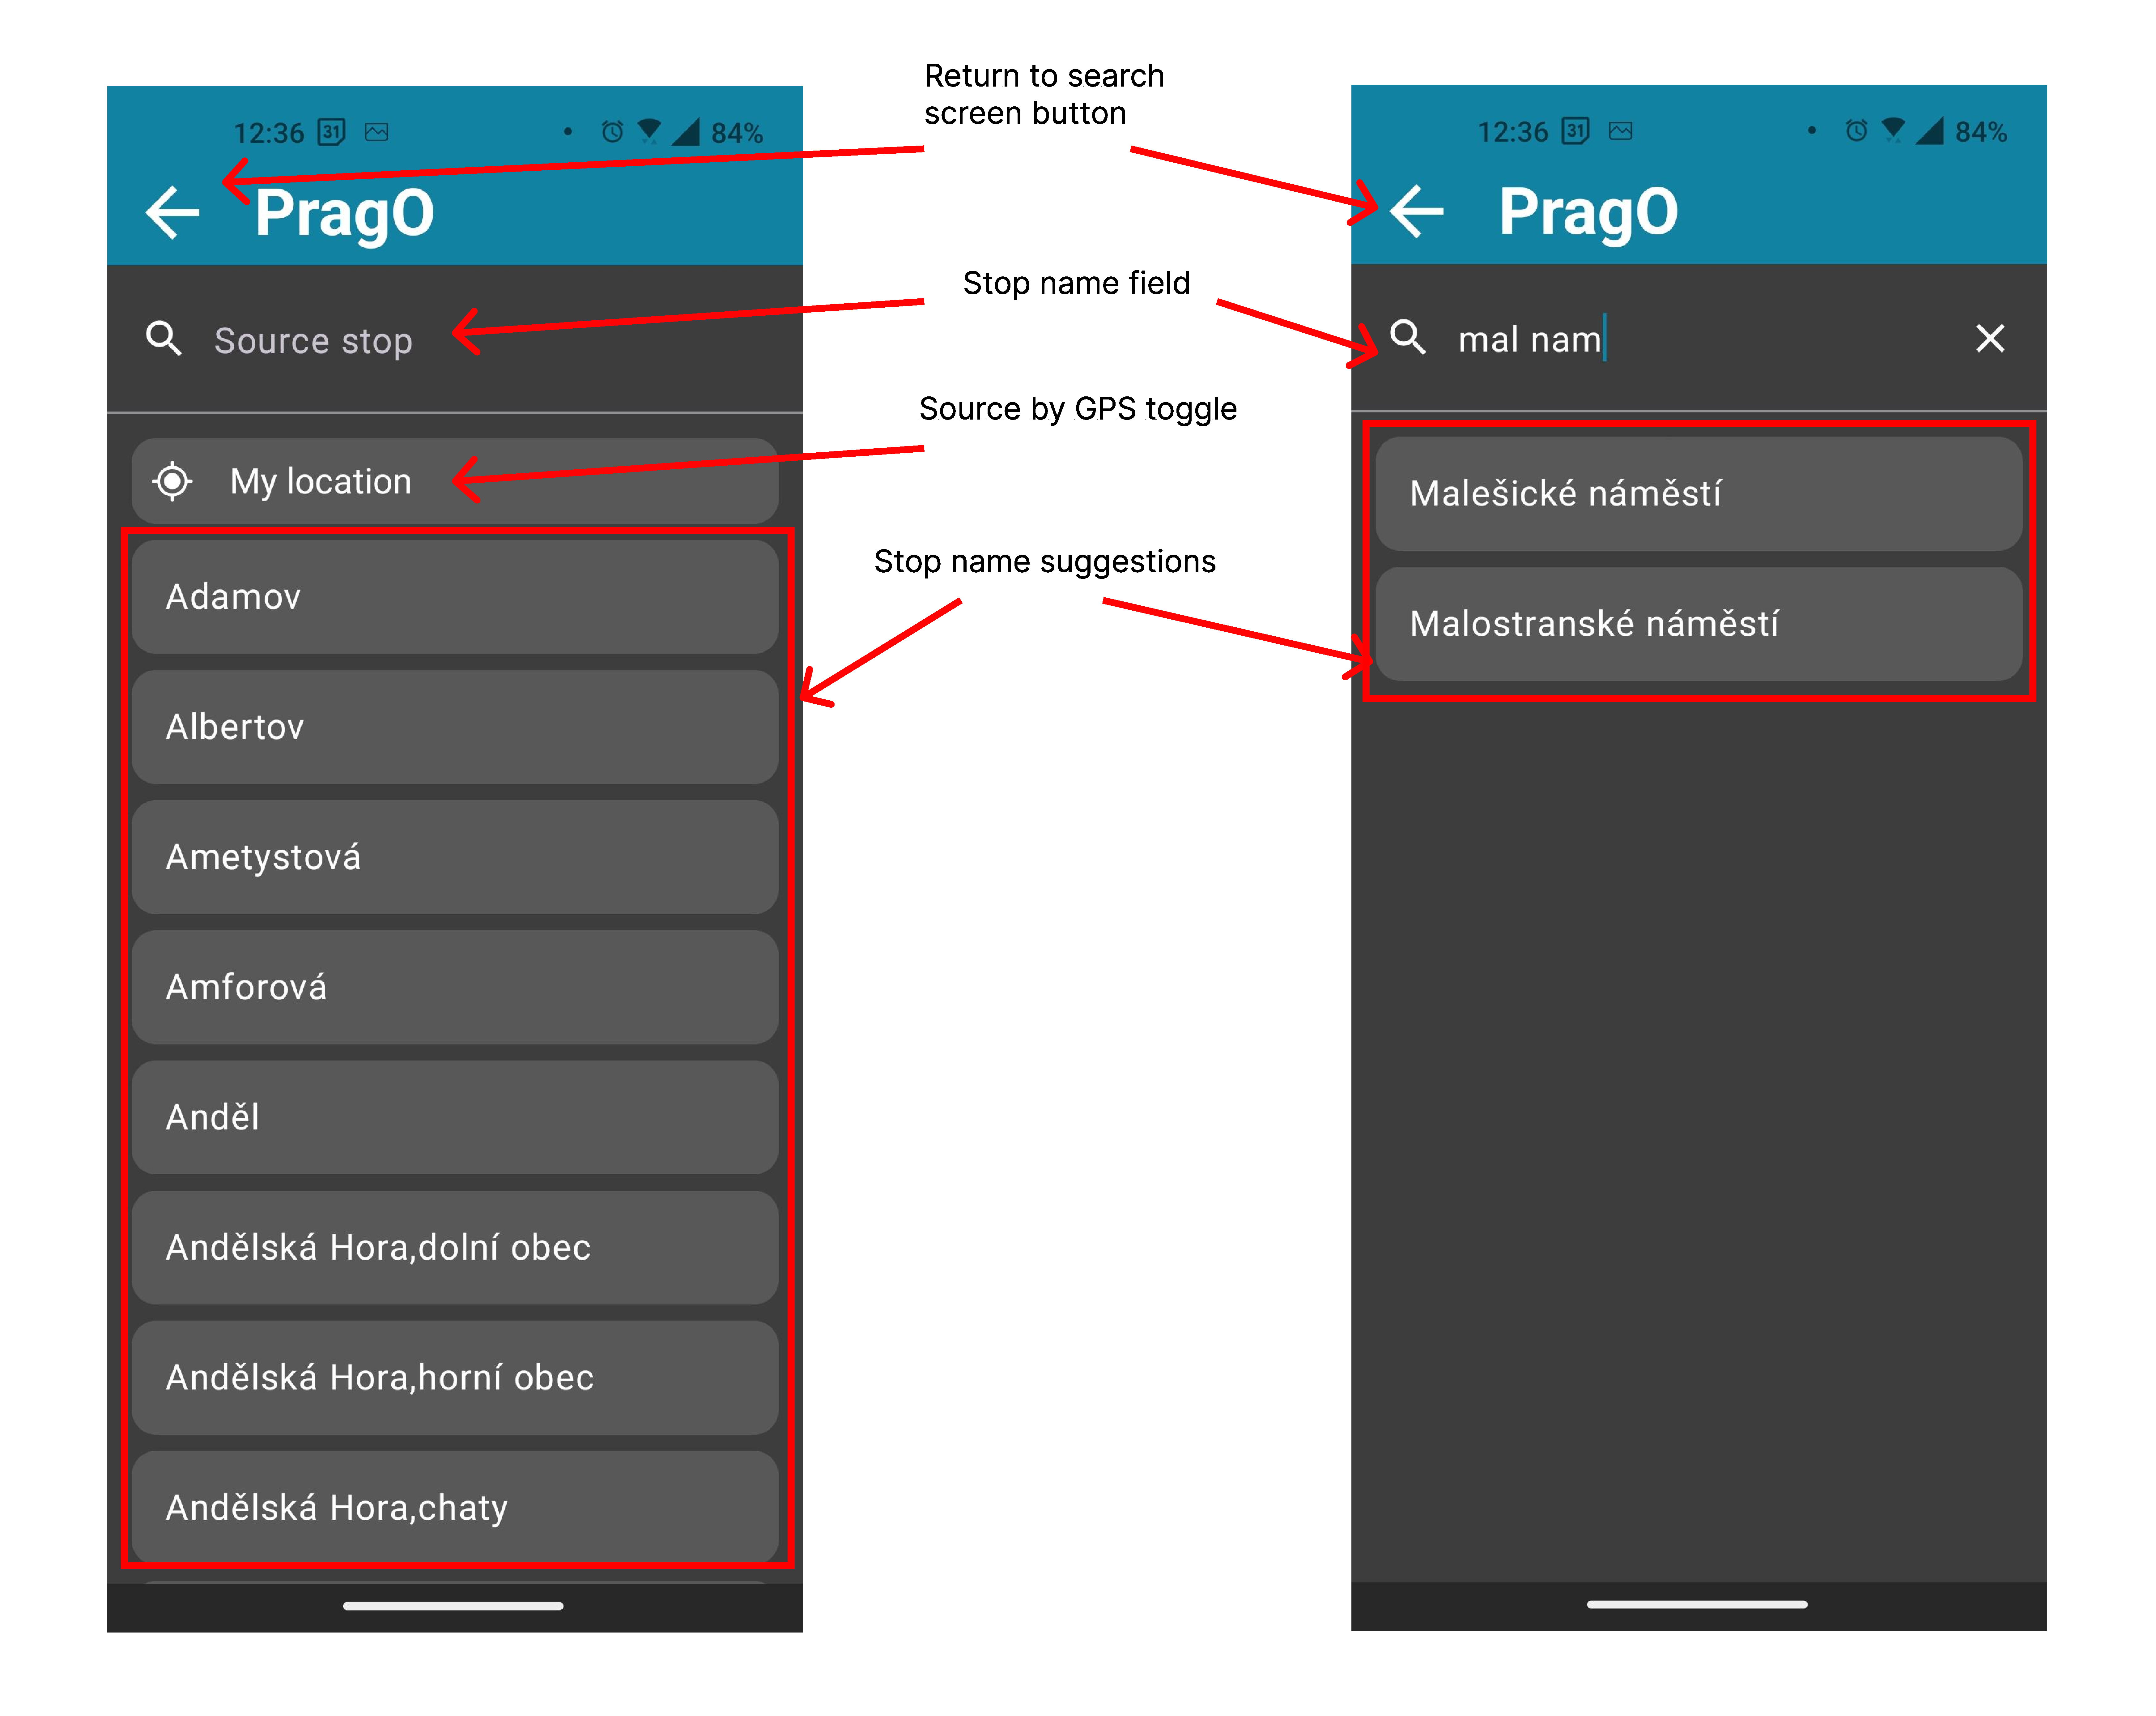
\includegraphics[width=\textwidth]{img/ui_descriptions/stop_search_screen.pdf}
    \caption{Stop select screen}
    \label{fig:stop_select}
\end{figure}

\newpage


\subsection{Time select screen}

On this screen (see \cref{fig:time_select}), the user can adjust all the time settings. They can change the date via the date setting wheel, the time via the time setting wheel and the meaning of the selected time, i.e. whether it sets the earliest departure or latest arrival boundary (\cref{req:arr_dep_time}). Upon clicking the "Done" button, the user is taken back to the search screen.

\begin{figure}[h!]
    \centering
    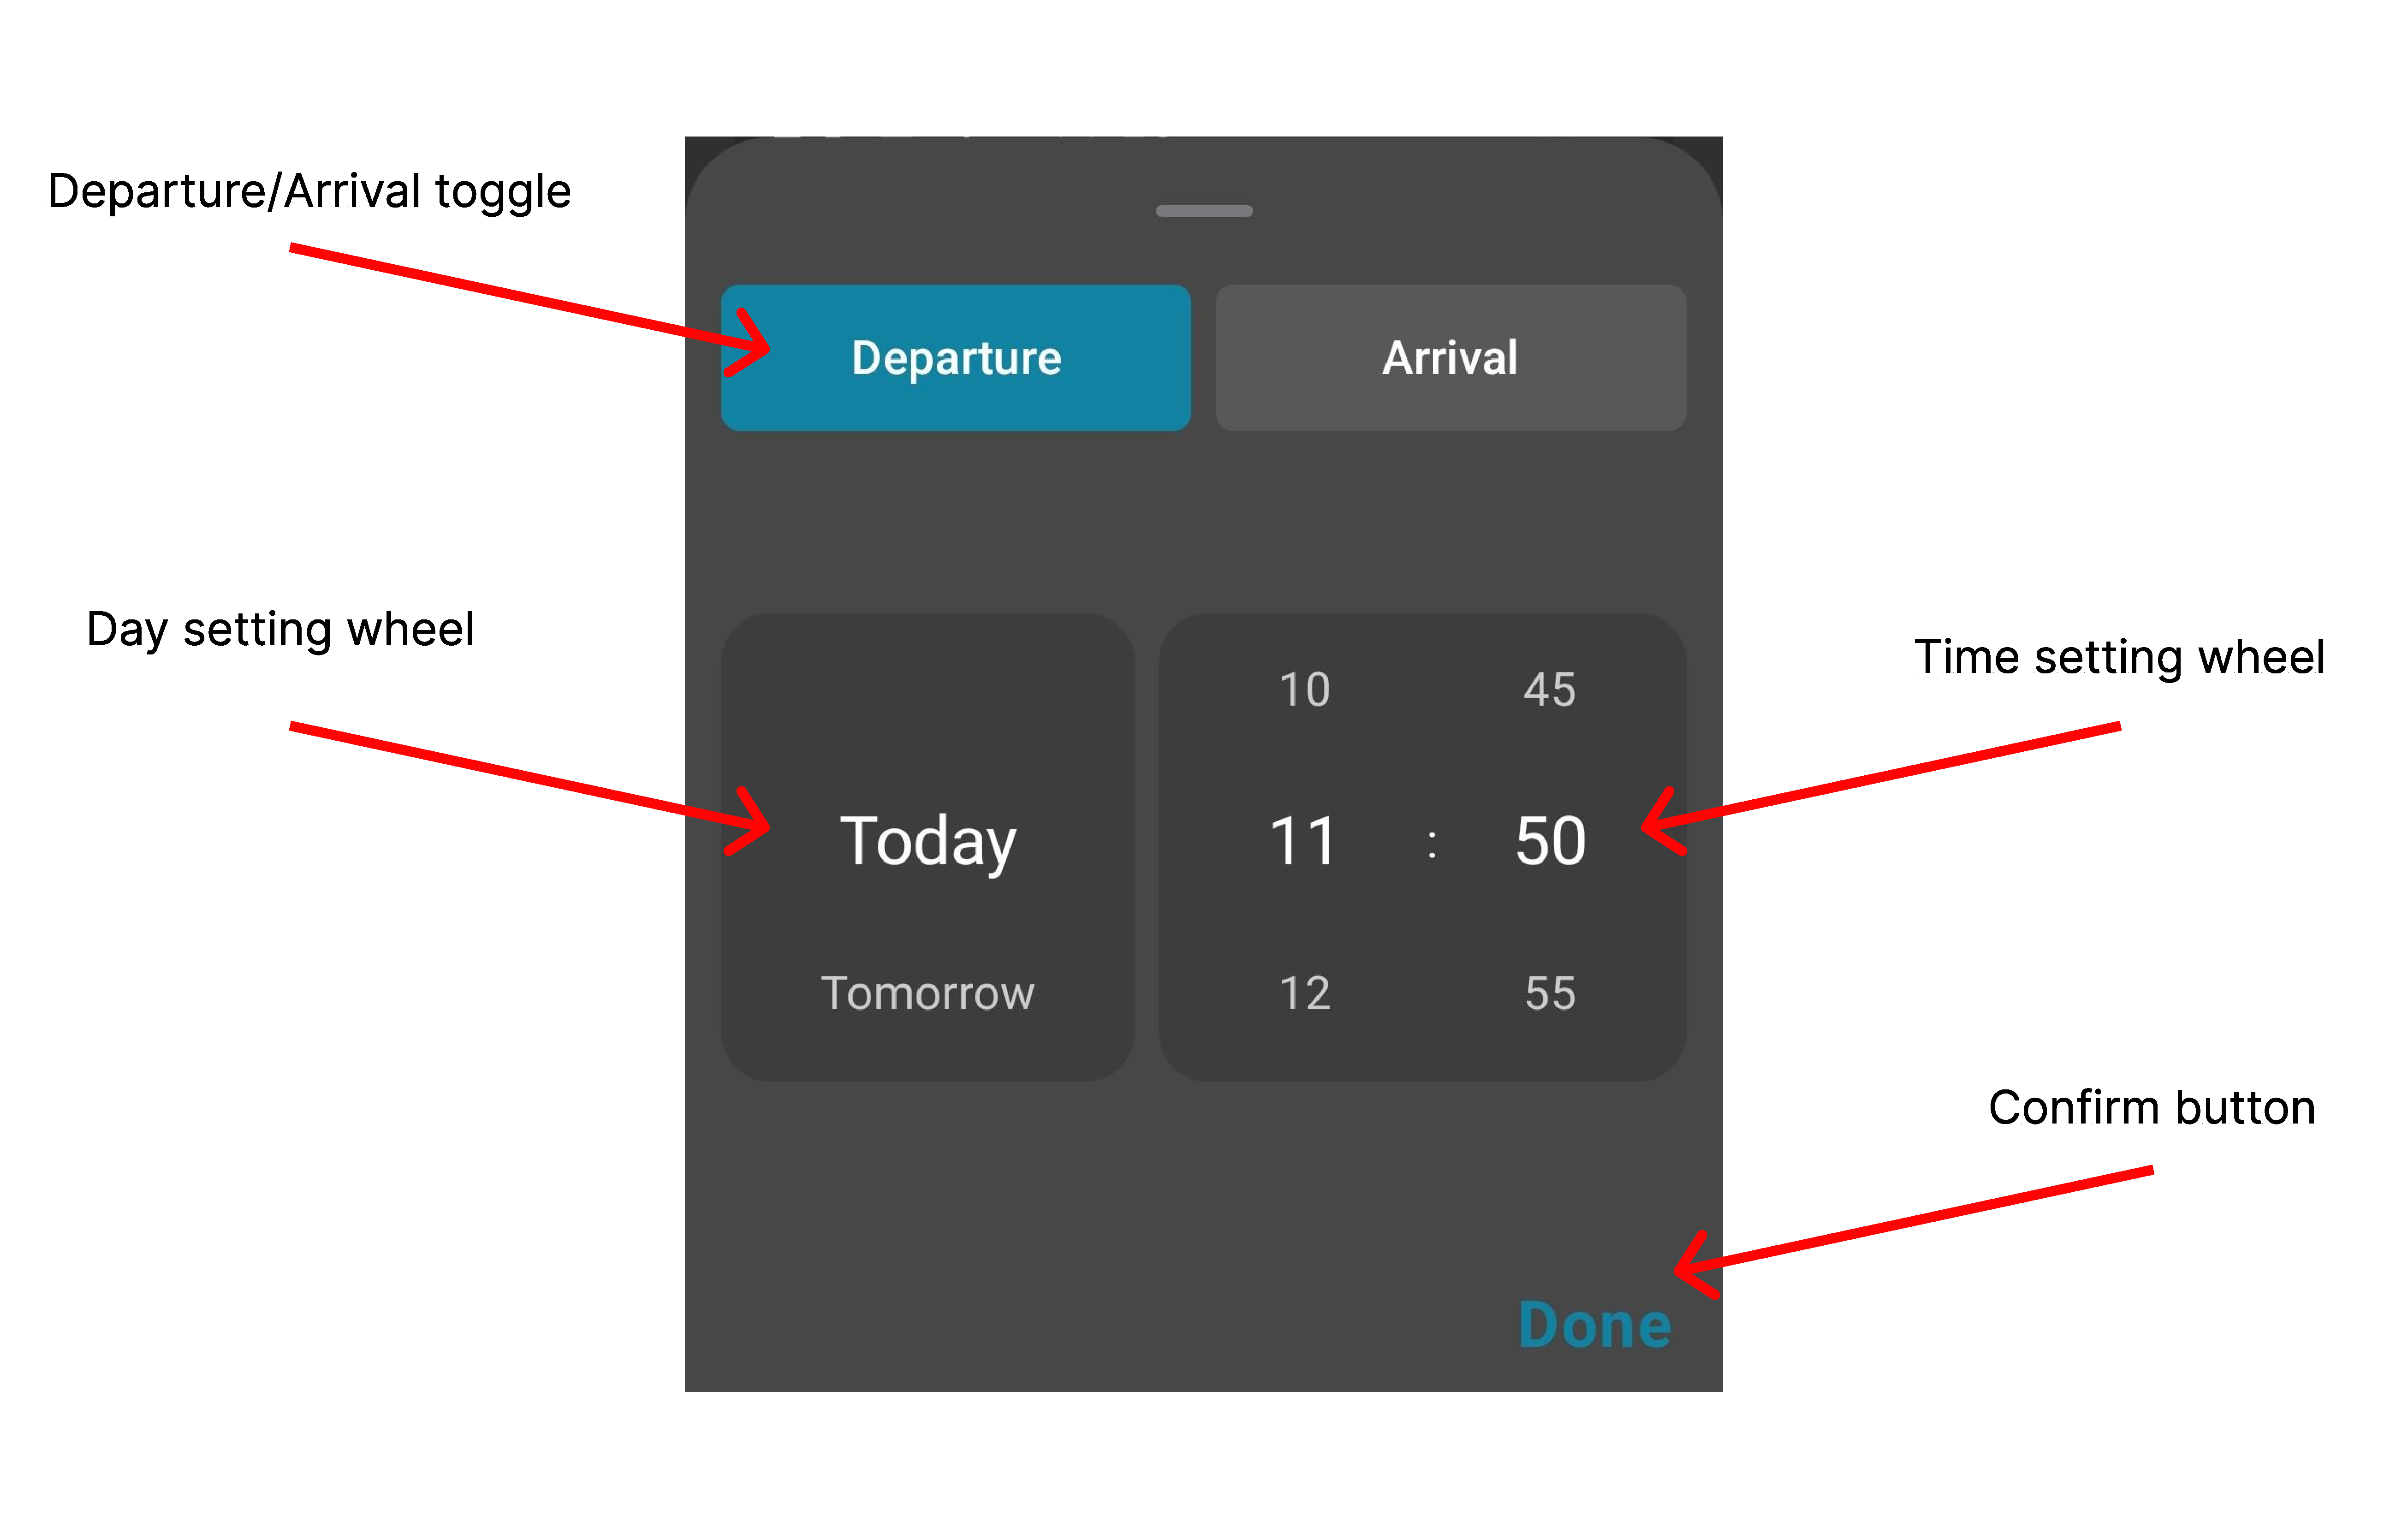
\includegraphics[width=\textwidth]{img/ui_descriptions/time_settings.pdf}
    \caption{Time select screen}
    \label{fig:time_select}
\end{figure}

\newpage

\subsection{Settings screen}

This screen provides access to all the settings that typically do not change very often and thus do not need to be included on the main search screen. As you can see in \cref{fig:settings_screen}, these include setting the walking pace (\cref{req:walking_pace}), cycling pace (\cref{req:cycling_pace}) and the shared bike lock and unlock times (\cref{req:lock_unlock_time}). By clicking the "Save and return" button, the user saves the values and returns to the search page.


\begin{figure}[h!]
    \centering
    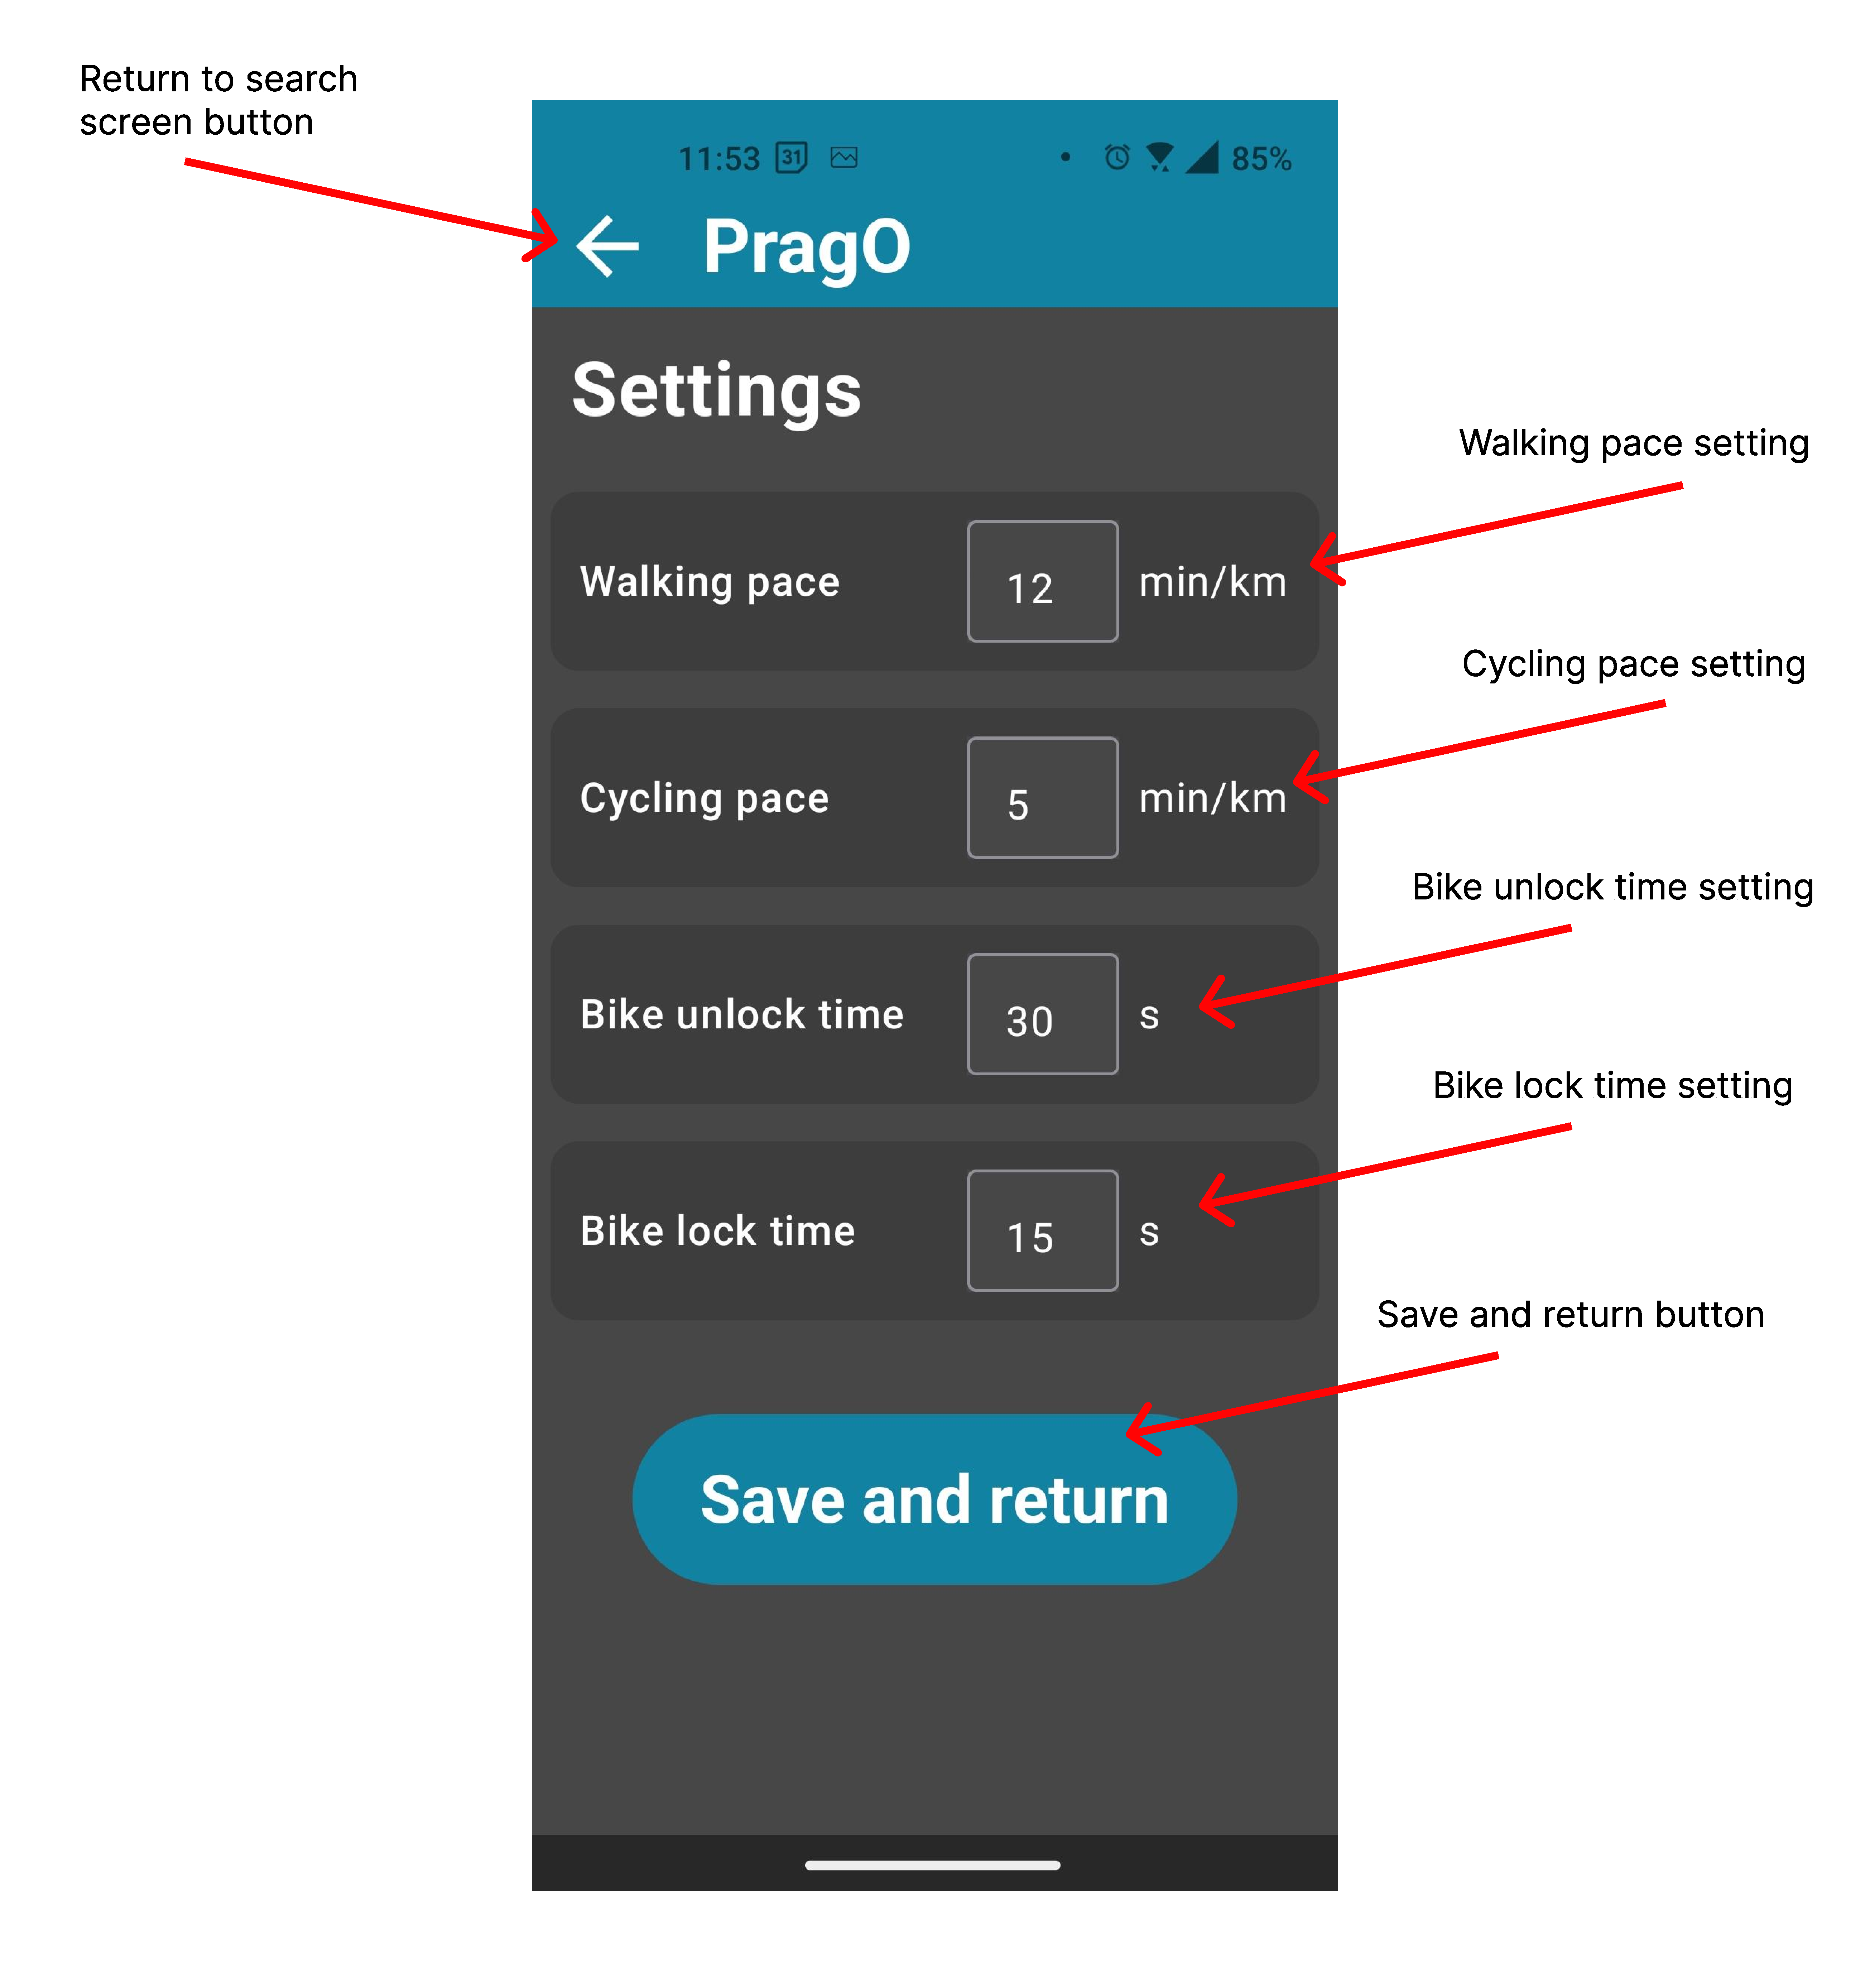
\includegraphics[width=\textwidth]{img/ui_descriptions/settings_screen.pdf}
    \caption{Settings screen}
    \label{fig:settings_screen}
\end{figure}

\newpage


\subsection{Results screen}

This is where the results of the search get displayed. According to requirement \cref{req:multiple_results}, our app does not just search for a single connection, but rather searches for multiple best connections across a time range. In particular, the app first searches for the best connection according to the given parameters. Then, if the user scrolls further down the page, it loads further later connections. If the user wants to view earlier connections, they can pull down while on top of the page, which will expand the results into the past.

Every individual result is displayed in the form of a single connection card. As you can see in \cref{fig:results_screen}, this card contains all the necessary information about all the segments of the connection. At the top, there is a countdown until the connection leaves and the total duration of the connection (\cref{req:countdown}). Furthermore, the countdown has 3 variations - in cases, where the connection immediately begins by boarding a trip at the source stop, only a countdown until boarding the trip is displayed (see "Time until first departure" in \cref{fig:results_screen}. In cases where the connection only consists of transfers and bike trips, there is no time limitation as to when the connection may be performed. Thus, such connection are marked as "Anytime" (see "Departure possible anytime" in \cref{fig:bike_results}). Finally, in cases where the connection begins with a transfer and later down the line continues with a trip, two countdowns are displayed - one showing the time left until the first trip leaves and a second one showing the time left until the user should start the initial transfer (see "Time until initial transfer start" in \cref{fig:results_screen}). If the first trip has not yet departed, but the time at which the user was supposed to start walking to make the connection has already elapsed, the first trip countdown is highlighted to remind the user of this situation (see "Time left until first trip departure" in \cref{fig:bike_results}).

Every segment within the connection then has a separate section within the result card. For a trip, the line name, together with the boarding and disembarking stops and exact times (\cref{req:exact_times}) and the current delay (\cref{req:delays}) of the trip are displayed. For a transfer, the distance and expected duration are shown. Finally, for a bike trip, the application displays its source and destination bike stations' names, the distance and expected duration of the trip, and the current number of free bikes available at the source station (\cref{req:bike_count}) (see \cref{fig:bike_results}).

The user can also swipe left or right on any of the displayed public transit trips to reveal its earlier/later alternatives (\cref{req:trip_alternatives}). It is also possible to click on any of the displayed bike trips, which (when connected to the internet) will take the user to the Mapy.cz application and display the route they are supposed to take. Note that the length of this displayed route might vary slightly from the distance specified in our app, as we use a different routing engine and map data for our searches.

\begin{figure}[h!]
    \centering
    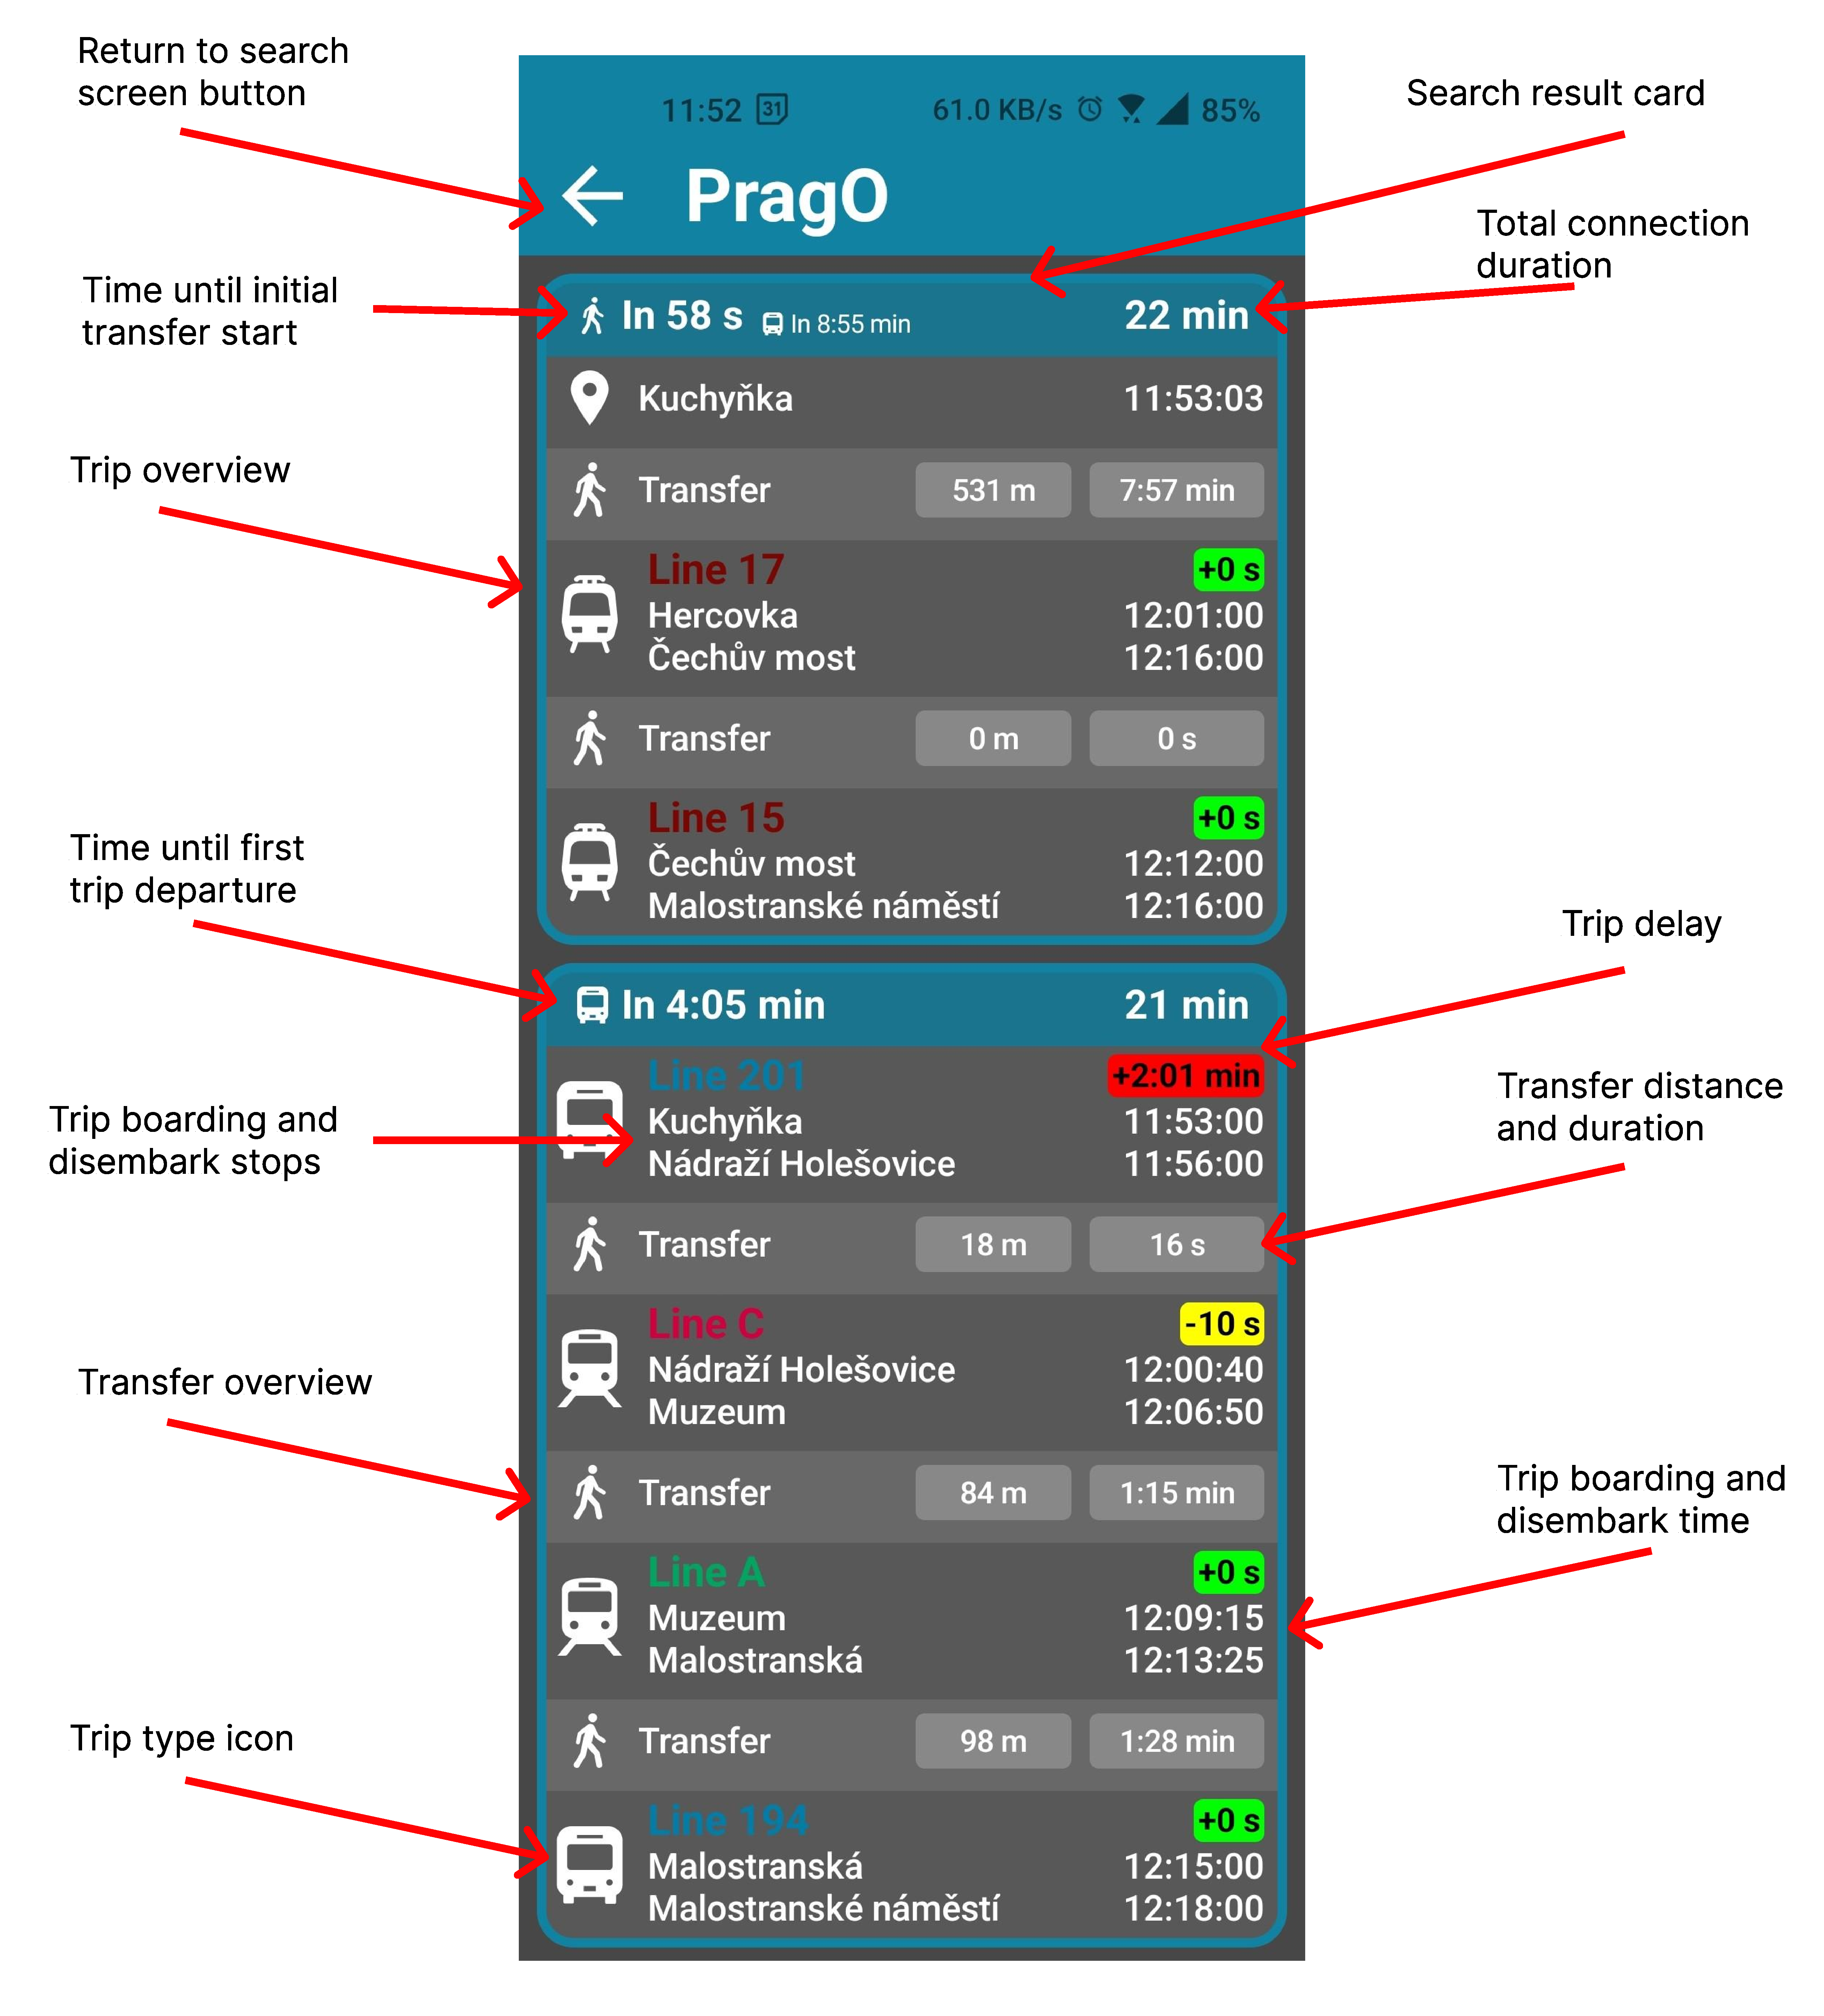
\includegraphics[width=\textwidth]{img/ui_descriptions/result_screen.pdf}
    \caption{Results screen}
    \label{fig:results_screen}
\end{figure}

\begin{figure}[h!]
    \centering
    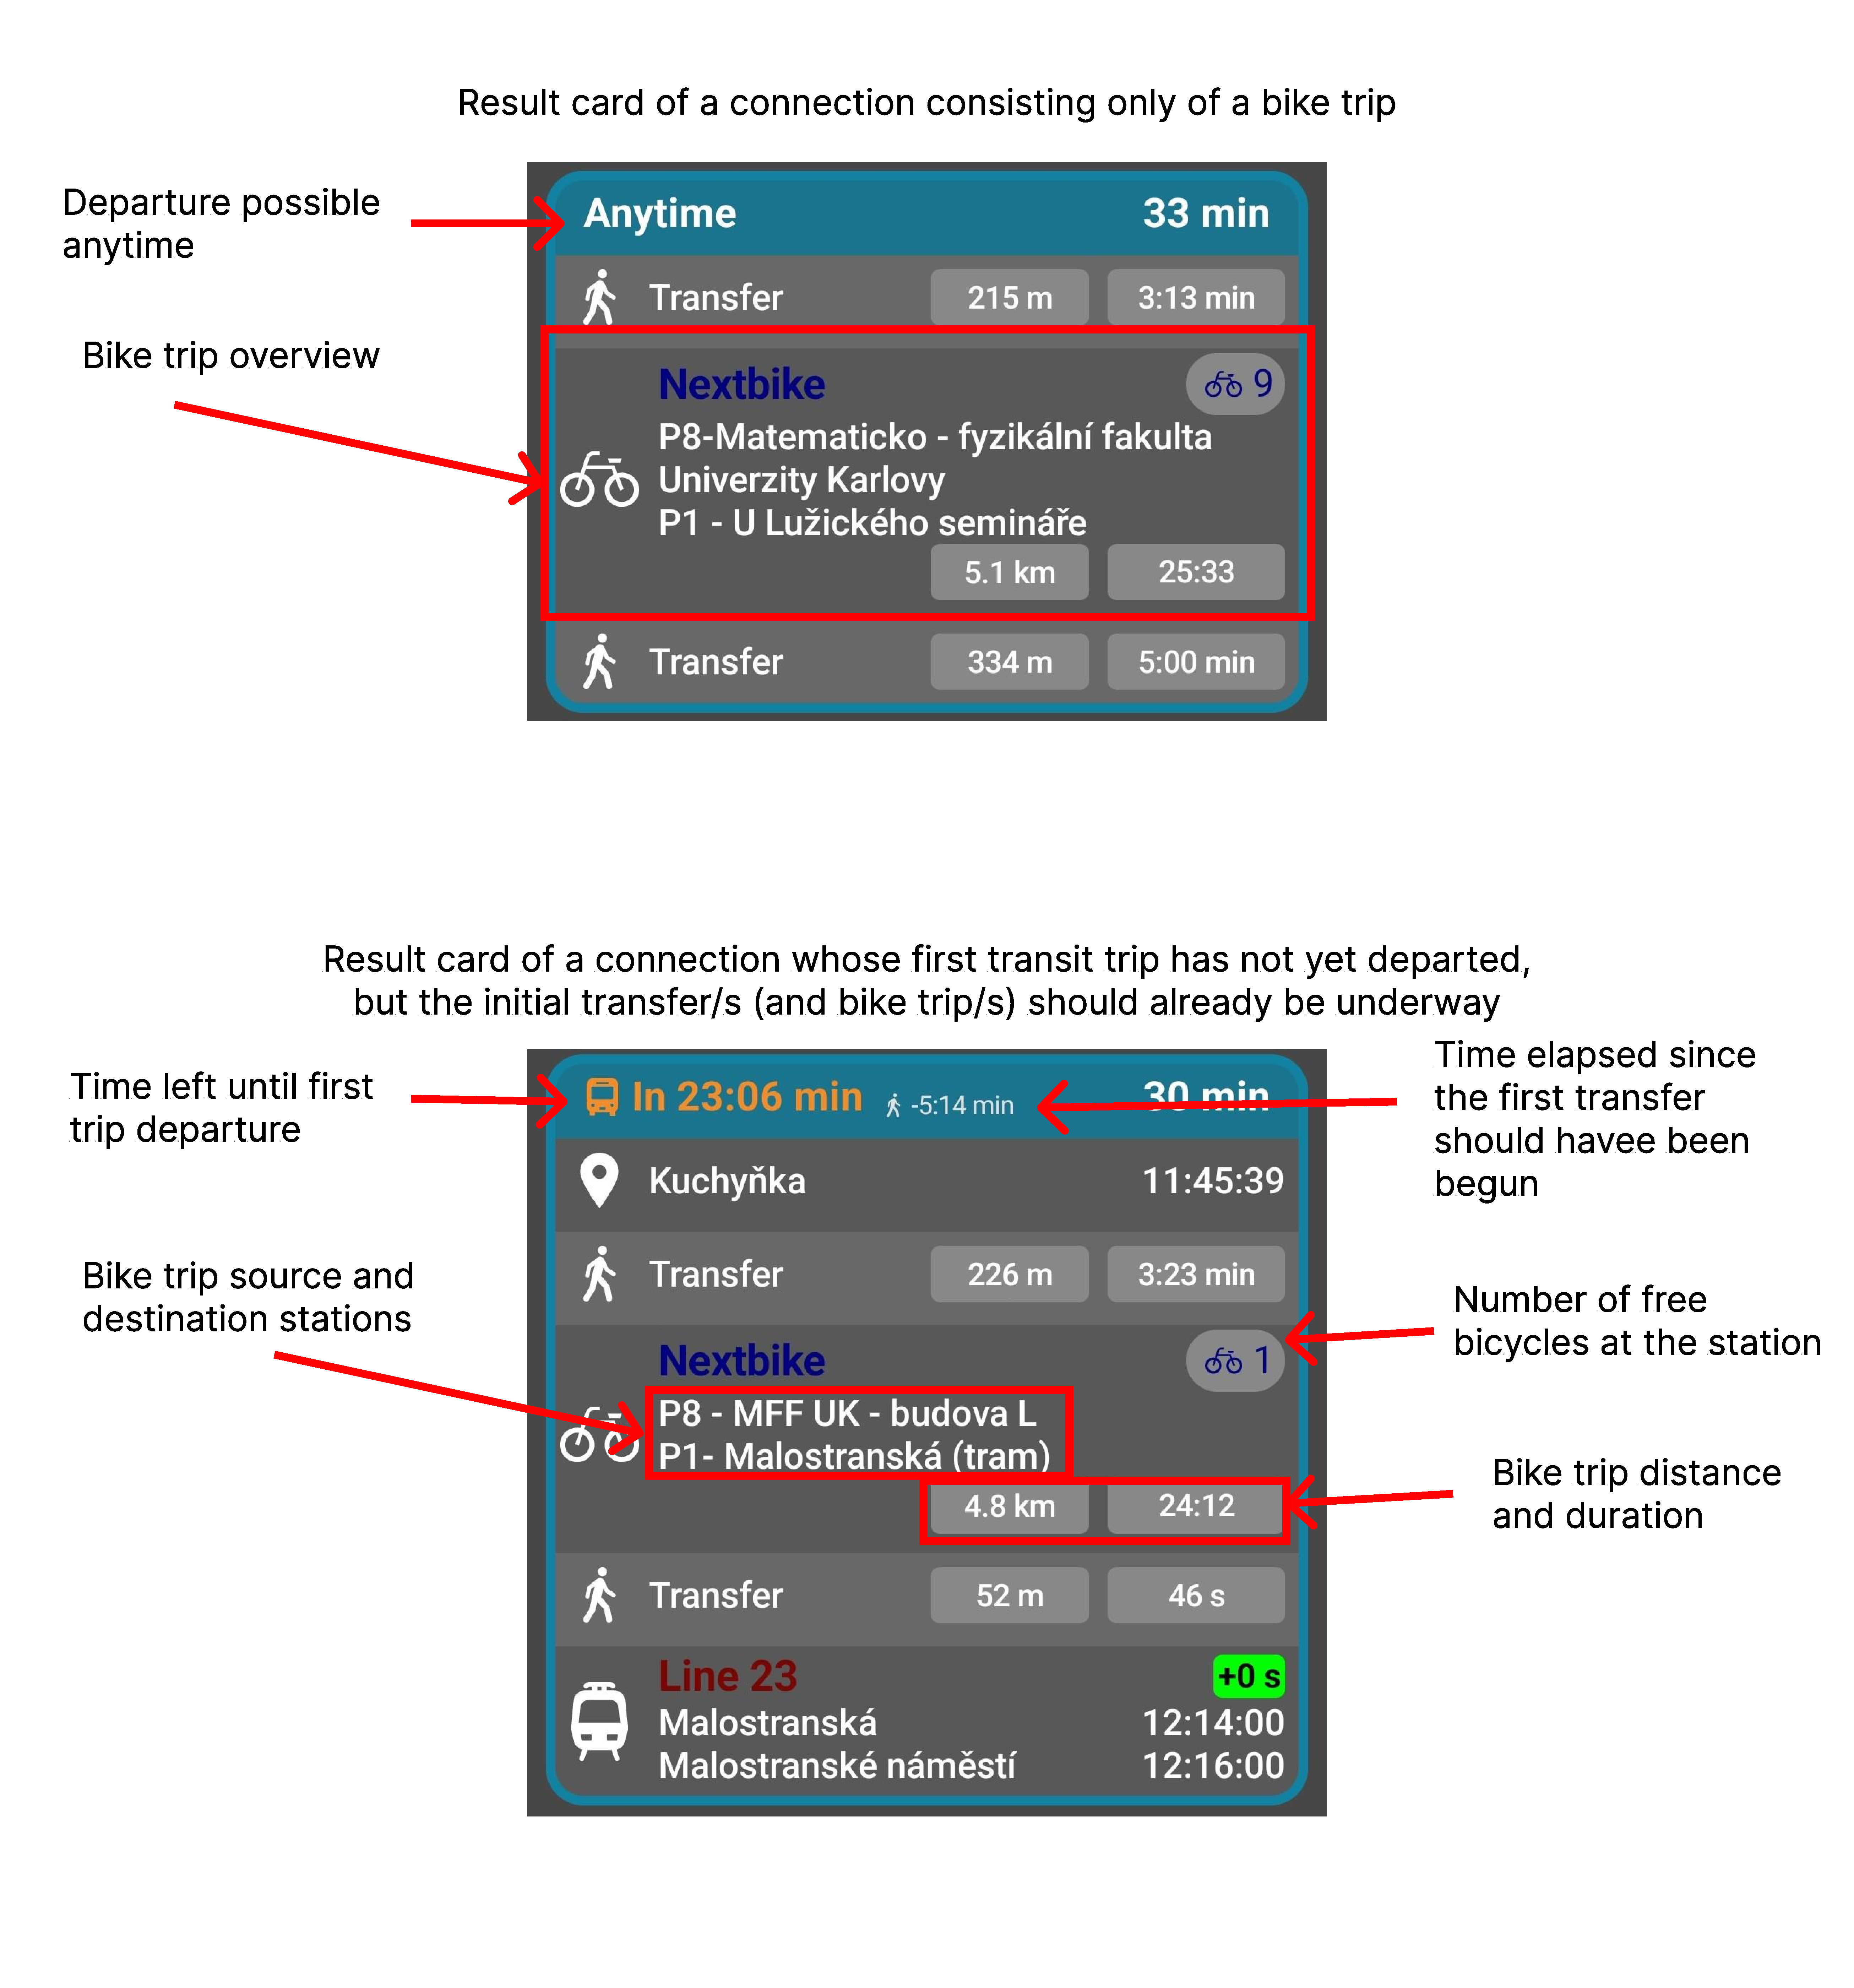
\includegraphics[width=\textwidth]{img/ui_descriptions/bike_results.pdf}
    \caption{Bike result cards}
    \label{fig:bike_results}
\end{figure}


\section{API usage}

Apart from using the provided client application, it is also possible to use the back-end API directly. There are 3 distinct POST endpoints - a connection search endpoint, a trip alternatives endpoint and a delay updating endpoint. Let's go over them and explain their purpose. Note that when running the server-side application in the WebAPI (and not WebAPI-light) configuration, the exact schemas of the requests and responses, as well as other information about the API, can be found on the address \texttt{<BASE-URL>/swagger/index.html}, so we will not be showing them here.

\subsubsection{Connection search endpoint}
\label{subsec:connection_endpoint}

The connection search endpoint at the address \texttt{<BASE-URL>/connection} is the main endpoint for connection searching. It takes a connection request object containing all the search parameters including the source and target locations, the specified time and the settings for the search. It returns a list of the first relevant connections for the search parameters. This endpoint is also used for search expanding - in case the client already has some results and wants to request later ones, it can send the same request with the time set to the departure of the last existing result and the \texttt{byEarliestDeparture} parameter set to \texttt{true}. Analogically, when expanding to the past, time is set to the arrival time of the earliest existing connection and \texttt{byEarliestDeparture} to \texttt{false}.

This endpoint may respond with the codes \texttt{200: OK} if the connection was successfully performed, \texttt{404: Not Found} in case no connection was found for the parameters and \texttt{400: Bad Request} in case any of the provided parameters or setting values were invalid. In that case, the response will contain a message with the reason for the failure.

\subsubsection{Trip alternatives endpoint}

This endpoint exists at the address \texttt{<BASE-URL>/alternative-trips} and serves the purpose of finding alternative direct trips. The client needs to provide the ids of 2 stops between which direct trips run and the id of the trip for which it wants to find the alternatives, a time and a parameter specifying whether to find earlier or later alternatives. The API will then respond with a list of alternative direct trips. Once again, the possible response codes are \texttt{200: OK} if found correctly, \texttt{400: Bad Request} when some of the parameters were invalid or \texttt{404: Not Found} when the alternative trips could not be found.

\subsubsection{Delay updating endpoint}

\xxx{Hasnt this changed???}

This endpoint at the address \texttt{<BASE-URL>/update-delays} has the same input and output parameter. It takes a list of existing results, goes through all trip alternatives of all trip segments of all the results and updates all their delay data. Then it returns these newly updates results. This endpoint only returns the code \texttt{200: OK}, as it discards results which it cannot process.
\chapter{Developer documentation}

This chapter is focused on the actual implementation of the different parts of our application. It describes the structure of the code and the decisions made when writing it. It also explains the steps necessary to build and launch the application on a new server. Although the main focus is on the main server part of the application, it also describes the basic functioning of the Android client.

\section{Server application}

As already mentioned above, we decided to build the back-end side of our application in the C\# programming language, and thus it needs the .NET environment to run. In this section, we will first go over the application's directory structure and the installation process. Then we will go through the server's implementation and the code structure.

\subsection{Directory structure}

At the top level, there are two main directories - the \texttt{src} directory contains all the code and the \texttt{docs} directory contains the generated programmer documentation. Here, you can find information on all the classes and interfaces within the project. Within the \texttt{src} directory, you will find the following items:

\begin{itemize}
    \item \xxx{ConnectionSearchTests} is a directory containing all the tests for the code.
    \item The \textbf{\texttt{RAPTOR-Router}} directory contains the main part of the application. Here, you will find all of the routing functionality.
    \item The \textbf{\texttt{WebAPI}} and \textbf{\texttt{WebAPI-light}} directories contain the implementation of the API. They use the \texttt{RAPTOR-Router} project to find the resulting connections and return these results. Their code is essentially identical and they provide the exact same functionality and API endpoints. The difference is that the light version uses a more stripped-out version of the .NET API to consume less system memory. We implemented this version to be able to run the application in strongly memory-constrained environments. In case your system has larger amounts of memory available, we recommend using the standard version, as it also provides automatically generated Swagger API documentation.
    \item The \textbf{\texttt{data}} directory contains all the necessary data that the application uses to run and provide routing.
    \item The \textbf{\texttt{config.json}} is a file that the program uses to find locations of necessary files and URLs of used APIs. It contains default locations for all files, however you may change these if necessary.
    \item The \textbf{\texttt{init.sh}} is an initialization script for the application. More information on this is presented in the followings section.
\end{itemize}

\subsection{Installation and launch}

To install and successfully run the server application, you will need to perform the following steps:

\begin{enumerate}
    \item First, you will need to ensure that the .NET runtime is installed on your machine. Our application requires .NET 7.0 or newer. For more information on this step, see Microsoft's official .NET installation guide\footnote{https://learn.microsoft.com/en-us/dotnet/core/install/}.
    \item After ensuring the .NET Runtime is installed:
    \begin{enumerate}
        \item If running the application on linux, you can use the provided \texttt{src/init.sh} initialization script. It ensures everything is prepared for the launch. As most of the data is provided as part of the application's repository, this mainly includes downloading the OSM map file, which is too large to be included with the application. You can provide the following options to the script:
        \begin{enumerate}
            \item \texttt{--osmPath <PATH>} specifies the directory into which to download the OSM file. By default, this is set to \texttt{src/data/osm\_routing}. Please note that when changing the location, it will be necessary to change the path in the \texttt{src/config.json} file.
            \item \texttt{-l/--launch} ensures that the script immediately launches the application after preparing the necessary data.
            \item \texttt{-n/--nohup} ensures that if \texttt{-l/--launch} is set, the application is launched as a service running in the background. Otherwise, the application is launched normally within the console.
        \end{enumerate}
        If you wish to only launch the application later, you can choose the version to run (i.e. WebAPI or WebAPI-light) and run \texttt{dotnet run -c Release} in the corresponding directory.
        \item Else, you will need to perform the steps manually. This includes:
        \begin{enumerate}
            \item Downloading the Open Street Maps map file, which will be used for bike trip routing. This can be downloaded from the OSM website\footnote{https://download.geofabrik.de/europe/czech-republic.html}. We recommend putting it into the \texttt{src/data/osm\_routing} directory, which is the default location where the program will look for the file.
            \item If it was installed into a different location, it will be necessary to adjust the \texttt{src/config.json} file accordingly.
            \item The application can be launched from either the \texttt{WebAPI} or \texttt{WebAPI-light} directory by running the command \texttt{dotnet run -c Release}.
        \end{enumerate}
    \end{enumerate}
\end{enumerate}



\subsection{API implementation}

As mentioned above, the \texttt{WebAPI} and \texttt{WebAPI-light} projects are essentially the same, except the light version is intended to run in memory-constrained environments and does not provide Swagger API documentation. The implementation of the API is very simple. In C\#, there are 2 main options as to how to implement an API - a controller-based and a minimal API approach. As our API is very small and simple with only 3 simple POST endpoints, we decided to use the minimal API approach to minimize unnecessary code complexity.

As explained earlier, there are 3 endpoints (\texttt{/connection}, \texttt{/alternative-trips} and \texttt{/update-delays}). Each of these takes its parameters and calls its \texttt{Handle} function using them. The \texttt{Handle} functions only perform basic data checks before calling the routing methods from the \texttt{RAPTOR-Router} part of the project, which we will describe in detail in the next section. After these functions return their results, the \texttt{Handle} functions check these results for errors and issue a HTTP response accordingly.

\subsection{RAPTOR-Router implementation}

This is the main and largest part of the application. It contains all of the routing functionality that the API uses to handle requests. In particular, the routing is done by objects called \texttt{RouteFinders}. These objects can be created by using the \texttt{RouteFinderBuilder}.

\subsubsection{\texttt{RouterFinderBuilder}}

This is the central object of the application. It is a static class that serves the purpose of first loading and parsing all of the necessary data and then providing this data to the created \texttt{RouteFinder} objects that handle the routing.

To be able to use the routing functionality, first, the \texttt{RouterFinderBuilder}'s \texttt{LoadALlData()} method needs to be called. This is where all of the necessary loading and parsing is performed. In particular, this includes the following:

\vspace{10pt}

First, through the \texttt{Config} static class, it ensures that all of the necessary configuration values in the \texttt{src/config.json} file have been provided.

\vspace{10pt}

Second, it loads the data about forbidden crossing lines that we discussed in \cref{subsec:calculating_transfers}.

\vspace{10pt}

Then it performs the most complicated step of the parsing process - loading and parsing the raw GTFS files into useful objects that will be used during the searches. This includes first directly parsing the files into corresponding GTFS objects in our application (these are defined in the \texttt{GTFSParsing} directory). Second, as the GTFS files are essentially a "database" with entries in the different files being linked through their ids, we will need to combine this raw data into useful objects. In particular, as the \texttt{routes.txt} file only contains one entry per real-world line and not per every variation of it, we need to construct the \texttt{Route} objects ourselves. This means going through all trips of each line, finding all the different stop variations and creating the useful objects with this information - we create \texttt{Routes}, \texttt{Trips} and \texttt{Stops}. Every trip then has a \texttt{Route} with its set of stops, and a list of its \texttt{StopTimes}. Furthermore, all the \texttt{Transfers} are also calculated based on the stops' distances from each other. All these objects are defined in the \texttt{Structures/Transit} directory. The resulting object holding all of this static information about the public transit network is called a \texttt{TransitModel}.

\vspace{10pt}

The next step is to parse and load the GBFS data describing the bikesharing network. The source files containing this functionality are located in the \texttt{GBFSParsing} directory. This step consists of calling the GBFS API, loading the bike station information from it and loading the distances between the bike stations from our local database file (\texttt{src/data/bike\_distances/bike\_distances.db} by default). Sometimes, the bike-sharing provider may have added new stations, for which we do not yet have the distance information precalculated. If such situation occurs, we use the \texttt{BikeDistanceCalculator} class in \texttt{GBFSParsing/Distances} to calculate these new distances and add them to the database. The opposite situation might also happen, where the provider removes some of the existing bike stations. In that case, this step ensures that the corresponding entries are deleted from the database. All the loaded information is contained in the \texttt{BikeModel} object.

\vspace{10pt}

Lastly, it is necessary to connect these two resulting objects to be able to include bikes in public transit searches. Thus, we add a step that adds transfers between all pairs of stops and bike stations that are close enough to each other.

\vspace{10pt}

Apart from the initial loading of the data and the creation of new \texttt{RouteFinder} objects, the last responsibility of the \texttt{RouteFinderBuilder} is to periodically update the data to ensure it stays up to date. This includes creating and updating the \texttt{DelayModel} holding all public transit delay information every 20 seconds and updating the \texttt{TransitModel} daily using the newly released PID GTFS data.

\subsubsection{\texttt{RouteFinders}}

\texttt{RouteFinders} are the actual objects used to perform the searches. Our application contains two standard \texttt{RouteFinders} used to perform standard connection searches (\texttt{BasicRouteFinder} and \text{RangeRouteFinder}), one specialized \texttt{AlternativesRouteFinder} that is used for finding alternatives to individual trip segments of a connection and a \texttt{DelayUpdater} used to update the delays of existing connections. First,let's go over the two standard \texttt{RouteFinders}:

\begin{itemize}
    \item The \textbf{\texttt{BasicRouteFinder}} contains the actual implementation of the RAPTOR algorithm, modified to support shared bikes inclusion (for more information, see \cref{subsec:public_transit_routing} and \textcite{delling2015raptor}). It implements two interfaces: \texttt{ISimpleRouteFinder} and \texttt{ISimpleRoutingProvider}. 
    \begin{itemize}
        \item \texttt{ISimpleRouteFinder} is an interface that any class directly providing the connection searching functionality has to implement. It contains a single \texttt{FindConnection} method that serves this purpose. In our case, we only implemented a single \texttt{BasecRouteFinder} which uses the RAPTOR algorithm, but thanks to this interface, it would be trivial to add other implementations such as for example using the A* algorithm if it were necessary.
        \item \texttt{ISimpleRoutingProvider} specifies a slightly different thing - instead of directly taking requests for connections and returning complete responses, this is an interface which the \texttt{RangeRouterFinder} uses to get its partial results. As we'll see in a moment, the \texttt{RangeRouteFinder} uses the rRAPTOR algorithm, which essentially performs simple single searches across a longer time range and combines them together. This interface is implemented by classes that can provide this functionality to a \texttt{RangeRouteFinder}. In our case, the \texttt{BasicRouteFinder} implements both the interfaces.
    \end{itemize}
    The \texttt{BasicRouteFinder} holds its own \texttt{SearchModel} object, which it uses to hold and modify the search-specific data like the arrays of best reach times and best reaching segments at all reached stops (as described in \cref{subsec:public_transit_routing}).
    \item The \textbf{\texttt{RangeRouteFinder}} performs searches across a time range instead of just for a single time. This is the \texttt{RouteFinder} that the client will actually use to find multiple consecutive alternative connections through the \texttt{/connection} API endpoint. It implements the \texttt{IRangeRouteFinder} interface, which serves the same purpose for \texttt{RangeRouteFinders} as the \texttt{ISimpleRouteFinder} does for simple \texttt{RouteFinders}. In our case, it implements the rRAPTOR algorithm (see \textcite{delling2015raptor} for more information).

    Essentially, what the \texttt{RangeRouteFinder} does is that it finds the first N times after (or before, depending on the search direction) the specified search begin time, at which any \texttt{Trip} leaves any of the \texttt{Stops} reachable from the source. Then, for all these times, it runs separate standard connection searches using a \texttt{ISimpleRoutingProvider} in parallel, and combines their results into a list of results for the range. 
    
    To better illustrate this, let's imagine the following scenario: let's say that the search asks for the best connections from stop A to stop B leaving after 8:00. From stop A, it is possible to make a transfer to stop C, which takes 5 minutes of walking. At stop A, first trips depart at 8:00, 8:10 and 8:20. At stop C, first trips depart at 8:00, 8:10 and 8:20 as well. If we set the N parameter to 5, then the first 5 possible departure times from A are 8:00, 8:05, 8:10, 8:15 and 8:20 (it is possible to depart from A directly at 8:00, 8:10 or 8:20, or to start the 5 minute long transfer to a trip at B, for which we would have to leave at either 7:55, 8:05 or 8:15; 7:55 is before the search begin time and so we are left with the times described). Then, it runs a separate simple search for all of these new search begin times. 
    
    When combining their results, it may happen that some of the results get dominated by other results. This means that result A's departure time is earlier than result B's, but their arrival is the same. Then, it does not make sense to use the connection of result A and it is thus discarded. For more information on dominating trips, see \textcite{delling2015raptor}.

    After the results are cleaned up, the \texttt{RangeRouteFinder} returns the list of non-dominated connections as its results. If the client wants to expand the range, they can use the approach described in \cref{subsec:connection_endpoint}.    
\end{itemize}

The other objects within the \texttt{RouteFinders} directory are the \texttt{AlternativesRouteFinder} and \texttt{DelayUpdater}. Their responsibilities correspond to the functionalities required for the \texttt{/alternative-trips} and \texttt{/update-delays} API endpoints. As both of their implementations are relatively straightforward, we'll leave out the details about it in this document. As with all other object described here, detailed information on their functioning can be found in the documentation comments within the source files, in the generated documentation in the \texttt{docs} directory of the project or in the online documentation\footnote{https://matejsubrt.github.io/RAPTOR-router/html/annotated.html}.

\subsubsection{\texttt{SearchModel}}

As described above, \texttt{SearchModel} is the object used by the \texttt{BasicRouteFinder} to store, modify and access the intermediate results of the search. For this purpose, it contains a dictionary holding for every currently reached \texttt{RoutePoint} the information on how it was best reached in what round. For this, it uses the \texttt{StopRoutingInfo} class.

After the search was finished, the \texttt{SearchModel} class is also used by the \texttt{RouteFinder} to create the resulting \texttt{SearchResult} object based on the final information stored in the \texttt{SearchModel}. For this purpose, the \texttt{RouteFinder} can call \texttt{SearchModel}'s \texttt{ExtractResultWithAlternatives} or \texttt{ExtractResult} methods. As the names suggest, the second one only returns the absolute best one, while the first one returns a list containing also slightly worse (longer) connections, that use less trips than the best one.

\subsubsection{\texttt{SearchResult}}

The \texttt{SearchResult} is the object representing a single found connection. This object is serialized and returned as part of the response of the API. It is designed to include all the data necessary to display all required information to the user, while leaving out other irrelevant data. In particular, it contains the lists of used trips, transfers and bike trips (\texttt{UsedTrips}, \texttt{UsedTransfers} and \texttt{UsedBikeTrips} lists). The order in which the separate segment types are to be performed is specified in the \texttt{UsedSegmentTypes} list, where 0 represents a transfer, 1 a trip and 2 a bike trip. 

Furthermore, to make the client's implementation easier, it contains the \texttt{UsedTripAlternatives} list. A \texttt{TripAlternatives} object consists of a list of trips and the currently selected index. After the search, this is simply initialized to a list with a single item - the used trip present in \texttt{UsedTrips}. However, when the user requests earlier or later alternatives, this list is expanded to store them. Also, when updating the delays, this list is used to update not just the delays of the one displayed trip, but the other already fetched alternatives as well. Essentially, the \texttt{UsedTrips} list is used only to make it easier to debug the application and to make it easier to implement clients that do not need the trip alternatives functionality. The \texttt{UsedTripAlternatives} is used to support this feature.

Lastly, the result contains other pre-calculated information about the connection, such as the number of seconds spent on transfers and/or bike trips before boarding the first and after disembarking the last transit trips. While this information can be extracted from the other data fields, it is included on top of them to keep the work that the client needs to perform at a minimum. The client needs this information to fulfill some of the requirements, particularly \cref{req:countdown}.

\subsubsection{Other relevant classes}

Other relevant parts of the code-base are the \texttt{Config} static class used to retrieve the configuration values from the \texttt{src/config.json} file, the \texttt{Request} classes in the \texttt{Structures/Requests} directory, which define the required schema for the API requests and the \texttt{Response} objects in the \texttt{Models/Results/ApiResponseResults.cs} file, which are used by the \texttt{RouteFinders} to return their results together with an error code specifying what (if any) issues occurred during the calculation, so that this information can be sent further to the client. Specific information on all these classes and all other classes we couldn't fit into this document can be found in the \texttt{/data} directory and in the online documentation\footnote{https://matejsubrt.github.io/RAPTOR-router/html/annotated.html}.

\subsubsection{Other implementation remarks}

One of the main problems faced during implementation was the requirement for the application to work in both directions (\cref{req:arr_dep_time}), i.e. both by giving it the earliest allowed departure time from the source and the latest allowed arrival time at the destination. This essentially requires us to be able to run most of the algorithms both in the forward and backward directions. While we used separate implementations at first with the intention of keeping the code as readable as possible, it quickly became obvious that the benefits of this are far outweighed by the drawbacks, mainly in the form of very limited and complicated code maintenance and extendability due to having to implement everything twice.

Thus, instead of this approach, we settled on having only one implementation for all the classes and having them be parametrized by the direction in which we need them to run the algorithm. Specifically, this mostly affected the \texttt{BasicRouterFinder}, \texttt{RangeRouteFinder} and \texttt{SearchModel} classes. As terms such as a "time improvement" or one index "preceding" another one mean different things while running the algorithm in opposite directions (specifically, if running the search forward, a reach time at a certain stop is better than another one if it is earlier, while when running the search backwards, the arrival time at the destination is fixed and we are trying to maximize the departure time, and thus a reach time is better if it is later than the other one). To prevent having to place control sequences throughout the whole code-base, we implemented simple \texttt{Comparators} for time and indices, which are parametrized by the search direction. These than contain a single comparing method that works according to the direction. These can be found in the \texttt{Extensions/Comparators.cs} file.

\subsection{Used libraries}

As our application has a rather large scope, to keep the development manageable, we have used third-party libraries for certain tasks that would either require a lot of uninteresting boilerplate code, or the implementation of which would exceed the scope of this project. In particular, we have used the following:

\subsubsection{Itinero}

As was mentioned earlier, this library was used to provide the routing of the shared bikes in between their bike stations. Upon the application's first launch, it uses the provided OSM map file and parses it into a proprietary \texttt{.routerdb} file, which can then be loaded very easily during later launches. This file contains the graph parsed from the OSM file using which the library performs the routing. More information can be found on the project's website\footnote{https://www.itinero.tech/}.

\subsubsection{GtfsRealtimeBindings and protobuf-net}

These libraries were used to simplify parsing the real-time GTFS data, which is provided in the protocol buffer format. More information can be found on the websites\footnote{https://github.com/MobilityData/gtfs-realtime-bindings/}\footnote{https://github.com/protobuf-net/protobuf-net}.

\subsubsection{Quartz}

This library was used to schedule the periodic data updates necessary for the application to run. Unfortunately, C\# does not support this functionality well within the standard library and thus we had to use this one. More information can be found on its website\footnote{https://www.quartz-scheduler.net/}.

\subsubsection{Microsoft.Data.Sqlite}

This official library by Microsoft was used for storing the database of distances between pairs of different bike stations. Initially, we have used a simple \texttt{.csv} file for this purpose, but an Sqlite database proved to be the better solution, particularly thanks to the much easier removing of deprecated data. More information can be found in Microsoft's official documentation\footnote{https://learn.microsoft.com/en-us/dotnet/standard/data/sqlite/}.

\subsubsection{CsvHelper}

This library was used to simplify the parsing of the GTFS \texttt{.csv} files. More information on this library can be found on the project's website\footnote{https://joshclose.github.io/CsvHelper/}.


\section{Client application}

We designed our application in a way that only leaves as little work as possible to the client. This means that the client application can stay relatively lightweight and simple to implement and thus it would be easy to adapt it to work on a different platform. For reasons explained in \cref{subsec:overview_of_app}, we chose to implement it for the Android operating system using the Kotlin programming language together with the Jetpack Compose UI development toolkit (\cref{subsec:programming_language}). The current industry standard for developing android applications and UIs is to use the MVVM (Model View ViewModel) architectural pattern, and so that is what we have used.

With this approach, we split the application into the three layers, each with its own responsibilities:

\subsection{Model}

The Model layer is responsible for abstracting all the different data sources. In our case, this includes in-device storage of user settings and access to the server-side API. In particular, the model of our application is contained in the \texttt{model} package and contains the following parts:

\begin{itemize}
    \item The \textbf{\texttt{SettingsRepository}} is a class responsible for storing and retrieving the settings values selected by the user. Its main purpose is to preserve these values between app launches, so that it is not necessary to re-enter them every time the application is being used. It is implemented using Jetpack Compose's \texttt{Preferences DataStore} solution, which is used to allow key-value pairs, which is perfect for our simple use case where we only need to store few distinct settings values.
    \item The \textbf{\texttt{StopListRepository}} is another class used for long-term data storage. This time however, the data being stored are not simple key-value pairs, but ruther structured data describing all of the stop name suggestions that should be shown to the user. Due to this, Jetpack Compose's \texttt{Proto DataStore}. This is a solution for structured data storage, for which we needed to describe the data's structures through a protocol buffer schema, which is included in the \texttt{proto} directory. 
    \item The \textbf{\texttt{ConnectionSearchApi}} contains all the implementation related to sending requests to the API of the server-side application and receiving the responses. This is what the \texttt{ViewModel} uses to perform, expand aund update searches. It contains three public functions, corresponding to the three endpoints of the server's API.
    \item The last item contained within the \texttt{model} package are all the data classes used to represent all the data used by the application and data sent to the server as part of the requests. These can be found in the \texttt{model/dataClasses} package.
\end{itemize}

\subsection{View}

The View layer is responsible for presenting the UI to the user and informing the \texttt{ViewModel} about the user's actions. With Jetpack Compose, this is done using special \texttt{@Composable} functions. Every one of these functions defines a single UI component. It can observe relevant values in the \texttt{ViewModel} and it is recomposed anytime any of these observed values changes. The reference to the \texttt{ViewModel} itself is passed to those functions that require it. Notifying the \texttt{ViewModel} of the user's actions is done through setting callback functions which call the \texttt{ViewModel}'s functions.

As our app is very simple, it only contains one activity (\texttt{MainActivity}), which initiates the \texttt{Model} and \texttt{ViewModel} and launches the top-level composable function, \texttt{PragOApp}.

We have split the \texttt{View}'s files into sub-packages according to the section of the app they correspond to. Thus, there are the packages \texttt{searchScreen}, \texttt{stopSearchScreen}, \texttt{settingsScreen} and \texttt{resultScreen}. Their content corresponds to the screens described in \cref{subsec:usage}. Navigation between the separate screens is done through callback functions that use the \texttt{NavController} object created in the \texttt{MainActivity} file. Finally, there is also a \texttt{common} sub-package containing composables that are common between multiple screens.

\subsection{ViewModel}

The \texttt{ViewModel} is the main functional part of the application. It handles all the user's actions and responds to them. Furthermore, it exposes the relevant data streams for the \texttt{View} to use. As our application is very simple, we decided to only use a single slightly larger \texttt{ViewModel} instead of using multiple smaller ones for every different functionality. This was done to keep the complexity of the code to a minimum.

Our \texttt{ViewModel} has direct access to all of the \texttt{Model}'s repositories and APIs. It exposes the relevant data to the \texttt{View} through its properties. This includes both the settings values needed by the \texttt{SearchScreen} and \texttt{SettingsScreen} and the stop suggestion list needed by the \texttt{StopSearchScreen}. It also provides a way to change those values if the corresponding function is called from within the \texttt{View}.

Furthermore, it also holds all the information on the current search query (i.e. the user's input from the \texttt{SearchScreen}) and on the current state of the results (if some have already been fetched). Lastly, it provides the most important functions that can be called by the user form within the \texttt{View} and that use the \texttt{ConnectionSearchApi} to send requests to the server. These include the \texttt{startSearch} and \texttt{expandSearch} methods (both of which use the server's \texttt{/connection endpoint} through the \texttt{ConnectionSearchApi}'s \texttt{searchForConnections} method), the \texttt{fetchAlternatives} method used to provide the user with alternatives for a single displayed trip segment (corresponds to the \texttt{/alternative-trips} endpoint of the server) and the \texttt{updateDelays} method used to call the server's \texttt{/update-delays} endpoint to refresh the delay values displayed to the user.


\chapter{Testing}

This section is concerned with the testing done on the application. This includes unit tests included within the codebase, performance tests of the API response times and user tests for the client application.

\section{Server tests}

\subsection{Unit tests}

For the server's implementation, we have provided extensive automatic tests using the \texttt{MSTest} framework, which are located in the \texttt{Tests} directory. We have split the tests into 2 namespaces - \texttt{UnitTests} and \texttt{ConnectionSearchTests}. The tests inside \texttt{UnitTests} are intended to check the proper functionality of the individual functions and methods within the code, while the tests inside \texttt{ConnectionSearchTests} test the actual routing functionality as a whole.

In our particular setting, it is close to impossible to test the resulting connections for being the best ones. This is due to the fact that we have many different configuration values and we have no access to an universally correct algorithm that we could compare our results to. Furthermore, due to the large size of processed data, it is not possible to check against manually found best results. Due to all this, the \texttt{ConnectionSearchTests} consist of two types of tests. 

First, we need to check whether all the resulting connections are correct. This includes checking that it departs after (or arrives before) the time specified by the user, that the time between each two consecutive trips is long enough to perform all the transfers and bike trips between them, that no trip taken has invalid stop times or that the starting and ending stops of the result actually correspond to those selected by the user. These tests are present in the \texttt{ResultIntegrityTests}, \texttt{RangeRouteFinderTests} and \texttt{AlternativesRouteFinderTests} classes.

Second, we need to test that the configuration options we provide to our users actually affect what we intend them to affect. Again, apart from a few options (such as forbidding the usage of shared bikes or setting the maximum transfer length), there is no absolute way to whether the result corresponds to the setting values. For this reason, we perform relative testing - for every configuration option, we perform the search for every one of its possible values and compare these results between each other. For example, when testing for the comfort balance requirement (\cref{req:comfort_balance}), we run the search for all 4 values and test that the results with more priority set on speed actually are faster (or at least take the same time) and that the results with more priority set on comfort have less transfers (or at least the same number). These tests can be found in the \texttt{SettingsUsageTests} class.

\subsection{Performance testing}

To test the performance of our application, we have compiled a test file with 1000 combinations of random stop names within the PID public transit network together with random times and byEarlierDeparture settings. To regenerate this file with fresh random values, a Python script is provided in the \texttt{external-testing} directory.

Using Postman's\footnote{https://www.postman.com/} API testing functionality and this file with random stop name pairs, we have performed a request collection of 1000 requests to analyze the program's performance.

\subsubsection{Parameters}

\begin{table}[h!]
\centering
\begin{tabularx}{\textwidth}{|l|X|}
\hline
\textbf{Laptop model} & Lenovo Legion Slim 7 \\
\hline
\textbf{Processor} & AMD Ryzen 7 7840HS \\
\hline
\textbf{Cores (Threads)} & 8 (16) \\
\hline
\textbf{Frequency} & 3.8GHz \\
\hline
\textbf{Memory} & 32GiB DDR5 \\
\hline
\textbf{OS} & Windows 11 Home (23H2) \\
\hline
\end{tabularx}
\caption{Device specification}
\label{tab:device_specification}
\end{table}

\vspace{0.2cm}

% Second table with caption and label
\begin{table}[h!]
\centering
\begin{tabularx}{\textwidth}{|l|X|}
\hline
\textbf{Request count} & 1000 \\
\hline
\textbf{Request interval} & 60 milliseconds \\
\hline
\textbf{Total duration} & 60 seconds \\
\hline
\end{tabularx}
\caption{Test parameters}
\label{tab:test_parameters}
\end{table}

We ran the collection twice - both times, all parameters were randomized except those related to coordinate source or destinations, as there is no impact expected nor observed on those and most of randomly generated points would not be near enough a point within the public transit network. The first run was on a weekday, while the second run was on a weekend to see how the different trip frequency reflects in the results.

The requests were being sent and processed on the same device, meaning internet connection speed has no effect on the results.


\subsubsection{Results}

As you can see in \cref{fig:response_time_histogram}, typically every request takes between 50 and 200 milliseconds to be processed when running the server on the machine we used for testing, with the median time being 124 ms. Considering the use-case of our application, this is a short enough time for the user to not notice any significant delays. The noticeably high number of response times under 20 ms is caused by connection searches for which a connection could not be found due to the source stop not being served by any public transit trips on that day, and thus no further trips and stops needing to be processed.

As is visible in \cref{fig:success_rates}, the number of connections that could not be found is significantly higher during the weekend. This is caused by many of the randomly selected stops being located in small villages or similar places, where there may be no service at all on weekends and where they might be too far from any served stop to be reached by a (short enough) transfer. As the vast majority of population within the Central Bohemian region served by PID lives directly in Prague and in the surrounding major cities, connections to these sparsely populated rural stops that are not served on weekends are much less likely to be searched for and thus this is not a major issue.

As expected, the response times are slightly longer when the search is performed on a weekday. Presumably, this is due to having to process the higher number of trips operating on weekdays as opposed to weekends. However, the difference is only small. The response time is more significantly impacted by other factors, especially the density of the network around the source point and the distance between the two points. This is due to the nature of the RAPTOR algorithm we have used (for more details, see \cref{subsec:public_transit_routing} and \textcite{delling2015raptor}).

\begin{figure}[h!]
    \centering
    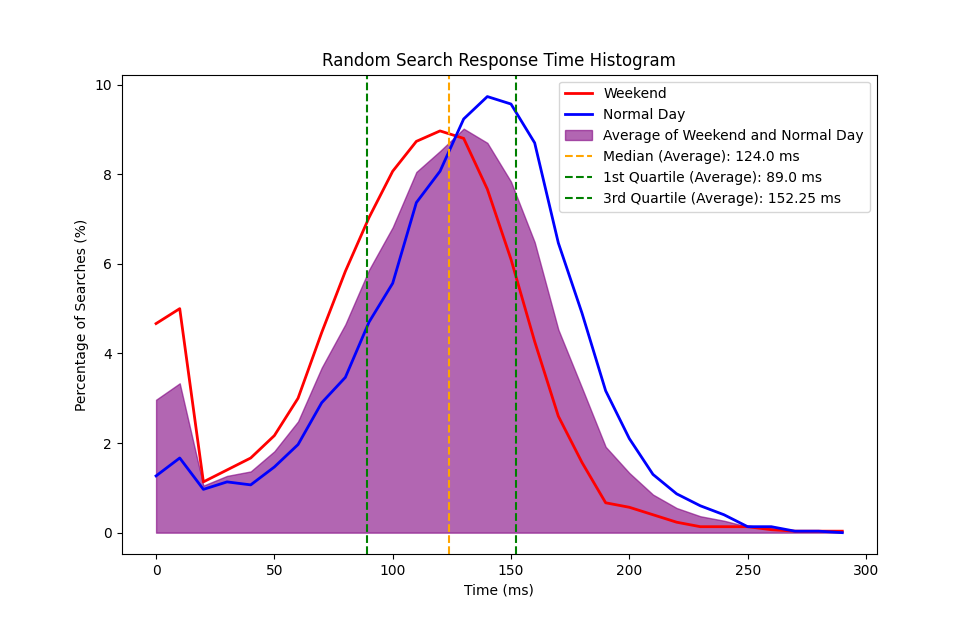
\includegraphics[width=\textwidth]{img/histogram.png}
    \caption{Histogram of response times}
    \label{fig:response_time_histogram}
\end{figure}

\begin{figure}[h!]
    \centering
    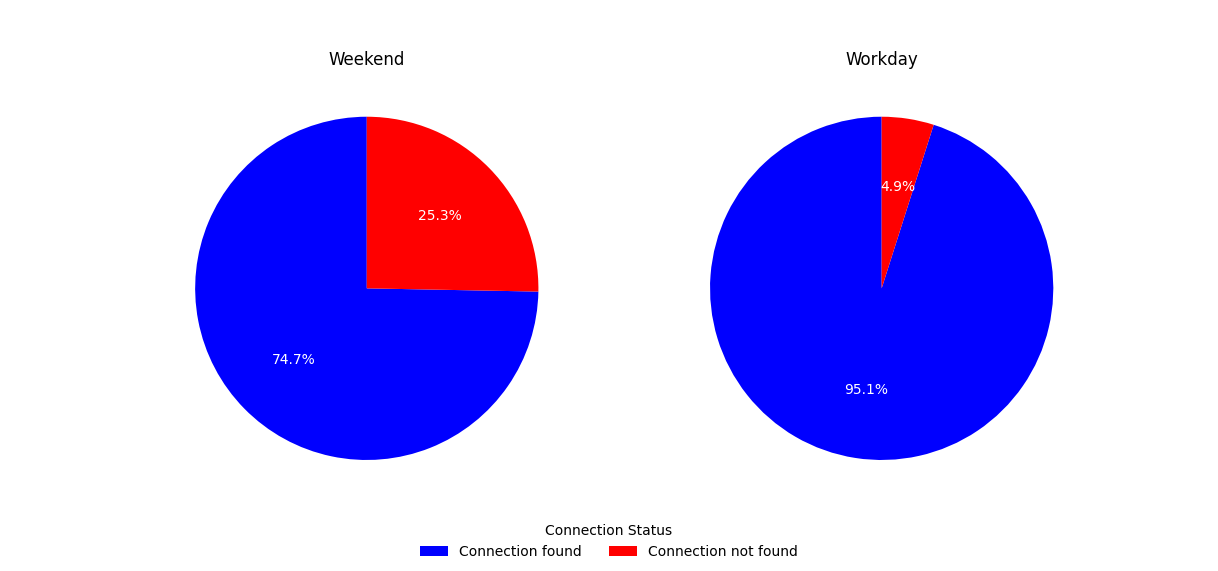
\includegraphics[width=\textwidth]{img/success_rates.png}
    \caption{Found connections rates}
    \label{fig:success_rates}
\end{figure}


\section{Client tests}

\subsection{User testing}

To properly test our client application and ensure that all functional requirements we set out to fulfill are met, we have prepared a list of test cases to perform manual user testing of the client. These contain the steps that the tester should perform and the expected results that these steps should lead to. We have performed all of these tests to ensure our application is working correctly. All the test cases can be found in the client repository.

\subsection{Usability testing}

\xxx{Results of questionnaire for alpha users}

\chapter*{Conclusion}
\addcontentsline{toc}{chapter}{Conclusion}

During the work on this thesis, we first analyzed the connection search problem and its existing solutions. We then used this information to set the requirements for our new app. To reach our goal of creating a more personalizable app, we added new requirements to solve some of the shortcomings of other existing app. We then analyzed what data is available to help us build the application and how to use it.

After this, we designed our application. We analyzed the algorithms that could be used to solve the problem and chose the most appropriate one. We went over programming languages that could be used for the project and chose the most suitable one. We have also chosen what high-level our application was going to have.

We implemented the application, which consists of a server and a client part. We documented the source code in detail, both inside the code-base using documentation comments and in this document, describing the structure of the code. We went over different decisions faced during the implementation and the solutions chosen. We also summarized information on the usage of external third-party software within our code. Lastly, we also explained in detail how to use the application, including documenting the installation process and usage of both the client and server apps. We also documented the usage of the server-side API.

Finally, we have tested our application in multiple ways. This includes automatized unit tests testing different components of the server application, tests checking the integrity of results returned by the server-side application, performance tests to find out the response times of the server application and usability tests to check that the client application provides the functionality it should.

We have achieved our goal of creating an application that offers more personalization and customization options than the existing solutions. We have also successfully incorporated bikesharing into our searches, being only the second application in Prague to do so. There are, however, still many opportunities for future expansion. These include implementing the client app for the iOS operating system as well, implementing useful features that other apps have, such as displaying the resulting connections on a map, displaying the exact stops every trip takes or providing information on the cost of tickets necessary to perform the connections. Thus, we might take this work and expand it in the future to provide a more robust, all-round solution than the scope of this work allowed us to.


%%% Bibliography
%%% Bibliography (literature used as a source)
%%%
%%% We employ biblatex to construct the bibliography. It processes
%%% citations in the text (e.g., the \cite{...} macro) and looks up
%%% relevant entries in the bibliography.bib file.
%%%
%%% See also biblatex settings in thesis.tex.

%%% Generate the bibliography. Beware that if you cited no works,
%%% the empty list will be omitted completely.

% We let bibliography items stick out of the right margin a little
\def\bibfont{\hfuzz=2pt}

\printbibliography[heading=bibintoc]

%%% If case you prefer to write the bibliography manually (without biblatex),
%%% you can use the following. Please follow the ISO 690 standard and
%%% citation conventions of your field of research.

% \begin{thebibliography}{99}
%
% \bibitem{lamport94}
%   {\sc Lamport,} Leslie.
%   \emph{\LaTeX: A Document Preparation System}.
%   2nd edition.
%   Massachusetts: Addison Wesley, 1994.
%   ISBN 0-201-52983-1.
%
% \end{thebibliography}


%%% Figures used in the thesis (consider if this is needed)
\listoffigures

%%% Tables used in the thesis (consider if this is needed)
%%% In mathematical theses, it could be better to move the list of tables to the beginning of the thesis.
\listoftables

%%% Abbreviations used in the thesis, if any, including their explanation
%%% In mathematical theses, it could be better to move the list of abbreviations to the beginning of the thesis.
\chapwithtoc{List of Abbreviations}

%%% Doctoral theses must contain a list of author's publications
\ifx\ThesisType\TypePhD
\chapwithtoc{List of Publications}
\fi

%%% Attachments to the thesis, if any. Each attachment must be referred to
%%% at least once from the text of the thesis. Attachments are numbered.
%%%
%%% The printed version should preferably contain attachments, which can be
%%% read (additional tables and charts, supplementary text, examples of
%%% program output, etc.). The electronic version is more suited for attachments
%%% which will likely be used in an electronic form rather than read (program
%%% source code, data files, interactive charts, etc.). Electronic attachments
%%% should be uploaded to SIS. Allowed file formats are specified in provision
%%% of the rector no. 72/2017. Exceptions can be approved by faculty's coordinator.

% \appendix
% \chapter{Attachments}

% \section{First Attachment}

\end{document}
